\documentclass[a4paper,12pt]{article}
\usepackage{amsmath,amsfonts,amsthm,amscd,amssymb,latexsym,eufrak}
%%%%%%%%%%%%%
\usepackage{caption}
\usepackage{subcaption}
\usepackage{enumerate,graphicx,psfrag}%,subfigure}%,jchangebar,oldgerm}
\usepackage[mathscr]{eucal}
\usepackage[usenames]{color}
\usepackage{url}
\usepackage[shortlabels]{enumitem}
\usepackage{comment}
\usepackage{showkeys}
%%%%%%%%%
\sloppy

%%\documentclass[12]{article}


%%%%%%%%%%%%%%%%%%%%%%%
%
%
%
\title{The subgroup membership problem
}
\author{Andrew J. Duncan, Elizaveta Frenkel}

\renewcommand{\a}{\alpha }
\renewcommand{\b}{\beta }
\newcommand{\G}{\Gamma }
\newcommand{\g}{\gamma }
\newcommand{\D}{\Delta }
\renewcommand{\d}{\delta }
%\def\vd{\vardelta}
\newcommand{\ep}{\epsilon }
\newcommand{\e}{\varepsilon }
\newcommand{\z}{\zeta }
%\eta
\renewcommand{\th}{\theta }
\newcommand{\T}{\Theta }
\renewcommand{\i}{\iota }
\renewcommand{\k}{\kappa }
\renewcommand{\l}{\lambda }
\renewcommand{\L}{\Lambda }
%\mu
%\nu
%\xi
%omicron
%\pi
\renewcommand{\r}{\rho }
\newcommand{\s}{\sigma }
\renewcommand{\S}{\Sigma }
\renewcommand{\t}{\tau }
\newcommand{\up}{\upsilon }
\newcommand{\U}{\Upsilon }
%\phi
\newcommand{\x}{\chi }
%\psi
\newcommand{\W}{\Omega }
\newcommand{\w}{\omega }
%%%%%%%%%%%%%%%%%%%%%%%%%%%%%%%
%%%%%%%%%%%%%%%%%%%%%%%%%%%%%
\newcommand{\pd}{\partial}
\newcommand{\wht}{\widehat}
%\newcommand{\cC}{{\mathcal C}}
%\newcommand{\cdim}{\texttt{cdim}}
\newcommand{\fC}{{\textswab C}}
\newenvironment{ef}{\noindent\color{blue} \bf EF: }{}
%
\newcommand{\cA}{{\cal{A}}}
\newcommand{\cD}{{\cal{D}}}
\newcommand{\cF}{{\cal{F}}}
\newcommand{\cH}{{\cal{H}}}
\newcommand{\cJ}{{\cal{J}}}

\newcommand{\cK}{{\cal{K}}}
\newcommand{\cP}{{\cal{P}}}
\newcommand{\cR}{{\cal{R}}}
\newcommand{\cS}{{\cal{S}}}
\newcommand{\cW}{{\cal{W}}}
\newcommand{\cQ}{{\cal{Q}}}
%\newcommand{\GG}{\ensuremath{\mathbb{G}}}
\newcommand{\pp}{\mathbf{p}}
%%%%%%%%%%%%%%%%%%%%%%%%%%%%%%
\newcommand{\nul}{\emptyset }

%%%%%%%%%%%%%%%%%%%%%%%%%%%%%%
\newtheorem{theorem}{Theorem}[section]
\newtheorem{lemma}[theorem]{Lemma}
\newtheorem{corollary}[theorem]{Corollary}
\newtheorem{proposition}[theorem]{Proposition}
\newtheorem{axiom}[theorem]{Axiom}
\newtheorem{definition}[theorem]{Definition}
\newtheorem*{defn*}{Definition}
\newtheorem{conjecture}[theorem]{Conjecture}
%cvs -d :pserver:najd2@cvs.mas.ncl.ac.uk:/CVS/najd2
\newtheorem{exam}[theorem]{Example}
%\newtheorem{comment}[theorem]{Comment}
%
%
\newenvironment{example}{\begin{exam} \rm}{\end{exam}}
%
%
%
\newtheorem{remk}[theorem]{Remark}
\newenvironment{remark}{\begin{remk} \rm}{\end{remk}}
%
%%%%%%%%%%%%
\numberwithin{equation}{section}
\numberwithin{figure}{section}
%%%%%%%%%%%%%%%%%%%%
\newcommand{\Iso}{\operatorname{Isom}}
\newcommand{\Aut}{\operatorname{Aut}}
%%%%%%%%%%%%%%%%%%%
\renewcommand{\AA}{\ensuremath{\mathbb{A}}}
\newcommand{\ZZ}{\ensuremath{\mathbb{Z}}}
\newcommand{\QQ}{\ensuremath{\mathbb{Q}}}
\newcommand{\RR}{\ensuremath{\mathbb{R}}}
\newcommand{\NN}{\ensuremath{\mathbb{N}}}
\newcommand{\CC}{\ensuremath{\mathbb{C}}}
\newcommand{\FF}{\ensuremath{\mathbb{F}}}
%\renewcommand{\ker}{\verb"Ker"}
\newcommand{\cC}{\mathcal{C}}
\renewcommand{\cF}{\mathcal{F}}
\newcommand{\cO}{\mathcal{O}}
\renewcommand{\cS}{\mathcal{S}}
\newcommand{\la}{\langle}
\newcommand{\ra}{\rangle}
%\newcommand{\BA}{\ensuremath{\mathbb{A}}}
%%%%%%%%%%%%%%%%%%%%%%%%%%%%%%%%%%%%%%
\newcommand{\maps}{\rightarrow}
\newcommand{\ov}[1]{\overline{#1}}
\newcommand{\bs}{\backslash}
%%%%%%%%%%%%%%%%%%%%%%%%%%%%%%%
\newcommand{\be}{\begin{enumerate}}
\newcommand{\ee}{\end{enumerate}}
\newcommand{\bd}{\begin{description}}
\newcommand{\ed}{\end{description}}
%%%%%%%%%%%%%%%%%%%%%%%%%%%%%%%%%%%
%
\newenvironment{ajd}{\noindent\color{red} AJD }{}
\newenvironment{xxx}{\noindent\color{red}}{}
%
\begin{document}
\maketitle

\begin{abstract}
Stallings folding theory is modified, using double coset representatives, and to applied 
to the study of subgroups of  amalgamated
products of finite rank free groups. As an application the 
 subgroup membership
problem for such groups is shown to be decidable. An algorithm for this
problem is constructed and its complexity is analysed.
 \end{abstract}



\section{Introduction}\label{se:global_intro}

Stallings introduced his technique of subgroup foldings in 
\cite{stallings83} where he applied it to investigate subgroups of 
free groups. In \cite{stallings88} Stallings extended ideas of
foldings to non-free actions of groups on graphs and trees. In the following 
years these ideas were widely generalised, in several
directions,  and used to solve a variety of  problems in
combinatorial group theory: see for example
\cite{befe,BoWei,KM02,SilvaWeil08}. 
In this paper we consider  subgroups
of free products with amalgamation of free groups of finite rank, using
a language of normal forms based on double coset representatives.  We
extend the theory  of Stallings foldings to this setting and use it to construct an
explicit algorithm for the subgroup membership problem.

Let $G = <X|R>$ be a finitely generated group. 
A fixed subgroup $K$ of $G$ is said to have 
\emph{solvable  membership problem} if there is an algorithm which, for
any word $w$ in $\FF(X)$, decides
whether or not $w$ represents an element of  the subgroup $K$. 
The group $G$ has 
\emph{solvable  (uniform) membership problem} if there is an algorithm which, for
any finite set of words $w, k_1, \ldots k_s$ in $\FF(X)$, decides
whether or not $w$ represents an element of  the subgroup $K = <k_1,
\ldots, k_s>$ of $G$. 

``Free group constructions'', in particular, free products of groups,
with or without amalgamation, $HNN$-extensions
 and, more generally, fundamental groups
of graphs of groups constitute a subject of special significance in
group theory, from many points of view. Initial results in this area, 
related to the solvability of membership problem,  due to Mihailova (see
\cite{mi59,mi68}), show that the membership problem is
decidable in the free product of groups $A$ and $B$ if it is decidable
in both factors. Another famous result of
Mihailova \cite{mi58}  provides an important counter-example:
 namely,  a finitely generated
subgroup of a direct product of two free groups of rank two with
unsolvable membership problem.  This direct
product can in fact be considered as a sequence of two $HNN$-extensions
of rank two free group. On the other hand, another classical
result \cite[Proposition 2.21]{LS} shows that a free group of finite rank has solvable (uniform)
membership problem. Thus,  even innocent group
constructions can dramatically affect solvability of the membership problem.

The membership problem for free products with amalgamation and
$HNN$-extensions was studied by Bezverkhnii in papers
\cite{bez81,bez86,bez90,bez91}, using  combinatorial
techniques and standard normal forms for  amalgamated products of
groups. Our approach is, first of all, more geometric, and since
we have an eye on the generalisation of results to other free
constructions, we were obliged to introduce another language to
study these constructions. 
{\ajd What is the other language?} 
Another significant step in development of the theory of foldings for  free constructions 
 was taken by Kapovich, Miasnikov and Weidmann 
\cite{KMW03}, where the authors investigated the uniform membership
problem for fundamental groups of graphs of groups, under certain
assumptions on both vertex and edge groups. In particular, they
showed that, in the case where all vertex groups are either locally
quasiconvex word hyperbolic or polycyclic-by-finite, and all edge 
groups are polycyclic-by-finite; the uniform membership problem for the 
fundamental group of the graph of groups is solvable.

As mentioned above, we  introduce a  geometric
technique, which relies on Stallings foldings and 
normal forms based on double cosets, for elements of amalgamated products of
groups. 

Now, a few words on the structure of the paper. In Section
\ref{sec:dcforms} we introduce double coset repreesentatives for
elements of free groups, with respect to a fixed subgroup,  
%These representatives are used to define double coset normal forms 
%We show that these representatives 
%are unique 
and  
  describe an explicit procedure
 for their construction. 
These representatives are used to define unique double coset normal forms 
for elements of 
amalgamated products of finite rank free groups in Section  \ref{sec:foldings}, which
 is the heart of the paper. For a subgroup $K$ of such an amalgam, we 
describe a generalised folding process, which begins with the flower automaton
of $K$, over an extended alphabet, and results in  
a ``double coset graph'' for $K$, which  recognises 
precisely the  normal forms of elements of $K$.

In Section \ref{sec:TC} we estimate the time complexity of
algorithms described in the previous parts of the paper. In
particular, we illustrate how quickly the  preparatory
work in construction of  double coset normal forms of generators
for $K$  can be carried out; we calculate  the complexity of the process of modification of
components of the flower automaton of $K$, and of the reassembly process required to 
produce the double coset graph.

The authors are grateful to Vladimir Remeslennikov for suggesting the use of double cosets and 
for helpful
discussions,  and to Christian Perfect who gave invaluable help with programming.


\begin{comment}
\section{Double coset normal form}\label{sec:intro}
Based on notes copied (laboriously) from Christian's page
\url{
http://checkmyworking.com/misc/writemaths/?doublecoset
}

$F_1$, $F_2$ free groups (finitely generated by $X_1$
and $X_2$, respectively).

Let $H_1 \leq F_1$, $H_2 \leq F_2$ such that
there exists an isomorphism $\phi: H_1 \rightarrow H_2$.

i.e. we have finite bases $\{h_1, \ldots, h_m \}$  for $H_1$ and
$\{h_1', \ldots, h_m'\}$ for $H_2$.

Consider the free group $\FF(Z)$, generated by $Z=\{z_1, \ldots, z_m\}$,
and the maps $\phi_1$ and $\phi_2$ such that
$\phi_1(z_i)=h_i(X_1)  $ and  $\phi_2(z_i)=h^\prime_i(X_2)$, $i=1,\ldots ,m$.
Thus $\phi_i$ extends to an isomorphism of $\FF(Z)$ to $H_i$. We choose
the $\phi_i$ so that $\phi=\phi_2\phi_1^{-1}$.

Let ${G = F_1 \underset{H_1=H_2}{\ast} F_2}$, the group with
 presentation \[\la X_1,X_2 | h_i = h_i', i=1, \ldots ,m\ra.\]

A  set $S_i \subseteq F_i$ such that
\be
\item
$F_i = \displaystyle{\bigcup_{s \in S_i} H_isH_i}$
and
\item
for all $s, s^\prime \in S_i$, $s\in H_i s^\prime H_i$
implies $s=s^\prime$,
\ee
is called a set of \emph{double coset representatives for} $H_i\le F_i$.

Let $S_1$ and $S_2$ be sets of  double coset representatives of
$H_1\le F_1$ and $H_2\le F_2$, respectively. Let $g \in G$.
A word $w$ representing $g$ is in \emph{(double coset) normal form} if
$w = h_{0}p_1h_{1}p_2 \cdots h_{k-1}p_kh_{{k}}$, $k\ge 0$,  with
\be
\item $p_i \in S_1\cup S_2$  and $h_i$ is a reduced word in $\FF(Z)$ and
\item if $p_i\in S_j$ then $p_{i+1}\notin S_j$, for $j=1$ and $2$,
\ee
for $i = 1, \ldots ,k$.
\end{comment}

\section{Constructing double coset representatives}\label{sec:dcforms}
\subsection{Free products with amalgamation}\label{sec:intro}

We denote the free group on as set $X$ by $\FF(X)$. 
 By a {\em reduced} word in $\FF(X)$  we mean
 a freely reduced word in $(X\cup X^{-1})^\ast$, and we write $w\in \FF(X)$
to mean that $w$ is a reduced word. For $u,v, w\in \FF(X)$ we
write $w=u\circ v$ if $|w|=|u|+|v|$, in which case we say that $u$ is a {\em prefix}
of $w$.

Let $X_1$ and $X_2$ be disjoint,
finite sets and let 
$F_1=\FF(X_1)$ and $F_2=\FF(X_2)$.
Let $H_1 \leq F_1$ and  $H_2 \leq F_2$ be finitely generated subgroups of rank $m$,
freely generated by $\{h_1,\ldots, h_m\}$ and  $\{h_1', \ldots, h_m'\}$, respectively. 
Denote by $\phi$ the isomorphism of $H_1$ to $H_2$ which maps $h_i$ to  $h_i^\prime$, 
for all $i$. 
%Then, if $Z=\{z_1, \ldots, z_m\}$ is a set (disjoint from $X_1\cup X_2$), the maps 
% $\phi_1$ and $\phi_2$, such that
%$\phi_1(z_i)=h_i\in F_1$ and  $\phi_2(z_i)=h^\prime_i\in F_2$, $i=1,\ldots ,m$, 
%determine isomoprhisms from $\FF(Z)$ to $H_1$ and $H_2$. 
 Now let $G = F_1 \underset{H_1=H_2}{\ast} F_2$ be the free product  of $F_1$ and $F_2$, amalgamating $H_1$ and $H_2$: that is $G$ is the group 
 with
 presentation \[\la X_1\cup X_2 | h_i = h_i', i=1, \ldots ,m\ra.\]

%%%%%%%%%%
Given an arbitrary word $g\in F_1\ast F_2$,
we should like an algorithm to write $g$ in 
some normal form with uniqueness. As a first attempt, 
 we say $g$ is in \emph{reduced form} if either $g$ is the empty word $1$, or $g = g_1 \cdots g_t$, where
\begin{itemize}
\item 
$g_1 \in F_1$ or $g_1 \in F_2$ and, if $t=1$ then $g_1\neq 1$,  and 
\item 
for
$i > 1$,    $g_i \in (F_1 \backslash H_1)\cup (F_2\backslash H_2)$ and
\item for $i\ge 1$,   $g_i$
and  ${g_{i+1}}$ belong to  different factors. 
\end{itemize}
As the membership problem
is solvable in $F_1$ and $F_2$ we may write elements in reduced form: for example, 
to write $g$ in reduced form,
we can use the following procedure. 
First write $g$  as a reduced word in $F_1\ast F_2$, so $g=f_1\cdots f_t$, where
each $f_i$ belongs to a factor and 
consecutive $f_i$ come from different factors, $F_1$ or $F_2$. Then apply the
following process. 
\be[Step 1]
\item\label{it:st1} For $i=1,\ldots ,t$ do the following.
Write each $f_i$ as  a reduced word in $F_1$ or $F_2$ as appropriate.  
If $f_i\in F_k$ then,  
using an algorithm for the membership problem in $H_k$, check whether or not $f_i \in H_k$.
 If none of the $f_i$'s lies in $H_1$ or $H_2$ then
$g= f_1 \cdots f_t$ is in  reduced form.  
\item  Now suppose that some $f_i \in H_k$,  and let  $i$ be the
minimal index with this property. Then $\phi^{\pm 1}(f_i)=c\in H_{l}$, $l\neq k$.  
If $i = 1$, rewrite $g$  in the
form $g = f'_2 f_3 \cdots f_t$,  where  $f'_2 = cf_2$, an element of $F_1\cup F_2$.  
If $i > 1$ then rewrite $g$ as
$g = f_1 \cdots f_{i-2} f'_{i+1}f_{i+2} \cdots f_t$, where
$f'_{i+1} = f_{i-1}c f_{i+1}\in F_1\cup F_2$. Return to 
\ref{it:st1}.
\ee

The reduced form is easy to calculate and gives a solution to the word problem: since
a reduced form with $t>0$ cannot represent the identity \cite[Theorem 2.6]{LS}. 
However reduced forms do not uniquely represent  
 elements of $G$. To resolve this non-uniqueness problem it is common to 
chose a set of coset representatives of $H_k$ in $F_k$, $k=1,2$, and use these to rewrite
the reduced form. If $T_k$ is a set of right coset representatives of $H_k$ then 
 a word $g\in F_1\ast F_2$ is in \emph{single coset normal form} (or \emph{sc-normal form}) if 
\[g=ct_1\cdots t_r,\]
where $c\in H_1$, $t_i\in T_1\cup T_2$, $t_1\neq 1$, and consecutive $t_i$ are from 
different factors. Every element of $G$ can be \emph{uniquely} expressed as a word in single coset
normal form \cite[Theorem 4.4]{MKS}. 
Coset representatives can be found using Stallings automata, which we describe below, so
there is a procedure for writing elements in sc-normal form. Namely: 
having written an element $g$ in reduced form, 
working from right to left, for each $i$  
 we express $f_i$ in the 
form $c_it_i$, where $c_i\in H_k$ and $t_i\in T_k$. The element $f_{i-1}$ must then be replaced
by $f_{i-1}\phi^{\pm 1}(c_i)$, before being rewritten. Continue this way till the
left hand side of the word is reached. 

In this process the coset representative of 
$f_{i-1}$ with respect to $H_l$ will not, in general, be known 
 until $f_i$, ..., $f_t$ have been rewritten, and moreover each step requires an application
of the map $\phi$ or its inverse. As we shall see, when we write words in terms of 
double
coset normal forms the algorithm is simpler, and the coset representatives that
occur in any reduced  form of a word are the same as 
the double coset representatives of the final double coset normal form.

To write elements in terms of single or double coset representatives we use Stallings automata, 
which we now define. In the following subsection we shall then define double coset representatives. 
\begin{comment}
with respect to some choice of double coset representatives. We may
assume (after free cancellation if necessary) that $g$ is a
reduced word in $((X_1\cup X_2)\cup ( X_1^{-1}\cup X_2^{-1}))^\ast$.

First we say $g$ is in \emph{reduced form} if $g = g_1 \cdots g_t$, where
$g_1 \in F_1$ or $g_1 \in F_2$ and
for
$i > 1$,    $g_i \in (F_1 \backslash H_1)\cup (F_2\backslash H_2)$ and  $g_i$
and  ${g_{i+1}}$ belong to  different factors. As $F_1$ and
$F_2$ have solvable membership problem we can write $g$ in
reduced form. More precisely, we construct a Stallings automaton
(see below) $A_k$ for
$H_k\le F_k$, $k=1,2$. % and choose a maximal subtree $T_k$ of $A_k$.
Then we write $g=f_1\cdots f_r$, in free product normal form (each
$f_i$ is in a factor and successive terms are from different
factors). Now, using the appropriate Stallings automaton $A_k$, we
write $f_r=h_rg_r$, where $h_r$ is the maximal prefix of $f_r$
accepted by $A_k$ and $g_r$ is
 the
unique word such that $f_r=h_rg_r$, reduced as written.

Using the maps $\phi_1$ and $\phi_2$ we now write $h_r$ in terms
of the generators of the other factor, to obtain $h^\prime_r$ and
then replace $f_{r-1}$ with $f_{r-1}^\prime=f_{r-1}h^\prime_r$.
Now start again with $f_{r-1}^\prime$ instead of $f_r$. Continue
till the word is exhausted. This gives $g=g_1\cdots g_t$ in
reduced form. {\ef To rewrite a non-reduced word to its reduced
form, one can use a simpler algorithm. You are rewriting elements
in the canonical normal form (and it depends on a choice of $T_k$
as well). To represent element in a (non-unique) reduced form, we
care only about factors $f_i$ which belong to a subgroup $H_k$.
For instance, we can use the following algorithm.


To rewrite in double coset normal form we need to
 rewrite
each $g_i$ in double coset normal form in its factor, with respect
to some (fixed) set of double coset representatives. We show how
this can be done below.
\end{comment}
\subsection{Automata and Stallings Foldings}\label{sub:foldings}

An {\em automaton} $A$ is  a quintuple
$(\S,Q,\d,\mathcal{S},\mathcal{F})$, where $\S$ is finite set
called the {\em alphabet}, $Q$ is a finite set of {\em states},
$\d$ is a map $\d:Q\times \S\maps Q$, called the {\em transition
function}, $\mathcal{S}\subset Q$ is the (non-empty) set of {\em
start states} and $\mathcal{F}\subseteq Q$ is the set of {\em
final states}.  If
$\mathcal{F}=\{s_0\}=\mathcal{S}$ it's common to drop
$\mathcal{F}$ from the description and define $A$ as a quadruple.
For details of the theory of automata the reader is referred to
 \cite{Lawson04}.

By a graph we mean a finite, directed, edge labelled graph.
We shall associate to an automaton $A$
a graph $\G_A$ with vertices
$V=V(\G_A)=Q$; edge set $E=E(\G_A)$ consisting of elements
$(u,\s,v)$ of $Q\times \S\times Q$ such that $\d(u,\s)=v$; and
labelling function $l:E\maps \S$ given by $l(u,\s,v)=\s$, for all
$(u,\s,v) \in E$.  If $\mathcal{S}$ and $\mathcal{F}$ are the sets
of start and final states of $A$ we sometimes write
$(\G_A,\mathcal{S},\mathcal{F})$ for
$(\S,Q,\d,\mathcal{S},\mathcal{F})$, and in addition if
$\mathcal{S}=\{s_0\}$ and $\mathcal{F}=\{f_0\}$, we may abbreviate
this to $(\G_A,s_0,f_0)$. If $\mathcal{S}=\{s_0\}=\mathcal{F}$
we
call $s_0$ the {\em root}
vertex of $\G_A$ and say that $A$ and $\G_A$ are {\em rooted}. We may
 write $(\G_A,s_0)$ for $(\G_A,s_0,f_0)$ if this is the case.  For notational simplicity we identify $\G_A$
and $A$ whenever it is convenient and does no ambiguity arises.

By a path $p$
in a graph we mean a sequence $(v_0,e_1,v_1, \ldots , e_n ,v_n)$ of
 vertices $v_i$ and edges $e_i$ such that
 $e_i=(v_{i-1},\s_i,v_i)$, for $i=1,\ldots ,n$.
The
label $l(p)$ of this  path is defined to be
 the concatenation $\s_1\cdots \s_n$ of the labels of the
edge sequence of $p$.  If $w$ is the label of a path
in $\G_A$, from a vertex of $\cS$ to a vertex of $\cF$, then we
say that $w$ is accepted by $A=(\G_A,\cS,\cF)$. The set of all
words in the free monoid $\S^*$, generated by $\S$, which are
accepted by $A$  is called
the {\em language accepted by} $A$ and denoted $L=L(A)$.
We extend this terminology, for an automaton
$A=(\S,Q,\d,\mathcal{S},\mathcal{F})$,
to say that a  word $w$ is {\em readable}
by $A$ if $w$ is in the
language accepted by $(\G_A,\cS,Q)$  and define
\[L_Q=L_Q(A)=\{w:w \textrm{ is readable by } A\}.\]
If $\S$ is a
subset of a group $G$ (and whenever $a,a^{-1}\in \S$ then $a^{-1}$ is
the inverse of $a$)
 then the  natural map from $L_Q(A)$ to
$G$ is denoted $\pi:L_Q(A)\maps G$.

%%{\ef In chapter 4  we use these terms (readable and accepted) not
%%only for initial and final states, but for arbitrary states
%%(boundary vertices etc.). Is it better to extend the definitions
%%here?}
%%{\ajd I tried to set things up so the definitions cover what we
%%do in Section 4. To change the start and final states from $s$ and $f$
%%to $\a$ and $\b$,  change the
%%automaton from $(\S,Q,\d,s,f)$ to $(\S,Q,\d,\a,\b)$. I may not have
%%actually written this in the appropriate places.}
%% Ok, it is written and I've checked, everything agree with given definitions.


An {\em involutive alphabet} is a set $\S$ of the form $\{a_1, \ldots, ,
a_r, a_1^{-1}, \ldots, a_r^{-1}\}$.
The automaton $A =(\S, Q, \d,\mathcal{S},\mathcal{F})
= (\G_A, \mathcal{S}, \mathcal{F})$ is {\em
involutive} if $\S$ is an
involutive alphabet and, for all $p, q \in Q$ and $a \in \S$,
$\d(p,a)=q$ if and only if $\d(q, a^{-1})=p$ (that is $(u, a, v) \in E
\Leftrightarrow (v, a^{-1}, u) \in E$).
In diagrams of involutive automata an edge labelled $a$  from
$u$ to $v$  represents
both $(u,a,v)$ and $(u,a^{-1},v)$.  

From now on we will
consider only involutive automata and, moreover, we always assume that $\S$ is a subset of a group.
The automaton $A$
is {\em deterministic}  or {\em folded} if $\d(p,a)=q$ and
$\d(p,a)=q'$ imply $q=q'$ (that is, $(u, a, v)
\in E$ and $(u, a, v^\prime) \in E$ imply $v=v^\prime$).
We say an automaton $A$ is \emph{connected} if $\G_A$ is connected.
(For an involutive rooted automataton being connected is equivalent to the property that 
for every vertex $q$ there is a path from $q$ to the root and a path from the root to $q$. 
Automata with this property are usually called \emph{trim}, but since the two properties are 
equivalent in our setting we use the more intuitive nomenclature.)
Finally, an involutive, rooted, connected, deterministic,
automaton, with a single final state, is called an {\em inverse}
automaton.

Let $A=(\G_A,s_0,f_0)$ be an inverse automaton.
If $w$ is readable by $A$ then there exists a
unique vertex  $\t(w)$ of $\G_A$ such that $w$ is accepted by
$(\G_A,s_0,\t(w))$: we call $\t(w)$ the {\em terminal vertex} of $w$. ($L$ is the set of words $w$ readable by $A$ with
$\t(w)=s_0$.)
Fix a spanning tree $T$ for $\G_A$. For each vertex $v$ of $\G_A$
let $w(v)$ denote the label of the path in
$T$ from $s_0$ to $v$.  Define
\[L_T=L_T(A)=\{w(v): v \textrm{ is a vertex of } A\}.\]
Thus $L\subseteq L_T\subseteq L_Q$. 

If $w, s, u\in \FF(X)$ with $w=s\circ u$ then we say that $s$ is
\be[(i)]
\item
 an $L_Q${\em -prefix} of $w$ if $s\in L_Q$;
\item
an % {\em maximal}
$L_T${\em -prefix} of $w$ if $s\in L_T$.
\ee
An $L_Q$ or $L_T$-prefix $s$ of $w$ is  {\em maximal} if no longer
subword of $w$ is an $L_Q$ or $L_T$-prefix, respectively.

Since we identify the automaton $A$ with the graph $\G_A$, we
ascribe properties of automata (like rooted, connected,
involutive, folded or inverse) to graphs in general and $\G_A$ in
particular.

%%Let $A=(V,E,s_0)$ and $A^\prime=(V^\prime,E^\prime,s^\prime_0)$ be
%%two automata. A {\em morphism} $A \rightarrow A^\prime$ is a map
%%$\varphi: V \rightarrow V^\prime$ such that $\varphi(s_0) =
%%s^\prime_0$ and $(p,a,q) \in E \Rightarrow
%%(\varphi(p),a,\varphi(q)) \in E^\prime$.
We now recall the notion of a Stallings folding of an automaton,
which we will use directly, to construct Stallings automata for
subgroups of free groups, and in generalised form to produce
dc-resolutions of automata (in Section \ref{sec:foldings}). For
more details on Stallings foldings  and  Stallings automata  see
\cite{ventura11} or \cite{BartholdiSilva}.

An {\em elementary folding} of a rooted, directed, labelled
graph $(\G,s_0)$ is a
graph $(\G^\prime,s^\prime_0)$ obtained from $(\G,s_0)$ as
follows. Suppose that $e=(u, \s, v)$ and $e^\prime=(u, \s,
v^\prime)$ are edges of $\G$. (We do not require $u$, $v$ and
$v^\prime$ to be distinct.)
 Then $\G^\prime$ is the quotient of $\G$ formed by identifying
$v$ and $v^\prime$, to form a new vertex $v^{\prime\prime}$; and
$e$ and $e^\prime$, to form a new edge $e^{\prime\prime}=(u, \s,
v^{\prime\prime})$. If $s_0= v$ or $s_0 = v^\prime$ then
$v^{\prime\prime}$ is the root of $\G^\prime$ and otherwise
$s^\prime_0=s_0$.
 A {\em folding} of a graph $\G$ is a graph obtained
from $\G$ by a finite sequence of elementary foldings.

If a rooted graph $\G$ is not folded then a folding may be applied; reducing the
number of edges of the graph. Continuing this way a folded graph may eventually
be produced. It follows that  folded (i.e. deterministic) graphs are precisely those
to which no elementary folding may be applied.

A morphism of automata $\G_A$ and $\G_{A^\prime}$ is a map
$\theta: \G_A\maps \G_{A^\prime}$ which maps vertices to vertices and
edges to edges in such a way that 
\be \item if $s$ is a start state  of
$\G_A$ then $\theta(s)$ is a start state of $\G^\prime$; 
\item if $t$ is a final state of $\G$ then $\theta(t)$ is a final state of
$\G^\prime$ and
\item  if
$(u,\sigma,v)$ is an edge of $\G$ then
$\theta(u,\sigma,v)=(\theta(u),\sigma,\theta(v))$. \ee An
elementary folding of  $(\G,s_0,t)$ to $(\G^\prime,s^\prime_0,
t^\prime)$ induces a morphism from $\G$ to $\G^\prime$: namely the
quotient map. Therefore there is
 a uniquely determined {\em folding morphism}  from $\G$ to any folding. Moreover, if $\G_1$
is a folding of $\G$ and $\theta$ is the folding morphism then
$\pi(L(\G,s,t))= \pi(L(\G_1,\theta(s),\theta(t)))$.




Let $Y=\{w_1,\ldots ,w_n\}$ be a generating set for $H$, where $w_i\in F$.
The {\em flower automaton} $\G_Y(H)$, of $H$ (with respect to this generating set)
is the graph constructed as follows. For each $i$ let $C_i$ be a cycle
graph with $|w_i|$ vertices, and choose a vertex $v_i$ as the root. Direct
and label the edges of $C_i$, with elements of $X$,
so that the simple closed path based at $v_i$ has
label $w_i$ (read in, say, a counter-clockwise direction). The flower
automaton $G_Y(H)$ is formed by identifying all the vertices $v_i$ to form
a new graph, with root $v$ the image of the $v_i$. If $L_Y$ is the language  accepted
by $(\G_Y(H), v)$ then $\pi(L_Y)=H$.


The flower automaton of $H$ depends on the chosen generating set, and is,
in general,
non-deterministic (at the root vertex $s$). Stallings \cite{stallings83}
proved that the folded graph $\G(H)$, obtained by applying foldings to the
flower automaton of $H$ until the result is folded, is an inverse
automaton, independent of the generating set chosen.
Moreover  $(\G(H),s)$ is the minimal (fewest states) automaton accepting
every reduced word representing an element of $H$. (See \cite{BartholdiSilva}
for a proof in terms of automata.)
\begin{definition}
The automaton $(\G(H),s)$ is  called the {\em Stallings automaton} of $H$.
\end{definition}
\subsection{Double coset representatives in free groups}\label{sub:2cosetrepr}
Let $X$ be a finite alphabet, $F=\FF(X)$ and $H$ a finitely generated subgroup
of $F$.
A  set $S\subseteq F$ such that
\be
\item
$F = \displaystyle{\bigcup_{s \in S} HsH}$
and
\item
for all $s, s^\prime \in S$, $s\in H s^\prime H$
implies $s=s^\prime$,
\ee
is called a set of \emph{double coset representatives for} $H\le F$.

%%%%

Let $A$ be the Stallings automaton for $H$, and let  $s_0 =
1$ be its start state.
We shall define a set of double coset representatives for $H$ in two parts.
We begin with the definition of the first type of representative.
\begin{definition}[Double coset representative, type 1]
A word $w\in \FF(X)$ is a {\em (double coset) representative of
type} $1$ if
\[w=s\circ e \circ t^{-1},\]
where $e\neq 1$, $s$ is a maximal $L_Q$-prefix and an $L_T$-prefix of $w$,
and $t$ is a maximal $L_Q$-prefix and an
$L_T$-prefix of $t\circ e^{-1}$. Let $S^{(1)}$ denote the set of all representatives of type $1$.
\end{definition}


To describe the remaining representatives we shall first define an equivalence
relation on the ordered pairs of distinct vertices of $A$. Let
\[P=\{(u,v)\in V(A)\times V(A): u\neq v\}.\]
Define a relation $\sim$ on $P$ by $(u_0,u_1)\sim (v_0,v_1)$ if and only if
there exist paths $p_0$ and $p_1$ in $A$, from $u_0$ to $v_0$ and $u_1$ to $v_1$
respectively, such that $l(p_0)=l(p_1)$. (We allow these paths to have length $0$.)
Then $\sim$ is an equivalence relation on $P$.

\begin{lemma}\label{lem:equiv_verts}
Let $(u_0,u_1)$ and $(v_0,v_1)$ be elements of $P$ and let
$a_0=w(u_0)$, $a_1=w(u_1)$, $b_0=w(v_0)$ and $b_1=w(v_1)$. Then
$(u_0,u_1)\sim (v_0,v_1)$ if and only if there exist $h_0,h_1\in H$ such that
\[a_0a_1^{-1}=h_0b_0b_1^{-1}h_1^{-1}.\]
\end{lemma}
\begin{proof}
$\Rightarrow$: Let $p_0$ and $p_1$ be paths, from $u_0$ to $v_0$ and $u_1$ to $v_1$
respectively, such that $l(p_0)=l(p_1)=c$, say. Set $h_0=a_0cb_0^{-1}$ and
$h_1=a_1cb_1^{-1}$. Since $h_0$ and $h_1$ are labels of closed paths in $A$, based at $1$, we
have $h_0$ and $h_1$ in $H$. Thus
$a_0a_1^{-1}=h_0b_0c^{-1}cb_1^{-1}h_1^{-1}=h_0b_0b_1^{-1}h_1^{-1}$, as required.

$\Leftarrow$: Let $h_0$, $h_1 \in H$ such that $a_0a_1^{-1}=h_0b_0b_1^{-1}h_1^{-1}$.
Set $k=a_0^{-1}h_0b_0=a_1^{-1}h_1b_1$. Then $h_0=a_0kb_0^{-1}$ and $h_1=a_1kb_1^{-1}$
belong to $H$ so there exist paths $p_0$ and $p_1$ in $A$,
from $\t(a_0)=u_0$ to $\t(b_0)=v_0$ and
$\t(a_1)=u_1$ to $\t(b_1)=v_1$, both with labels $k$.
Therefore $(u_0,u_1)\sim (v_0,v_1)$.
\end{proof}

%%{\ef
%%It seems like we should specify different cases , depending on
%%$u_0, v_0$ and $u_1,v_1$ belonging to the same loop $h_i$ or not;
%%or something like this. Take an equivalence class as in example
%%\ref{ex:f_1f_2}. Then $a_0 = y_2^{-1}y_1$, $a_1 = y_1^2$, $b_0 =
%%y_2^{-1}$, $b_1=y_1$. Further, we obtain $c = y_1$ and the
%%equality satisfies, but with elements $h_0 = y_2^{-1} y_1^2 y_2$
%%and $h_1 = y_1^2$ which are not in $H_2$, as far as I understand.
%%Am I right or I misunderstood something?
%%}

To work with the equivalence relation $\sim$ its useful to define
the product of graphs. Given (labelled, directed)
graphs $\G_1$ and $\G_2$ we define the {\em
product} graph $\G_1\times \G_2$ to be the graph with vertices
$V=V(\G_1)\times V(\G_2)$ and with a directed edge labelled $a$
from $(u_1,u_2)$ to $(v_1,v_2)$ if and only if there are edges
$(u_1,a, v_1)$ and $(u_2,a,v_2)$ in $\G_1$ and $\G_2$,
respectively. If $\G$ is a graph then
vertices of $\G\times \G$ of
 the form $(v,v)$ are called {\em diagonal vertices}.
% We call the graph formed from  $\G\times \G$ by removing
% the diagonal vertices (and all incident edges) the
%{\em non-diagonal subgraph of} $\G\times \G$.
Note that if $\G$ is folded there is no edge of $\G\times \G$
joining a diagonal vertex to a non-diagonal vertex. In this case
it follows that the diagonal vertices are the vertices of a
connected component of $\G\times \G$, which is isomorphic to $\G$,
and that no other connected component contains a diagonal vertex.

In this notation $P$ is the set of non-diagonal vertices of
$\G_A\times \G_A$ and $(u,v)\sim (u',v')$ if and only if there is
a path from $(u,v)$ to $(u',v')$ in $\G_A\times \G_A$.
 Thus, as $\G_A$ is folded, the equivalence class of $(u,v)\in P$
is the set of vertices of the connected component of $\G_A\times \G_A$
containing $(u,v)$.

We shall choose one double coset representative corresponding to
each $\sim$ equivalence class. First observe that if
$(u,v)\in P$ and $w(u)=a\circ x$, $w(v)=b\circ x$, for some
$a,b\in \FF(X)$ and $x\in X^{\pm 1}$, then $(\t(a),\t(b))\in P$ and
$(u,v)\sim (\t(a),\t(b))$. It follows that every equivalence  class
of $\sim$ contains an element $(u',v')$ such that
$w(u')w(v')^{-1}$ is a reduced word; and representatives of each
equivalence class will be chosen to have this property.
%We make a choice $(u,v)$ of representative of each equivalence class
%of $\sim$ so that
%$w(u)w(v)^{-1}=w(u)\circ w(v)^{-1}$), in the next definition.

\begin{definition}\label{def:repres_t2}
Let $\pp$ be an equivalence class of $\sim$ and let $Y$ be the set
of all pairs $(u,v)\in \pp$ such that $|w(v)|$ is minimal (amongst
elements of $\pp$). Choose $(u,v)\in Y$ such that $|w(u)|$ is
minimal (amongst elements of $Y$) and define $(u,v)$ to be the
$\sim$ {\em representative} of
$\pp$. %Fix one $\sim$ representative for each equivalence class of$\sim$ and
Let $P_0$ denote the set of  all these $\sim$
representatives.

A word $w\in \FF(X)$ is
 a {\em (double coset) representative of type} $2$
if $w=w(u)w(v)^{-1}$, for some $(u,v)\in P_0$.
Let $S^{(2)}$ denote the set of all representatives of type $2$.

For each $(u,v)$ in $P$ choose a path in $\G_A\times \G_A$
from $(u,v)$ to the $\sim$ representative
$(u_0,v_0)$ of $(u,v)$ and define the {\em connecting element}
$c(u,v)$  of $(u,v)$ to be the label of this path.
\end{definition}
The  connecting elements enable systematic rewriting of certain
elements of $\FF$ in terms of representatives of type 2, as will be
seen below.
\begin{definition}
Define $S=S^{(1)}\cup S^{(2)}$.
\end{definition}


\begin{proposition}\label{prop:dcreps}
$S$ is a set of double coset representatives for $H$.
\end{proposition}
\begin{proof}
First we shall show that every element $w\in \FF(X)$ lies in $HdH$,
for some $d\in S$. In fact we describe an algorithm which
rewrites a given word $w$ in this form.

Assume that the Stallings automaton $A$ for $H$ has been constructed by folding from
given generators for $H$. A spanning tree $T$
for $A$ may then be chosen and the
set $L_T$ computed.
To find the equivalence class of a pair $(u,v)\in P$ the
graph $\G_A\times \G_A$ is constructed. As we pointed out above, $(u',v')\sim
(u,v)$ if and only if there is a path in $\G_A\times \G_A$ from $(u',v')$
to $(u,v)$. Therefore the $\sim$ equivalence class of $(u,v)$ is the
vertex set of the connected component of $\G_A\times \G_A$ containing
$(u,v)$.
Having constructed the equivalence classes of $\sim$
 a set of $\sim$ representatives may be constructed, by considering the
lengths of $w(a)$ and $w(b)$ for all $(a,b)$ in an equivalence class. Thus the
set $P_0$ and the connecting element $c(u,v)$, of each element
$(u,v)\in P$, may be computed at this stage.   \\

\noindent{\bf Algorithm I}.\\
Input $w\in \FF(X)$.
Let $h$ be the maximal prefix of $w$ accepted by $A$; so $h\in H$ and
$w=h\circ f$, for some $f\in \FF(X)$. Now use $A$ to find the maximal
$L_Q$-prefix $p$
of $f$ (i.e. the maximal prefix readable by $A$). Then
  $f= p\circ q$, for some $q\in \FF(X)$.

Next find the maximal prefix $g$ of $q^{-1}$ acceptable by $A$: say
$q^{-1}=g\circ r$, for some $r\in \FF(X)$, and then the maximal $L_Q$-prefix
$t$ of $r$; say $r=t\circ e^{-1}$, for some $e\in \FF(X)$.

If $e\neq 1$ then
\[w=h\circ p \circ e\circ t^{-1}\circ g^{-1},\]
with $h,g\in H$. In this case $p$ and $t$ are readable by $A$: 
so are $L_Q$-maximal subwords of $f$ and $r$, respectively, but 
may not be in $L_T$. Hence the next step is to replace $p$ and $t$ by
products of the form $uv$, where $u\in H$ and  $v$ is in $L_T$,
 if necessary.   
Set $y=w(\t(p))$ and  $z=w(\t(t))$. (If $p$ is in $L_T$ then we
merely set $y=p$; and similarly if $t$ is in $L_T$ then $z=t$.)
Then $py^{-1}$ and $tz^{-1}$ belong to $H$. Moreover, as $p$
is the maximal $L_Q$-prefix of $f$ it is also the maximal
$L_Q$-prefix of $pet^{-1}$,  and so
  the
first letter of $e$ is not readable from the vertex $\t(p)=\t(y)$
of $A$. In
particular $ye=y\circ e$. Similarly, the first letter of $e^{-1}$
is not readable from the vertex $\t(t)=\t(z)$, so $ez^{-1}=e\circ
z^{-1}$. Moreover $y$ is both a maximal $L_Q$-prefix  and an
$L_T$-prefix of $yez^{-1}$ and $z$ is a maximal $L_Q$-prefix  and
an $L_T$-prefix of $ze^{-1}$. Thus $yez^{-1}\in S^{(1)}$ and we
output
\[w=(h py^{-1}) (yez^{-1})(zt^{-1} g^{-1})\in HSH,\]
of the required form.

On the other hand if $e=1$ then
\[w=h\circ p\circ t^{-1}\circ g^{-1}.\]
In this case let $u=\t(p)$ and $v=\t(t)$,
let $(u_0,v_0)$ be the $\sim$ representative
of the equivalence class of $(u,v)$, $c=c(u,v)$,
 $y=w(u_0)$ and $z=w(v_0)$. Then,  as in the proof of Lemma
\ref{lem:equiv_verts}, setting $h_0=w(u)cy^{-1}$ and
$h_1=w(v)cz^{-1}$ we have
 $h_0,h_1\in H$ and
\[w(u)w(v)^{-1}=h_0yz^{-1}h_1^{-1}.\] Furthermore
 $p w(u)^{-1}$ and  $t w(v)^{-1}$ are in $H$. Hence
\[
p\circ t^{-1}=( p w(u)^{-1})w(u)w(v)^{-1}( w(v)t^{-1})=( p w(u)^{-1}) h_0 yz^{-1}
h_1^{-1}( w(v)t^{-1})
\]
and by definition $yz^{-1}\in S^{(2)}$. We then output
\[w=a yz^{-1} b,\]
where $a=h ( p w(u)^{-1}) h_0=hpcy^{-1}\in H$ and $b=h_1^{-1}( w(v)t^{-1})g^{-1}
=zc^{-1}t^{-1}g^{-1}\in H$.

It remains to show that if $s_0,s_1\in S$ with $s_1\in Hs_0H$
then $s_1=s_0$. Suppose that $s_1=as_0b$, where $a, b\in H$. If
$s_0\in S^{(1)}$, say $s_0=y_0e_0z_0^{-1}$, then, as $ay_0$ and
$b^{-1}z_0$ are readable by $A$ and $e_0\neq 1$, it follows (as
above) that $s_1$ cannot be factored as $s_1=yz^{-1}$, where both
$y$ and $z$ are readable by $A$. Hence both $s_0$ and $s_1$ belong
to $S^{(1)}$ or both belong to $S^{(2)}$.

Consider the case where both belong to $S^{(1)}$ and, in the usual notation,
$s_i=y_i e_i z_i^{-1}$, $i=0,1$. We have $s_1=as_0b$, $a,b\in H$, and as $y_0$ has
no left divisor in $H$, if $a\neq 1$ then $a$ does not cancel completely with
 a prefix of $y_0$. Thus, if $a\neq 1$ we may write $a=a_0\circ a_1$ and
$y_0=a_1^{-1}\circ y_0^\prime$, where $ay_0=a_0\circ y_0^\prime$ 
and $a_0\neq 1$. Since
$a$ is accepted by $A$ we have $\t(ay_0)=\t(a_0y_0^\prime)=\t(y_0)$. By definition
of $s_0$ the first letter of $e_0$ is not readable from the vertex $\t(y_0)$, so
it follows, as before that $a_0y_0^\prime e=a_0\circ y_0^\prime \circ e$. Similarly,
if $b\neq 1$ then $b=b_0\circ b_1$, where $b_0\neq 1$,  and $z_0=b_0\circ z_0^\prime$, with
$z_0^{-1}b= (z_0^\prime)^{-1}\circ b_1$ and $e (z_0^\prime)^{-1}b_1=
e\circ  (z_0^\prime)^{-1}\circ b_1$. This implies that
$s_1=a_0\circ y_0^\prime \circ  e\circ  (z_0^\prime)^{-1}\circ b_1$ and by considering
maximal $L_Q$-prefixes of both sides we see that $y_1=a_0\circ y_0^\prime$ and
$z_1=b_1^{-1}\circ z_0^\prime$. We now have  $\t(y_1)=\t(a_0y_0^\prime)=\t(y_0)$ which
 means that
$y_0=y_1$ and $a_0=a_1^{-1}$,  a contradiction. Hence $a=1$. 
Similarly $z_0=z_1$ gives rise to  a contradiction, so $b=1$.
Hence $s_0=s_1$ in this case.

Finally consider the case where $s_1$ and $s_2$ belong to
$S^{(2)}$. As $s_1=as_0b$, with $a,b\in H$, Lemma
\ref{lem:equiv_verts} and the definition of $S^{(2)}$ imply  that
$s_0= s_1$. Therefore $S$ is a set of double coset
representatives.
\end{proof}

\begin{example}\label{ex:f_1}
Let $F_1$ be the free group on generators $x_1,x_2,x_3$ and $H_1$ its
subgroup $H_1=\la
h_1,h_2,h_3\ra$, where  $h_1= x_1^3$, $h_2=x_2x_3x_2^{-1}$ and
$h_3=x_1x_2x_3$.

The Stallings automata, $\G_{A_1}$ for $H_1$,
with maximal subtree $T_1$ highlighted and base vertex $1$, is shown
in Figure %\ref{fig:stall}.
 \ref{fig:stall1}.
The set $L_{T_1}$ corresponding to the maximal subtree  $T_1$ is
 $L_{T_1}=\{1,x_1,x_1^{-1},x_2,x_3^{-1} \}$.

Let the set of double coset representatives for $H_1$ be $S_1=S_1^{(1)}
\cup S_1^{(2)}$.
To find the double coset normal form for the element $f_1 =
x_2x_3^2x_2^{-1} x_1^4x_3^3x_1^{-2}x_3^{-1}x_2^{-1}x_1^{-1}$: in
the notation of Algorithm I, use
${A_1}$ to read off the maximal acceptable prefix $h=x_2x_3^2x_2^{-1} x_1^3
=h_2^2h_1$
of $f_1$; and
the maximal $L_{Q_1}$ prefix $p=x_1$ of the remaining part of $f_1$. Next
$q^{-1}=x_1x_2x_3x_1^2x_3^{-3}$, which has maximal acceptable prefix
$g=x_1x_2x_3=h_3$. The maximal $L_{Q_1}$-prefix of the remaining part of $q^{-1}$
is then $t=x_1^2$. Setting $e=x_3$,
\[f_1=h\circ p\circ e\circ t^{-1}\circ g^{-1}.\]
As $p$ is an $L_{T_1}$-prefix of $pq$ we have $y=p$. On the other hand
$t$ is not an $L_{T_1}$-prefix of $q^{-1}$ and $\t(t)=2$, so $z=w(2)=x_1^{-1}$.
Now set
\[s=p\circ e\circ z^{-1}=x_1x_3x_1\in S_1^{(1)}.\]
Then, writing $h^\prime=gtz^{-1}=h_3h_1$, the normal form for $f_1$ is
\[f_1=hs(h^\prime)^{-1}=(h_2^{2}h_1) x_1x_3x_1(h_1^{-1}h_3^{-1})\in H_1S_1^{(1)}H_1.\]

To find the double coset normal form for the element
$f_2=x_3^{-1}x_2^{-1}x_1^{-1}x_2x_3^{-1}x_2^{-1}x_1^{-1}$: use
${A_1}$ to read off the maximal acceptable prefix 
$h=x_3^{-1}x_2^{-1}x_1^{-1}x_2x_3^{-1}x_2^{-1}=h_3^{-1}h_2^{-1}$
of $f_2$; 
and  the
maximal $L_{Q_1}$-prefix $p=x_1^{-1}$ of the rest of $f_2$.  Here 
$q^{-1}=1$ and so $g=t=1$, and 
\[f_2=h\circ p.\]
Therefore $f_2$ will be in $H_1S_1^{(2)}H_1$. To find the required
double coset representative we construct $\G_{A_1}\times
\G_{A_1}$, which has two non-diagonal components, shown in Figures
\ref{fig:GxG-1} and \ref{fig:GxG-2},
with the $\sim$ representatives $(3,1)$ and $(2,1)$,  shown as
solid vertices. The connecting elements are labels of paths in the
highlighted subtrees.  All other non-diagonal components consist
of isolated vertices. Now, $u=\t(p)=2$ and $v=\t(t)=1$ and $(2,1)$
is a $\sim$ representative. Hence the  connecting element
$c=c(2,1)=1$. Therefore $p=y=w(2)=x_1^{-1}$, $z=t=w(1)=1$,
$yz^{-1}=x_1^{-1}\in S_1^{(2)}$,
\[a=hpcy^{-1}=h_3^{-1}h_2^{-1}x_1^{-1}x_1=h_3^{-1}h_2^{-1} 
\textrm{ and } 
b=zc^{-1}t^{-1}g^{-1}=1,\]
and the normal form of $f_2$ is
\[f_2=a yz^{-1} b=(h_3^{-1}h_2^{-1}) x_1^{-1}.\]
\end{example}

\begin{figure}
\begin{center}
\psfrag{x1}{$x_1$}
\psfrag{x2}{$x_2$}
\psfrag{x3}{$x_3$}
\psfrag{1}{$1$}
\psfrag{2}{$2$}
\psfrag{3}{$3$}
\psfrag{4}{$4$}
\psfrag{5}{$5$}
\begin{subfigure}[b]{.25\columnwidth}
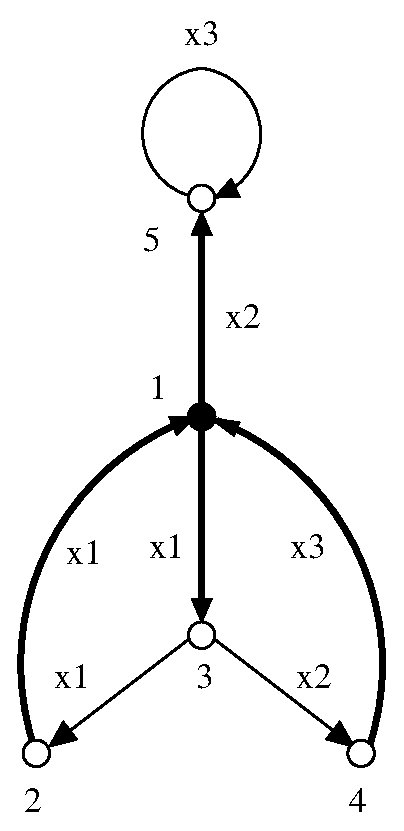
\includegraphics[scale=.52]{stallh1.eps}
\caption{Stallings automaton $\G_{A_1}$ for $H_1$}
\label{fig:stall1}
\end{subfigure}
\hspace{5mm}
\begin{subfigure}[b]{.25\columnwidth}
\psfrag{a}{$(1,2)$}
\psfrag{b}{$(2,3)$}
\psfrag{c}{$(3,1)$}
\psfrag{d}{$(4,5)$}
\psfrag{e}{$(1,5)$}
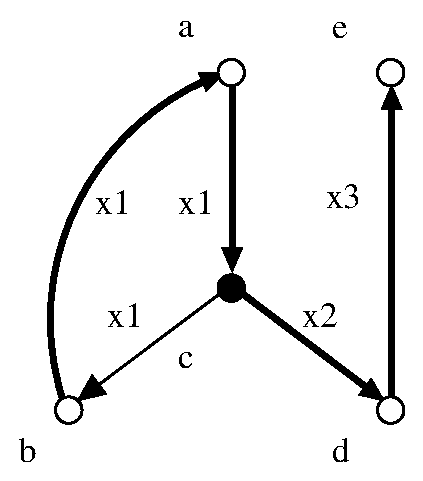
\includegraphics[scale=.52]{GxG-1.eps}
\caption{$\G_{A_1}\times \G_{A_1}$: connected component of $(3,1)$}
\label{fig:GxG-1}
\end{subfigure}
\hspace{5mm}
\begin{subfigure}[b]{.25\columnwidth}
\psfrag{a}{$(2,1)$}
\psfrag{b}{$(3,2)$}
\psfrag{c}{$(1,3)$}
\psfrag{d}{$(5,4)$}
\psfrag{e}{$(5,1)$}
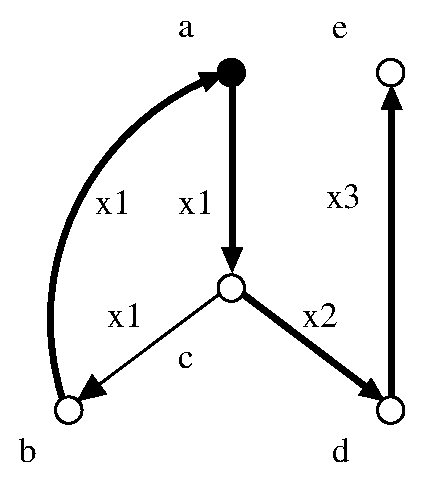
\includegraphics[scale=.52]{GxG-2.eps}
\caption{$\G_{A_1}\times \G_{A_1}$: connected component of $(2,1)$}
\label{fig:GxG-2}
\end{subfigure}
\end{center}
\caption{Example \ref{ex:f_1}.}\label{fig:stall}
\end{figure}

\begin{example}\label{ex:f_2}
Let $F_2$ be the free group on generators
$y_1,y_2,y_3,y_4$ with the subgroup $H_2 = \la h_1^{\prime},
h_2^{\prime},h_3^{\prime}\ra$, where
$h_1^{\prime}=y_2^2$,
$h_2^{\prime}=y_3y_4$ and
$h_3^{\prime}=y_1^2y_3y_1^{-1}y_2$.
The Stallings automata, $\G_{A_2}$ for $H_2$,
with maximal subtree $T_2$ highlighted and base vertex $1$, is shown
in Figure \ref{fig:stallh2}.
The set $L_{T_2}$ corresponding to the maximal subtree  $T_2$ is
 $L_{T_2}=
\{1, y_1, y_1^2,
y_2^{-1}, y_2^{-1}y_1, y_3 \}$.
Let the set of double coset representatives for $H_2$ be $S_2=S_2^{(1)}
\cup S_2^{(2)}$.

To find the normal form of $f_1^\prime=y_1^2y_3y_1^{-1}y_2y_3y_4y_1y_2
y_3y_4y_2^2$: use ${A_2}$ to read off the maximal acceptable
prefix $h= y_1^2y_3y_1^{-1}y_2y_3y_4=h_3^\prime h_2^\prime$ of $f_1^\prime$; and  the maximal
$L_{Q_2}$-prefix $p=y_1$ of the rest of $f_1^\prime$.  Next $q^{-1}=
y_2^{-2}y_4^{-1}y_3^{-1}y_2^{-1}$, so $g=y_2^{-2}y_4^{-1}y_3^{-1}
=h_1^{\prime -1}h_2^{\prime -1}$
and $t=y_2^{-1}$. This element will be represented by an element
of $S_2^{(2)}$, so we need to construct $\G_{A_2}\times \G_{A_2}$.
There are $7$  non-trivial, non-diagonal components. One is shown
in Figure \ref{fig:G2xG2-1} and the remaining
six in Figure \ref{fig:G2xG2-2}. In all cases the solid vertex
corresponds to the $\sim$ representative and connecting elements
are paths in the highlighted trees. Following Algorithm I, the
normal form of $f_1^\prime$ is 
\[f_1^\prime=h yz^{-1} g^{-1},\]
where $y=y_1$, $z=y_2$ and $yz^{-1}=y_1y_2^{-1}\in S_2^{(2)}$: that is
\[f_1^\prime=h^\prime_3h_2^\prime y_1y_2^{-1} (h_1^\prime)^{-1}(h_2^\prime)^{-1}.\]
\end{example}
\begin{figure}
\begin{center}

\psfrag{y1}{$y_1$}

\psfrag{y2}{$y_2$}

\psfrag{y3}{$y_3$}

\psfrag{y4}{$y_4$}
\psfrag{1}{$1$}
\psfrag{2}{$2$}
\psfrag{3}{$3$}
\psfrag{4}{$4$}
\psfrag{5}{$5$}
\psfrag{6}{$6$}
\begin{subfigure}[b]{.3\columnwidth}
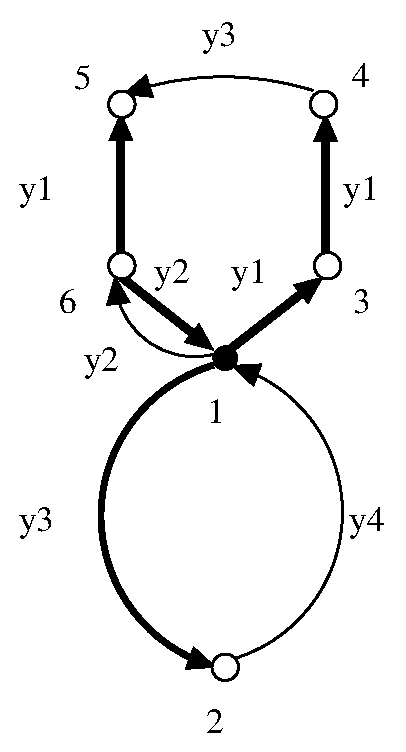
\includegraphics[scale=.52]{stallh2.eps}
\caption{Stallings automaton $A_2$ for $H_2$}
\label{fig:stallh2}
\end{subfigure}
\hspace{25mm}
\begin{subfigure}[b]{.3\columnwidth}
\psfrag{a}{$(5,3)$}
\psfrag{b}{$(6,1)$}
\psfrag{c}{$(1,6)$}
\psfrag{d}{$(3,5)$}
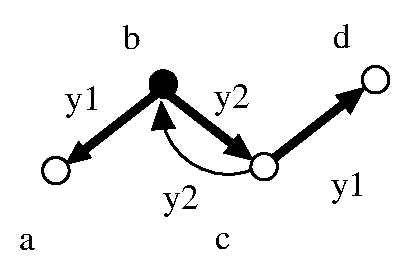
\includegraphics[scale=.52]{G2xG2-1.eps}
\caption{$\G_{A_2}\times \G_{A_2}$: connected component of $(6,1)$}
\label{fig:G2xG2-1}
\end{subfigure}
\end{center}
\caption{Stallings automata for Example \ref{ex:f_2}.}\label{fig:stallagain}
\end{figure}
\begin{figure}
\begin{center}

\psfrag{y1}{$y_1$}

\psfrag{y2}{$y_2$}

\psfrag{y3}{$y_3$}

\psfrag{y4}{$y_4$}
\psfrag{b}{$(1,3)$}
\psfrag{c}{$(3,4)$}
\begin{subfigure}[b]{.13\columnwidth}
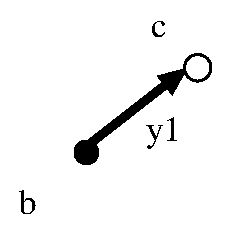
\includegraphics[scale=.5]{G2xG2-2.eps}
\caption{$(1,3)$}
\label{fig:G2xG2-2-1}
\end{subfigure}
\hspace{1mm}
\begin{subfigure}[b]{.13\columnwidth}
\psfrag{b}{$(3,1)$}
\psfrag{c}{$(4,3)$}
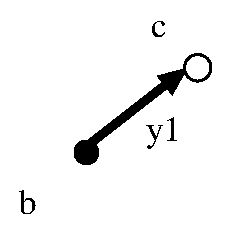
\includegraphics[scale=.5]{G2xG2-2.eps}
\caption{$(3,1)$}
\label{fig:G2xG2-2-2}
\end{subfigure}
\hspace{1mm}
\begin{subfigure}[b]{.13\columnwidth}
\psfrag{y1}{$y_3$}
\psfrag{b}{$(1,4)$}
\psfrag{c}{$(2,5)$}
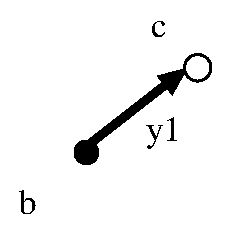
\includegraphics[scale=.5]{G2xG2-2.eps}
\caption{$(2,5)$}
\label{fig:G2xG2-2-3}
\end{subfigure}
\hspace{1mm}
\begin{subfigure}[b]{.13\columnwidth}
\psfrag{y1}{$y_3$}
\psfrag{b}{$(4,1)$}
\psfrag{c}{$(5,2)$}
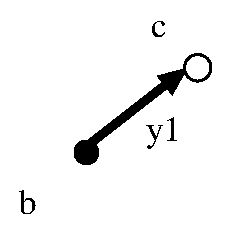
\includegraphics[scale=.5]{G2xG2-2.eps}
\caption{$(5,2)$}
\label{fig:G2xG2-2-4}
\end{subfigure}
\hspace{1mm}
\begin{subfigure}[b]{.13\columnwidth}
\psfrag{y1}{$y_1$}
\psfrag{b}{$(3,6)$}
\psfrag{c}{$(4,5)$}
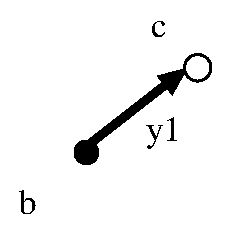
\includegraphics[scale=.5]{G2xG2-2.eps}
\caption{$(4,5)$}
\label{fig:G2xG2-2-5}
\end{subfigure}
\hspace{1mm}
\begin{subfigure}[b]{.13\columnwidth}
\psfrag{b}{$(6,3)$}
\psfrag{c}{$(5,4)$}
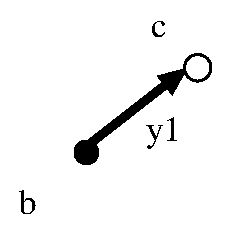
\includegraphics[scale=.5]{G2xG2-2.eps}
\caption{$(6,3)$}
\label{fig:G2xG2-2-6}
\end{subfigure}
\end{center}
\caption{Example \ref{ex:f_2}: connected components of $\G_{A_2}\times \G_{A_2}$.}\label{fig:G2xG2-2}
\end{figure}

In fact if we don't require uniqueness of representatives then
there is a much simpler algorithm to write words in normal form.
This simply finds the maximal prefix $h_1$ of $w$  accepted  by
$A$  and so $w=h_1\circ v$. It then finds the maximal prefix $p$
of $v^{-1}$ accepted by $A$. Setting $h_2=p^{-1}$ gives
$w=h_1\circ d \circ h_2$, for some uniquely determined word $d$,
which is a (non-unique) double coset representative.

%%
%%
%%As before let $g$ be a word in $F_1\ast F_2$ and suppose that
%%$g=g_1\cdots g_t$ in reduced form. Denote $S= S_1 \cup S_2$, where
%%$S_1$ are sets of double coset representatives for $H_1$ and $H_2$
%%correspondingly. Write each syllable $g_i$ of $g=g_1\cdots g_t$ in
%%normal form using the algorithm above. This gives
%%$g_i=h_{i,1}d_ih_{i,2}$, with $d_i\in S$ and $h_{i,j}\in H_1\cup
%%H_2$. Using $\phi_1^{-1}$ or $\phi_2^{-1}$, as appropriate, we now
%%write $h_{i,1}$ and $h_{i,2}$ as reduced words in $\FF(Z)$. For
%%$i=1,\ldots , t-1$, we reduce the word $h_{i,2}h_{(i+1),1}\in
%%\FF(Z)$ to give a reduced word $h_i\in \FF(Z)$ and set $h_0=h_{1,1}$
%%and  $h_{t+1}=h_{t,2}$. Then $g$ has normal form $h_0d_1h_1\cdots
%%d_th_{t+1}$.
%%
%%
%%\begin{example}\label{ex:g}
%%Let $g =f_1 f_2 f_1^{-1}$ in settings of Example \ref{ex:f_1f_2}.
%%Set $z_i = h_i = h_i^{\prime}$ for $i= 1,2,3$; then
%%
%%\begin{align*}
%%g &= (z_2^2z_1)\cdot x_1 \circ x_3^3x_1^{-1} \circ x_1^{-1}\cdot
%%(z_3^{-1}z_3^2z_2) \cdot y_1 \circ (y_2^{-1})^{-1}\\ &\cdot(z_2 z_1 z_3)\cdot x_1\circ x_1 x_3^{-3} \circ x_1^{-1}\cdot (z_1^{-1}z_2^{-2})=\\
%%&(z_2^2z_1)\cdot d_1(x) \cdot (z_3z_2) \cdot d_2(y) \cdot(z_2 z_1
%%z_3) \cdot d_1(x)^{-1} (z_1^{-1}z_2^{-2}).
%%\end{align*}
%%
%%
%%
%%\end{example}

%
%%%
%
%%%%%%%%%%%%%%%%%%%%%%%%%%%%%%%%%%%%%%%%%%%%%%%%%
\section{The generalised folding process}\label{sec:foldings}

Recall from above that $F_1$ and $F_2$ are free groups on finite sets
$X_1$ and $X_2$, respectively;
 $H_1 \leq F_1$ and $H_2 \leq F_2$ are subgroups of rank $m$, freely 
generated by $\{h_1,\ldots, h_m\}$ and $\{h_1^\prime,\ldots ,h_m^\prime\}$. 
The isomorphism from $H_1$ to $H_2$ which maps $h_i$ to $h_i^\prime$ is 
denoted $\phi$.

Now let 
$Z=\{z_1,\ldots, z_m\}$ be a set disjoint from $X_1\cup X_2$. Then there
is an isomorphism $\phi_1:\FF(Z)\maps H_1$, such that $\phi_1(z_i)=h_i$,
 and an isomorphism $\phi_2:\FF(Z)\maps H_2$, such that $\phi_2(z_i)
=h_i^\prime$, $i=1,\ldots, m$. 
 Let $G$ to be the free product with amalgamation: 
${G = F_1 \underset{H_1=H_2}{\ast} F_2}$.  Then $G$ has a 
 presentation  
\[\la X_1\cup X_2\cup Z  | h_i =z_i= h_i', i=1 \ldots m\ra.\] 

\begin{definition}\label{def:dcnf}  
 Let $S_1$ and $S_2$ be sets of  double coset representatives for 
$H_1\le F_1$ and $H_2\le F_2$, respectively. 
A word $w\in \FF(X_1\cup X_2\cup Z)$ is in 
\emph{double coset normal form} (or \emph{dc-normal form}) if
$w = h_{0}p_1h_{1}p_2 \cdots h_{k-1}p_kh_{{k}}$, $k\ge 0$,   where for $i=1,\ldots, k$,  
\be[(a)] 
\item $h_i$ is a reduced word in $\FF(Z)$, for $i=0,\ldots, k$; 
\item  $p_i  \in S_1\cup S_2$ and $p_i\neq 1$, for $i=1,\ldots, k$,  and 
\item if  $p_i\in S_j$ then $p_{i+1}\notin S_j$, $j\in \{1,2\}$.
\ee
\end{definition}
From now on when we say ``normal form'' we mean ``double coset normal form'' unless 
we explicitly say something to the contrary.
\begin{theorem}\label{thm:dcnf}
Every element of $G$ is represented by a unique element of 
$\FF(X_1\cup X_2\cup Z)$ in double coset normal form.
\end{theorem} 
\begin{proof}
To see that every $g\in G$ can be written in dc-normal form, first
write $g$ in reduced form; say $g=f_1\cdots f_t$, where $f_i$ is in a
factor. Assuming that $f_i\in F_j$, let $a_is_ib_i$ 
be the double coset representative of $f_i$, so
$a_i,b_i\in H_j$ and $s_i\in S_j$. Let $z^{\prime}_i=\phi_j^{-1}(a_i)$ and 
$z^{\prime\prime}_i=\phi_j^{-1}(b_i)$. Repeat this for $i=1,\ldots ,t$ and then
let $z_i$ be the free reduction of $z^{\prime}_iz^{\prime\prime}_{i+1}$, 
for $i=1,\ldots ,t-1$. Setting $z_0=z^{\prime}_1$ and $z_t=
z^{\prime\prime}_t$, it follows that 
\[z_0s_1z_1\cdots z_{t-1}s_tz_t\]
is a dc-normal form for $g$. 

Now suppose that $w$ and $w^\prime$ are words in dc-normal form and that 
$w=_G w^\prime$. Let $w=h_{0}p_1h_{1}p_2 \cdots h_{k-1}p_kh_{{k}}$,
and $w^\prime =h_{0}^\prime p_1^\prime h_{1}^\prime  p_2^\prime 
\cdots h_{k-1}^\prime p_k^\prime h_{{k^\prime}}^\prime$, where 
$h_i, h_i^\prime\in \FF(Z)$ and $p_i,p_i^\prime\in S_1\cup S_2$.
 For fixed $i\ge 2$, assuming that $p_i\in F_j$, let $f_i=p_i\phi_j(h_i)$. 
Similarly let $f_1=\phi_j(h_0)p_1\phi_j(h_1)$. Then $f_1\cdots f_k$, is 
a reduced form for the element $w_1\in G$. Similarly, we obtain a reduced
form $f_1^\prime \cdots f_{k^\prime}^\prime$ for $w^\prime$. 
If $k=0$ then we may assume $w=_G f_1=\phi_1(h_0)\in H_j$, 
and it follows that $k^\prime =0$ and $w^\prime=_G f_1^\prime=\phi_1(h_1^\prime)\in H_1$. 
As $H_1$ embeds in $G$ this implies that $w=w^\prime$. Thus the result
holds when $k=0$ and we may assume inductively that $k>0$ and the result holds 
for elements represented by normal forms of length less than $k$. 
Comparing reduced forms, we have $k=k^\prime$. 

Moreover, $1=_G =w^\prime w^{-1}= f_1^\prime \cdots f_{k}^\prime
f_k^{-1}\cdots f_1^{-1}$, so by the fundamental theorem for reduced forms,
we have $ f_{k}^\prime f_k^{-1}\in H_j$, for $j=1$, or $2$. Hence, for 
some $a, b\in H_j$ we have $p_k^\prime=a p_k b$. Therefore $p_k^\prime =p_k$,
and now, as $p_k$ is a double coset representative and  $ f_{k}^\prime f_k^{-1}\in H_j$,
it follows that $h_k=h_k^\prime$. Applying the inductive hypothesis to their prefixes of 
length
$2k-1$, we see that $w=w^\prime$, as required.
\end{proof}
The object of this section is to construct an automaton which will accept a word
$w$ in double coset normal form if and only if it belongs to a
given subgroup $K$ of $G$. The idea is to do this by starting with the
flower automaton for the generators of $K$, written in (double
coset) normal form; carrying out Stallings folding as usual to
produce an inverse automaton; and next
adding some additional paths to allow normal forms to be read.
This may introduce new non-determinism in some  states (i.e. edges
which may be folded), so the resulting automaton must be folded
again. The result of the final folding is the candidate automaton.

 Suppose $L$ is the
language accepted by the flower automaton of $K$. The image of $L$ under
the canonical map to $G$ is $K$. All the stages of our generalised folding
process will preserve this image, so our final automaton will accept a language
$L_1$ which also maps to $K$. We must then prove that, if $w$ is a word
in normal form which represents an element of $K$ then $w$ is in $L_1$. It will
therefore suffice to show that, if $u$ is any word in $L_1$ then the
normal form of $u$ is also in $L_1$.

Let $S_1$ and $S_2$ be sets of double coset representatives of 
$H_1\le F_1$ and $H_2\le F_2$, respectively, as constructed in Section 
\ref{sec:dcforms}. 
Denote $S= S_1 \cup S_2$. Let $A_k$ be the
Stallings automaton for $H_k$ and let $T_k$ be a spanning tree for
the associated graph $\G_{A_k}$, $k=1,2$. The alphabet of $A_k$ is
$X_k$ and the set of states of $A_k$ is denoted $Q_k$.

%\subsection{Construction of the double coset normal form}\label{sub:construction_dcnf}}
Suppose that $g \in G$ and $g=g_1\cdots g_t$ is in reduced form.
Write each syllable $g_i$ of $g=g_1\cdots g_t$ in normal form
using the algorithm I above. This gives
$g_i=h_{i,1}d_ih_{i,2}$, with $d_i\in S$ and $h_{i,j}\in H_1\cup
H_2$. Using $\phi_1^{-1}$ or $\phi_2^{-1}$, as appropriate, we now
write $h_{i,1}$ and $h_{i,2}$ as reduced words in $\FF(Z)$. For
$i=1,\ldots , t-1$, we reduce the word $h_{i,2}h_{(i+1),1}\in
\FF(Z)$ to give a reduced word $h_i\in \FF(Z)$ and set $h_0=h_{1,1}$
and  $h_{t+1}=h_{t,2}$. Then $g$ has normal form $h_0d_1h_1\cdots
d_th_{t+1}$.


\begin{example}\label{ex:g}
Let $F_i$ and $H_i$ be given in Examples \ref{ex:f_1} and  
Example \ref{ex:f_2}, and  
let $f_1$ and $f_2$ be the elements of $F_1$ in Example \ref{ex:f_1} and 
$f_1^\prime\in F_2$ as in Example \ref{ex:f_2}. 
Set $z_i = h_i = h_i^{\prime}$ for $i= 1,2,3$. 

Let $g =f_1 f_1^\prime f_2$; then we have 
\begin{align*}
f_1&=(h_2^{2}h_1) x_1x_3x_1 (h_1^{-1}h_3^{-1})\\
&=z_2^2z_1  x_1x_3x_1z_1^{-1}z_3^{-1},\\
f_2&=(h_3^{-1}h_2^{-1}) x_1^{-1}\\
&=z_3^{-1}z_2 x_1^{-1}\textrm{ and }\\
f_1^\prime&=h^\prime_3h_2^\prime y_1y_2^{-1} (h_1^\prime)^{-1}(h_2^\prime)^{-1}\\
&= z_3z_2 y_1y_2^{-1} z_1^{-1}z_2^{-1}.
\end{align*}
Therefore the double coset normal form of $g$ is 
\[g=z_2^2 z_1  x_1 x_3 x_1 z_1^{-1} 
z_2y_1y_2^{-1} z_1^{-1}z_2^{-1}
z_3^{-1}z_2^{-1} x_1^{-1}.
\]
\end{example}



\subsection{Double coset automata}\label{sec:dca}
%
%
Let $K=\la k_1, \ldots , k_s\ra$, where $k_i$ is an element of $G$
written in normal form: say
\begin{equation}\label{eq:k-form}
k_i= h_{i,0}t_{i,1}h_{i,1}\cdots t_{i,m_i}h_{i,m_i+1},
\end{equation}
with $h_{i,j}\in \FF(Z)$ and $t_{i,j}\in S_1\cup S_2$. Denote
by $\hat K$ the subgroup of  $\FF(X_1\cup X_2 \cup Z)$ generated by
$k_1, \ldots , k_s$. Let $\S=(X_1\cup X_2 \cup Z)^{\pm 1}$.
Let $\cF(K)$ be the flower automaton of $\hat K$, and let
$\G$ be the corresponding rooted graph. If $e$ is an edge of $\G$ then
$e$ is labelled by a letter of $\S$
occuring in $h_{i,j}$ or $t_{i,j}$, for some $i,j$, as in
\eqref{eq:k-form}. If $e$ is labelled by a letter of $Z$ we say $e$ has {\em type} $Z$.
 %and define $c(e)=(0,0)$.
If $e$ is labelled by a letter of $X_k$ occuring in $t_{i,j}$, we
say $e$ has {\em type} $X_k$, $k = 1,2$.

Now let $\G_K$ be the Stallings folding of the graph $\G$.  Then
 $\G_K$ is inverse and $\pi(L(\G_K))=K$. However
$L(\G_K)$ does not, in general, contain all normal forms of elements of $K$.
We wish to transform $\G_K$ to allow it to accept normal forms of
elements of $K$. In outline this transformation process consists of
running the loop below, on input $\G_K$,
until it halts, at which point we shall show that we have an
inverse automaton which accepts  normal forms of elements of $K$.
Assume then that $\D_{(0)}$ is an inverse automaton, with alphabet $\S$
and $\pi(L(\D_{(0)}))=K$. \\[1em]
\textbf{Loop.}
Set $n=0$.
\be[Step 1.]
\item\label{it:gf1} Apply Algorithm II below to add new paths to $\D_{(n)}$ which allow normal forms of labels
of certain paths to be read. %If at least one path has been added,
Call the result $\D_{(n)}^{\prime\prime}$.
%If no paths are added at this step,
%halt and output  $\G_K^{(n)}$.
\item\label{it:gf2} Construct the Stallings automaton $\D_{(n+1)}$
of $\D_{(n)}^{\prime\prime}$. If $\D_{(n+1)}$ and
$\D_{(n)}$ have the same
 number of
$X_1$ and $X_2$ components (see below) then output $\D_{(n+1)}$
and stop. Otherwise, add $1$ to $n$ and  repeat Step \ref{it:gf1}.
\ee

Algorithm II below describes exactly how to carry out Step 1 of
this loop. Since Step 1 may run more than once,  the input to this
algorithm is assumed to be an arbitrary inverse automaton $\D$,
with alphabet $\S$ and $\pi(L(\D))=K$. The output of Algorithm II 
is a rooted,
labelled, involutive automaton, with the same alphabet, which may
fail to be deterministic. We shall show that, if we start as above
with $\G_K=\D_{(0)}$,  the loop halts, at some $n<\infty$; at
which point $\D_{(n+1)}$ is an inverse automaton which accepts the
normal form of every element of $K$. \\[1em]

\noindent\textbf{Algorithm II}. \\

Let $\D$ be an inverse automaton, with alphabet $\S$ and
start and final state $1$, such that
$\pi(L(\D))=K$.
For $k=1,2$, let $\D_k$ be the graph formed from $\D$ by removing all edges of
type $X_{k^\prime}$, where $k\neq k^\prime$. An $X_k$ component of
$\D_k$ is the subgraph of $\D$ formed from a connected component
of $\D_k$ by removing all leaves which are incident to edges of
type $Z$, and then repeating the process till there are no such
leaves left. Given an $X_k$ component $\T$ of $\D_k$,  a
{\em boundary vertex} of $\T$ is defined to be a vertex
$\a$ such that $\a$ is incident, in $\D$, to a vertex which does not
belong to $\T$.
 We shall modify each  $X_k$ component $\T$ of $\D_k$ so that if $p$ is a path,
from a  boundary vertex $u$  to a boundary vertex $v$ of $\T$,
then the normal form  of  the label $l(p)$ of $p$ is the label of
a path from $u$ to $v$. Throughout the modification process we
keep track of the boundary vertices, so that once modification is
complete the $X_k$ components can be reassembled, by attaching as
they did in $\D$. The modification of an $X_k$ component $\Theta$
of $\D_k$ consists of
five steps, producing new graphs $\T_1$, $\T_2$, $\T_3$, $\T_4$
and $\T_5$. In each case there is a canonical morphism $\theta_i$
from $\T_{i-1}$ to $\T_i$ and,
 (writing $\T=\T_0$)
we define the {\em boundary vertices} of $\T_{i}$ to be the vertices $\theta_{i}(v)$
of $\T_i$, such that $v$ is a boundary vertex of $\T_{i-1}$. Moreover the
 images $\theta_i\circ \cdots\circ \theta_1(v)$ of vertices of $\T$ in $\T_i$ 
will be referred to as  {\em vertices of} $\T$.


The modification process is followed by a ``reassembly'' phase, in which
we reconnect the $X_k$ components of $\D$, to form the output of the algorithm.
\\[1em]

\noindent\textbf{Modification 1: $\T\leadsto \T_1$.}\\
This step involves the addition of paths labeled by $X_k$-words corresponding to
$z$-edges of an $X_k$ component.

Let $\T$ be an $X_k$ component of $\D_k$. If $(\a,z,\b)$ is an
edge of $\T$ labelled by an element $z\in Z$ then add a path from
$\a$ to $\b$ labelled by $\phi_k(z)$ to the graph $\T$. Do this
for all such edges and call the result
$\T_1^\prime$. Fold $\T_1^\prime$ to form the graph 
$\T_1$. (See Figure \ref{fig:alg2-1}.)
\begin{figure}
\begin{center}
\psfrag{a}{$\a$}
\psfrag{b}{$\b$}
\psfrag{h}{$z$}
\psfrag{w}{$w$}
\begin{subfigure}[b]{.25\columnwidth}
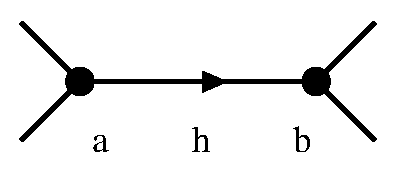
\includegraphics[scale=.5]{alg2-1a.eps}
\label{fig:alg2-1a}
%\caption{}
\end{subfigure}
\raisebox{3ex}{$\leadsto$}
\begin{subfigure}[b]{.25\columnwidth}
\psfrag{a}{$\a$}
\psfrag{b}{$\b$}
\psfrag{h}{$z$}
\psfrag{w}{$w$}
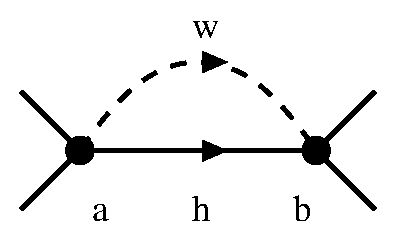
\includegraphics[scale=.5]{alg2-1b.eps}
\label{fig:alg2-1b}
%\caption{}
\end{subfigure}
\end{center}
\caption{$\Theta$ to $\Theta_1$: $w=\phi_k(z)$.}\label{fig:alg2-1}
\end{figure}
Let $\theta_1$ be the canonical morphism from $\Theta$ to
$\Theta_1$. If $\a$ and $\b$ are vertices of $\Theta$ then, 
since $\theta$ is a morphism 
$\pi(L(\Theta, \a,\b))\subseteq \pi(L(\Theta_1,\theta(\a),\theta(\b)))$. 
On the other hand if $w$ is in  $L(\Theta_1,\theta(\a),\theta(\b))$
then, since $\Theta_1$ is a folding of $\Theta_1^\prime$,
 there is a path labelled $w^\prime$ from $\a$ to $\b$ in $\Theta_1^\prime$,
such that $\pi(w^\prime)=\pi(w)$. 
By construction then there exists  a path $w^{\prime\prime}$ from
$\a$ to $\b$ in $\Theta$, such that $\pi(w^{\prime\prime}) =
\pi(w^\prime)$. Hence $\pi(L(\Theta_1,\theta(\a),\theta(\b)))
= \pi(L(\Theta, \a,\b))$.  \\[1em]
\begin{comment}
and  define the boundary vertices of $\T_1$ to be the
vertices $\theta_1(v)$ of $\T_1$, such that $v$ is a boundary
vertex of $\T$. (We shall not mention this again in later
steps.) \\[1em]
%%%
As $\pi(a)=\pi(wb)\in G$, if $L_3$ and $L_3^\prime$ are the languages
accepted by $(\T_3,\a,\b)$ and $(\T_3^\prime,\a,\b)$, for some
vertices $\a,\b$ of $\T$, then $\pi(L_3)=\pi(L_3^\prime)$.
Repeat this process for all pairs of  vertices which are not
covered by $\cP_3$  and fold
the result to form the graph $\T_4$. Again there is a natural
morphism $\theta_4$ from $\T_3$ to $\T_4$ and
we have $\pi(L_3)=\pi(L_4)$, in the same notation as in previous cases.
\end{comment}
%%%

\noindent\textbf{Modification 2: $\T_1\leadsto \T_2$.}\\
Here we add to $\T_1$ paths labelled by $\phi_k^{-1}$ images of labels of simple
paths in $\T_1\times \G_{A_k}$, from $(\a_i,1)$ to $(\a_j,1)$; for 
appropriate $i,j$. 
 Let $\cP_1=\T_1\times \G_{A_k}$. Then there is a path
 labelled $w$ from $\a$ to $\b$
in $\T_1$ and a path labelled $w$ from $\a^\prime $
to $\b^\prime$ in $\G_{A_k}$ if and only if there is a path
labelled $w$ from $(\a,\a^\prime)$ to $(\b,\b^\prime)$ in $\cP_1$.
 We shall
use this property of $\cP_1$ to determine which new paths to add  to
$\T_1$. Choose a spanning  forest $\U_1$ of  $\cP_1$. Next
 order the vertices of
$\T_1$: say these are $\a_0,\ldots, \a_t$, in the order written.

Let $\a_i$, $\a_j$ be vertices of  $\T$  with $i\le j$. If
\begin{itemize}
\item
 there
exists a simple path $p$ in $\cP_1$ from $(\a_i,1)$ to $(\a_j,1)$ and
\item 
$p$ does not contain a vertex $(\a_k,1)$ with $k\in\{i,j\}$
\end{itemize}
then let $l_p\in \FF(X_k)$ be the label of $p$ and let
$w_p=\phi_k^{-1}(l_p)\in \FF(Z)$. Let $q$ be a path (disjoint from
$\T_1$) of length $|w_p|$ and with label $w_p$. Identify the
initial vertex of $q$ with $\a_i$ and the terminal vertex of $q$
with $\a_j$. (See Figure \ref{fig:alg2-2}.)
\begin{figure}
\begin{center}
\psfrag{a}{$\a$}
\psfrag{b}{$\b$}
\psfrag{h}{$l_p$}
\psfrag{w}{$w_p$}
\psfrag{ai}{$(\a_i,1)$}
\psfrag{bi}{$(\a_j,1)$}
\psfrag{1}{$1$}
\psfrag{Th1 to Th2}{$\T_1\leadsto \T_2$}
\psfrag{cP}{$\cP_1$}
\psfrag{G_A}{$\G_{A_k}$}
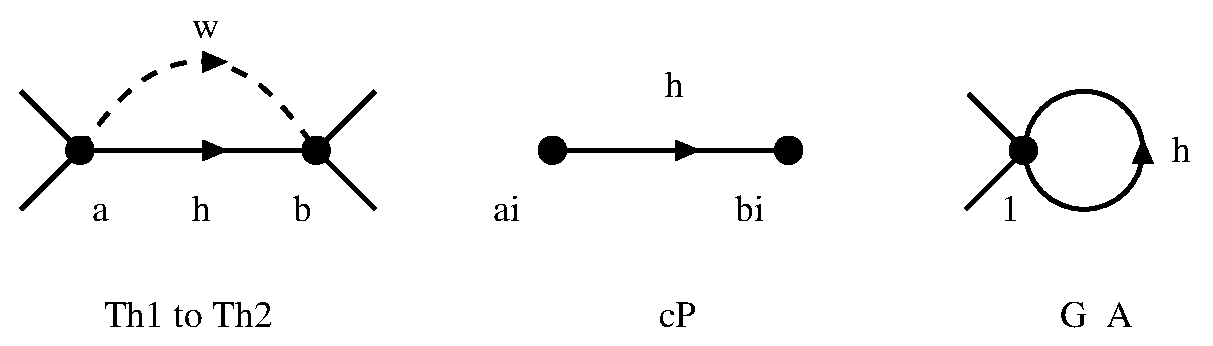
\includegraphics[scale=.5]{alg2-2.eps}
\end{center}
\caption{$\Theta_1$ to $\Theta_2$: $w_p=\phi_k^{-1}(l_p)$.}\label{fig:alg2-2}
\end{figure}
Repeat this process for all simple paths from  $(\a_i,1)$ to
$(\a_j,1)$, over all pairs of vertices $\a_i$, $\a_j$ of $\T$,
with $i\le j$. There are finitely many simple paths in $\cP_1$ so
this process terminates. Call the result $\T_2^\prime$. Then
$\T_1$ is a subgraph of $\T_2^\prime$. Now fold $\T_2^\prime$ to
give a new graph $\T_2$. The composition $\theta_2$ of the the
embedding map of $\T_1$ into $\T_2^\prime$ with the canonical
morphism from $\T_2^\prime$ to $\T_2$ is a morphism from $\T_1$ to
$\T_2$.
 Moreover, if $\a$ and
 $\b$ are
%boundary 
 vertices of $\T_1$ and 
a path $q$ from $\a$ to $\b$, with label $w_p$, is added to $\Theta_1$ 
in forming $\Theta_2$, then there is a path $p$ in $\Theta_1$ with
$\pi(l(p))=\pi(w_p)$. Thus the argument of the previous case shows that  
$\pi(L(\T_1,\a,\b))=\pi(L(\T_2,\theta_2(\a),\theta_2(\b)))$.\\[1em]

\noindent\textbf{Modification 3: $\T_2\leadsto \T_3$.}\\
At this stage we add $\phi_k^{-1}$ images of paths in $\T_2\times
\G_{A_k}$ related to edges of this graph which do not belong to
its spanning subforest and which project to closed paths,
based at $1$, in $\G_{A_k}$.

As the edges added to $\T_1$ to form $\T_2$ are all labelled by elements
of $Z$, and all edges of $\G_{A_k}$ are labelled by elements of $X_k$
the graphs $\cP_1=\T_1\times \G_{A_k}$ and $\cP_2=\T_2\times \G_{A_k}$ differ only
in that the second may have some new isolated vertices. Therefore we may
choose a spanning forest $\U_2$ of $\cP_2$ consisting of the spanning
forest $\U_1$ of $\cP_1$ with some new isolated vertices if necessary.
If $\cP_2$ is a forest then
$\cP_2=\U_2$, there is nothing to do at the
this stage, and we immediately set $\T_3=\T_2$. Otherwise, suppose
that $e$ is an edge of $\cP_2$ which does not belong to $\U_2$ but
which does belong to a component $\Xi$  of $\cP_2$ containing a
vertex $(\a,1)$, for some vertex $\a$ of $\T$. Let $(\a,1)$ be
such a vertex and let $e=((\a_i,\b_1), x, (\a_j,\b_2))$ be an edge
in the same component of $\cP_2$ as $(\a,1)$,
 with label $x$ in $X_k$.
%Let
%$\a_m$ be the minimal vertex of $\T_2$ (necessarily also a vertex
%of $\T_1$)  such that $(\a_m,1)$ belongs to $\Xi$.
 Let $p_i$ be
the path in $\U_2$ from $(\a,1)$ to $(\a_i,\b_1)$ and let $p_j$ be
the path in $\U_2 $ from  $(\a_j,\b_2)$ to $(\a,1)$ and let $l_i$
and $l_j$ be the labels of $p_i$ and $p_j$, respectively. Then
$p_i,e,p_j$ projects to a closed path in $\G_{A_k}$, based at $1$,
with label $h_e=l_i x l_j \in H_k\subseteq F_k$. Moreover
$p_i,e,p_j$ projects to a closed path in $\T_2$, based at $\a$,
also with label $h_e$. Let $w_e=\phi_k^{-1}(h_e) \in \FF(Z)$ and let
$q$ be a path (disjoint from $\T_2$) of length $|w_e|$ and with
label $w_e$. Identify the initial and terminal vertices of $q$ to
the vertex  $\a$ of $\Theta_2$. (See Figure \ref{fig:alg2-3}.)
\begin{figure}
\begin{center}
\psfrag{a}{$\a$} \psfrag{b}{$\b$} \psfrag{x}{$x$}
\psfrag{h}{$h_e$} \psfrag{w}{$w_e$} \psfrag{li}{$l_i$}
\psfrag{lj}{$l_j$} \psfrag{ai}{$(\a_i,\b_1)$}
\psfrag{bi}{$(\a_j,\b_2)$} \psfrag{(a,1)}{$(\a,1)$}
\psfrag{1}{$1$} \psfrag{Th2 to Th3}{$\T_2\leadsto \T_3$}
\psfrag{cP}{$\cP_2$} \psfrag{G_A}{$\G_{A_k}$}
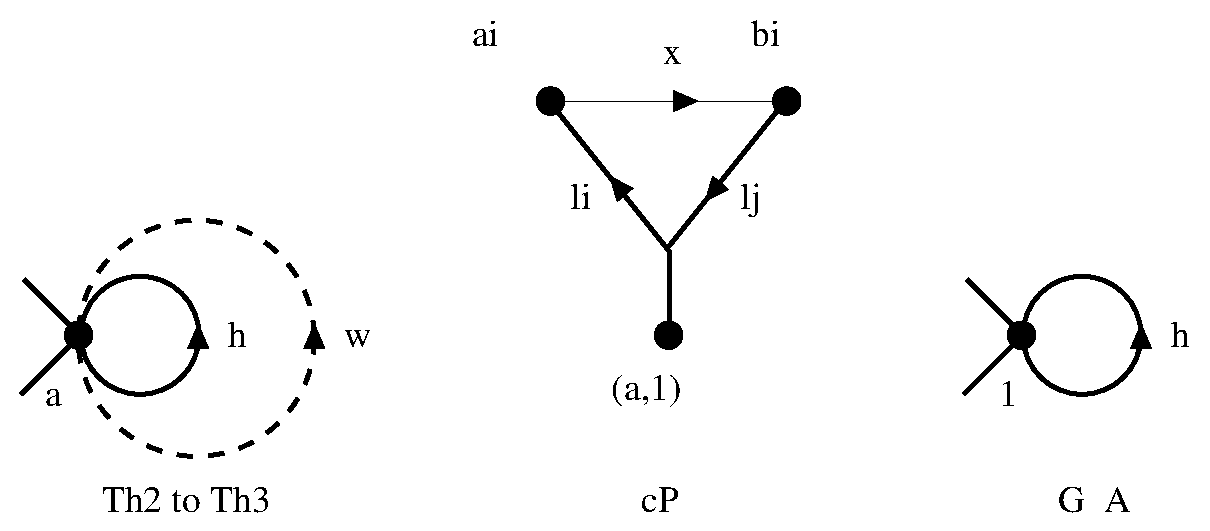
\includegraphics[scale=.5]{alg2-3.eps}
\end{center}
\caption{$\Theta_2$ to $\Theta_3$: $h_e=l_ixl_j$,
$w_e=\phi_k^{-1}(h_e)$.}\label{fig:alg2-3}
\end{figure}
Repeat this process for all such edges $e$ and vertices $(\a,1)$
of $\cP_2$,  fold the resulting graph, and denote the result by
$\T_3$. (In practice it's not necessary to repeat this process for
{\em all} such vertices $(\a,1)$ in $\Xi$: but it makes some
arguments  later easier if we assume that we do so.) As in the
previous case there is a natural morphism $\theta_3$ from $\T_2$
to $\T_3$. Again, if $q$ is a path added to $\Theta_2$ in forming 
$\T_3$ then there is a path $p$ in $\T_2$, with the same end points
as $q$, such that $\pi(l(p))=\pi(l(q))$. Hence, as before, for all
vertices   $\a$, $\b$ of $\T_2$,  
$\pi(L(\T_2,\a,\b))=\pi(L(\T_3, \theta_3(\a),\theta_3(\b)))$.\\[1em]

\noindent\textbf{Modification 4: $\T_3\leadsto \T_4$.}\\
Next we wish to add paths to $\T_3$ that allow us to read the normal
forms of words $w$ which are readable by $\T_3$ and readable,
but not accepted, by $\G_{A_k}$.
 Let
$\cP_3=\T_3\times \G_{A_k}$.
As before we may choose a spanning forest $\U_3$ of $\cP_3$ which
consists of $\U_2$ and some additional isolated vertices.

Recall that we have fixed a spanning subtree
$T_k$ of $\G_{A_k}$.
Let $\d=(\a_j,\b)$ be a vertex of $\cP_3$, with $\b\neq 1$, which lies
in a connected component of $\cP_3$ containing a vertex  $\g=(\a_i,1)$,
for some vertices $\a_i$ and $\a_j$ of $\T$.
Let $b$ be the label of the path in $T_k$ from $1$ to $\b$.
 If $\cP_3$ contains a simple
path from $(\a_i,1)$ to $(\a_j,\b)$, with label $b$,  then
 say that $\cP_3$ {\em covers} the pair $\g,\d$.
If all such pairs of vertices are covered by $\cP_3$ then set $\T_4=\T_3$.
Otherwise
let $p$ be the simple path in $\U_3$ from a
vertex $\g=(\a_i,1)$ to a vertex $\d=(\a_j,\b)$, where $\g,\d$
is not covered by $\cP_3$.
 Let
$p$ have label $a$.
Then $ab^{-1}=h\in H_k$. Let
$w=\phi_{k}^{-1}(ab^{-1})
\in \FF(Z)$ and let $q$ be a path (disjoint from $\T_3$)
with label $wb$. Identify the initial
and terminal vertices of $q$ with vertices $\a_i$ and $\a_j$ of $\T_3$,
respectively, to form a new graph $\T_3^\prime$.
(See Figure \ref{fig:alg2-4}.)
\begin{figure}
\begin{center}
\psfrag{ai}{$\a_i$}
\psfrag{bi}{$\a_j$}
\psfrag{g}{$a$}
\psfrag{h}{$b$}
\psfrag{w}{$wb$}
\psfrag{(ai,1)}{$(\a_i,1)$}
\psfrag{(aj,b)}{$(\a_j,\b)$}
\psfrag{1}{$1$}
\psfrag{b}{$\b$}
\psfrag{Th3 to Th4}{$\T_3\leadsto \T_4$}
\psfrag{U3 in cP}{$\U_3\subseteq \cP_3$}
\psfrag{Tk in G_A}{$T_k\subseteq \G_{A_k}$}
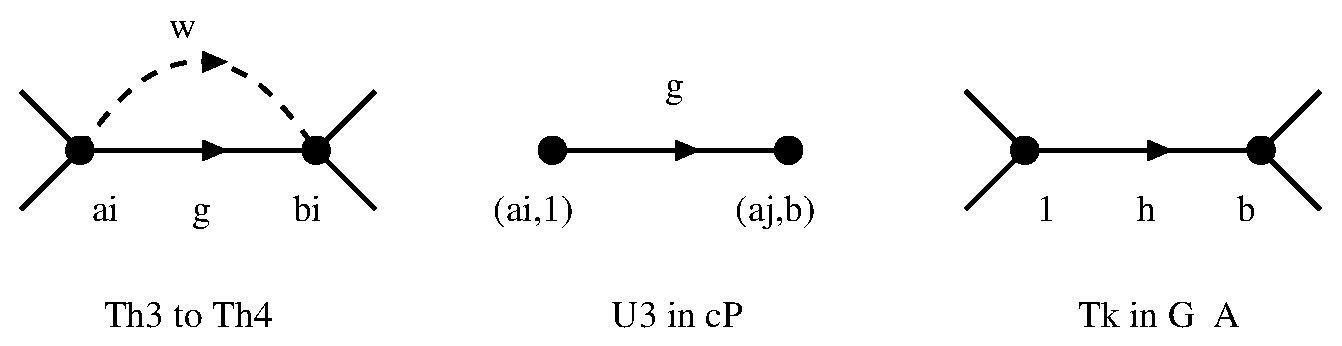
\includegraphics[scale=.5]{alg2-4.eps}
\end{center}
\caption{$\Theta_3$ to $\Theta_4$: $w=\phi_k^{-1}(ab^{-1})$.}\label{fig:alg2-4}
\end{figure}

As $\pi(a)=\pi(wb)\in G$, if $L_3$ and $L_3^\prime$ are the languages
accepted by $(\T_3,\a,\b)$ and $(\T_3^\prime,\a,\b)$, for some
vertices $\a,\b$ of $\T_3$, then $\pi(L_3)=\pi(L_3^\prime)$.
Repeat this process for all pairs of  vertices which are not
covered by $\cP_3$  and fold
the result to form the graph $\T_4$. Again there is a natural
morphism $\theta_4$ from $\T_3$ to $\T_4$. If $L_4$ is the 
language accepted by $(\T_4,\theta_4(\a),(\b))$, for some 
vertices $\a,\b$ of $\Theta_3$, then   
we have $\pi(L_3)=\pi(L_4)$, as in previous cases.\\[1em]

\noindent\textbf{Modification 5: $\T_4\leadsto \T_5$.}\\
Finally we wish to add paths which allow double coset representatives
of type $2$ to be read.
Let $\cP_4=\T_4\times \G_{A_k}$ and choose a spanning forest $\U_4$ for
$\cP_4$.

Suppose $(\e,\xi)\in P\subseteq V(\G_{A_k}\times \G_{A_k})$ and
that the $\sim$ representative of $(\e,\xi)$ is $(\e_0,\xi_0)$.
Let $b_1=w(\e)$, $b_2=w(\xi)$ (the labels
of paths from $1$ to $\e$ and $1$ to $\xi$ in the
subtree $T_k$ of $\G_{A_k}$). Let $a_1=w(\e_0)$ and $a_2=w(\xi_0)$.
By definition of $\sim$ there are  paths in $\G_{A_k}$,
with label
$c=c(\e,\xi)$, from $\e$ to $\e_0$ and from $\xi$ to $\xi_0$.
Furthermore $h_i=
b_ica_i^{-1}\in H_k$ and $w_i=\phi_k^{-1}(h_i)\in \FF(Z)$, for $i=1,2$.
If there
exist paths $p_1$, with label $b_1$ from $(\a_i,1)$ to $(\b,\e)$,
and $p_2$, with label $b_2$ from
$(\a_l,1)$ to $(\b,\xi)$, in $\U_4$,  then
let $q$ be a path (disjoint from $\T_4$)
with label $w_1 a_1a_2^{-1} w_2^{-1}$,
and identify the initial
and terminal vertices of $q$ with  vertices $\a_i$ and $\a_l$
of $\T_4$, respectively.
(See Figure \ref{fig:alg2-5}.)
\begin{figure}
\begin{center}
\psfrag{1}{$1$}
\psfrag{ai}{$\a_i$}
\psfrag{aj}{$\b$}
\psfrag{al}{$\a_l$}
\psfrag{a1}{$a_1$}
\psfrag{a2}{$a_2$}
\psfrag{b1}{$b_1$}
\psfrag{b2}{$b_2$}
\psfrag{c}{$c$}
\psfrag{w}{$w$}
\psfrag{e}{$\e$}
\psfrag{x}{$\xi$}
\psfrag{e0}{$\e_0$}
\psfrag{x0}{$\xi_0$}
\psfrag{(ai,1)}{$(\a_i,1)$}
\psfrag{(al,1)}{$(\a_l,1)$}
\psfrag{(aj,e)}{$(\b,\e)$}
\psfrag{(aj,x)}{$(\b,\xi)$}
\psfrag{1}{$1$}
\psfrag{b}{$\b$}
\psfrag{Th4 to Th5}{$\T_4\leadsto \T_5$}
\psfrag{U4 in cP}{$\U_4\subseteq \cP_4$}
\psfrag{G_A}{$\G_{A_k}$}
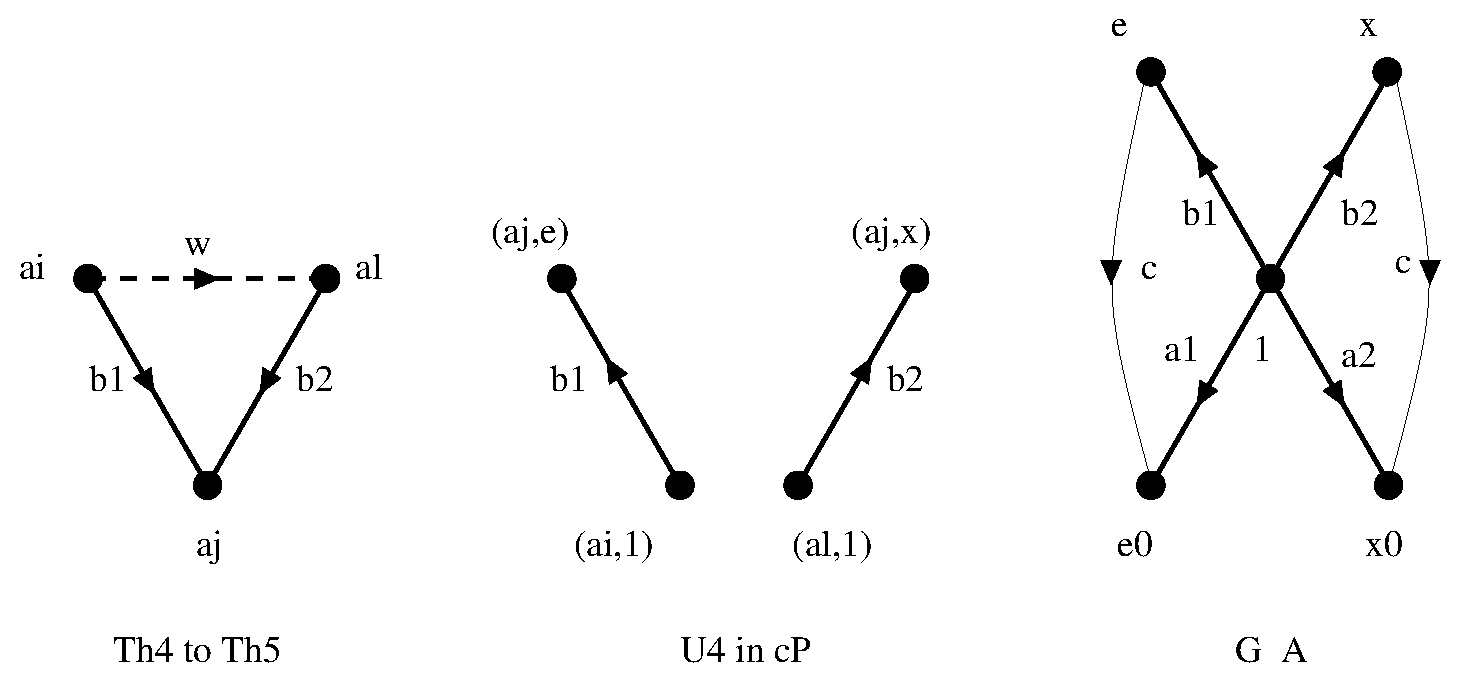
\includegraphics[scale=.5]{alg2-5.eps}
\end{center}
\caption{$\Theta_4$ to $\Theta_5$:
$w=\phi_k^{-1}(b_1ca_1^{-1})a_1a_2^{-1}\phi_k^{-1}(a_2c^{-1}b_2^{-1})$.}
\label{fig:alg2-5}
\end{figure}

Repeat this process for all such paths $p_i$ and $p_j$ and all such
pairs $(\e,\xi)$.
To see that the image of the language accepted by
 the new graph is the same as that of the original note
that the word $b_1b_2^{-1}$ is readable, starting at $\a_i$ and
ending at $\a_l$, in $\T_4$. As $\pi(b_1b_2^{-1})=\pi(w_1a_1a_2^{-1}w_2^{-1})$
the addition of this new path has no effect on the image, under $\pi$, of
the language accepted by the automaton.
 Fold the resulting graph to form $\T_5$. As before, there is 
a natural morphism $\theta_5$ from $\Theta_4$ to $\Theta_5$ and again, 
if $\a,\b$ are
vertices of $\Theta_4$ and $L_4$ and $L_5$ are the languages accepted by 
$(\Theta_4,\a,\b)$ and $(\Theta_5,\theta_4(\a),\theta_4(\b))$, 
respectively, then $\pi(L_4)=\pi(L_5)$.\\[1em]

\noindent\textbf{Reassembly.}\\
The modification process is applied to all $X_k$ components of $\D_k$,
for $k=1$ and $2$. Roughly speaking a new graph is then constructed by
reconnecting the modified $X_k$ components in the same way as they
were connected in $\D$. In detail,
let $\cC$ be the set of all
$X_1$ and $X_2$ components.
Define
\[E_Z=E(\D)\bs \cup_{\Phi\in \cC} E(\Phi)\]
and $\D_Z$ to be the subgraph of $\D$ consisting of all edges
of $E_Z$, and their incident vertices.
Define $\D^\prime$ to be the disjoint union of the
 graphs $\T$, such that $\T\in \cC$, with  the graph $\D_Z$.
Also define $\D^{\prime}_5$ to be the disjoint union of the graphs
$\T_5$, such that $\T\in \cC$, with the graph $\D_Z$. For each
$\T\in \cC$ there is  a morphism
$\theta_5\circ\theta_4\circ\theta_3\circ\theta_2\circ\theta_1$
from $\T$ to $\T_5$. Define $\theta$ to be the morphism from
$\D^\prime$ to $\D^\prime_5$ which consists of the union of these
morphisms with the identity morphism from $\D_Z$ to $\D_Z$. By
construction, for each connected component $\Xi$ of $\D^\prime$
there is an embedding of $\Xi$ into $\D$. Let $\nu$ be the union
of these embeddings over all components of $\D^\prime$.

The output $\D^{\prime\prime}$  of Algorithm II is the quotient of
 $\D^\prime_5$ defined as follows.
Let $u$ and $v$ be vertices in
distinct connected components of $\D^\prime_5$.
\begin{itemize}
\item If $\nu(\theta^{-1}(u))\cap \nu(\theta^{-1}(v))\neq \nul$ then
identify vertices $u$ and $v$. 
For $u \in V(\D^\prime_5)$ let
$[u]$  denote equivalence class of $u$ under the equivalence relation
on $V(\D^\prime_5)$ generated by this identification.
\item 
$\D^{\prime\prime}$ has edge set 
\[\{([u],a,[v]): (u,a,v)\in E(\D^\prime_5)\}.\]
\item The root vertex of $\D^{\prime\prime}$ is the image, in
$\D^{\prime\prime}$, of $\nu^{-1}(1)$, where $1$ is  the root of
$\D$. 
\end{itemize}

\begin{lemma}\label{lem:resol-quot}
Let $[\cdot]$ be the equivalence relation on $V(\D^\prime_5)$
described above. There is a morphism $\rho$ from  $\D$ to
$\D^{\prime\prime}$ given by 
\begin{itemize}
\item 
$\rho(u)=[\theta(\nu^{-1}(u))]$, for
$u\in V(\D)$, and 
\item 
$\rho((u,a,v))=(\rho(u),a,\rho(v))$, for $(u,a,v)\in  E(\D)$. 
\end{itemize}
\end{lemma}
\begin{proof}
First $\rho$ must be shown to be well defined. 
That is, we must verify that $[\theta(\nu^{-1}(u))]$ is a vertex of
$\D^{\prime\prime}$ and that $[\rho(u),a,\rho(v)]$ is an edge. 
If $u \in V(\D)$  
then either $u\in V(\D_Z)$ or  $u$ belongs to
some $X_k$ component of $\D$. Hence
 $\nu^{-1}(u)\neq \nul$. If $u_1, u_2\in \nu^{-1}(u)$, then, 
by definition of
$\D^{\prime\prime}$, $\theta(u_1)$ and $\theta(u_2)$ are equivalent.
Thus $[\theta(\nu^{-1}(u)]$ is a vertex of $\D^{\prime\prime}$,
as required. 
 Suppose that $(u,a,v)$ is an edge
of $\D$ and let $u_1\in \nu^{-1}(u)$ and $v_1\in \nu^{-1}(v)$. Then
$\rho(u)=[\theta(u_1)]$ and $\rho(v)=[\theta(v_1)]$, so 
$[\rho(u), a, \rho(v)]$ is an edge of $\D^{\prime\prime}$. 
Hence $\rho$ is well-defined, and is, moreover, a graph morphism.
\end{proof}


\begin{definition}
Let $\D$ be an inverse automaton.
%, with alphabet $\S$ and
%start and final state $1$, such that
%$\pi(L(\D))=K$.
 The result $\D^{\prime\prime}$ of applying  \ref{it:gf1}
above to $\D$ is called a \emph{double coset resolution} or
\emph{dc-resolution} of $\D$. The graph $\Psi$ obtained by applying
 \ref{it:gf2} to $\D^{\prime\prime}$ is called a \emph{double
coset folding} or \emph{dc-folding} of $\D$.  The composition $\hat\rho$ of
the  morphism
$\rho:\D\maps \D^{\prime\prime}$ with the folding morphism $\D^{\prime\prime}\maps
\Psi$ is called the \emph{dc-folding morphism}.
\end{definition}

\begin{example}\label{ex:K}
Let $F_1=\FF(x_1,x_2,x_3)$ and $H_1=\la h_1,h_2,h_3\ra$, 
as in Example \ref{ex:f_1}, and let $F_2=\FF(y_1,y_2,y_3,y_4)$ and 
$H_2=\la h_1^\prime, h_2^\prime, h_3^\prime\ra$, as in Example \ref{ex:f_2}.
Let $f_1,f_2$ and $f_1^\prime$ be the elements defined in these examples
 and let $G=F_1\ast_{H_1=H_2} F_2$.  

Let  
\[f_3=x_2x_3^{-1}x_1,\, f_4= x_1^4 x_2 x_3 x_1^{-1} x_2^{-1} 
\textrm{ and } f_5=x_1x_2x_3x_2x_3^{-2}x_2^{-1},\]  
and let 
\[ f_2^\prime =y_3y_4y_2^{-1}y_1y_3.\]
Using Algorithm I, the double coset representatives of these elements are
\begin{align*}
f_3 & = x_2x_3^{-1}x_1,\\
f_4 &= h_1h_3 x_1^{-1}x_2^{-1},\\
f_5 &= h_3h_2^{-2}\textrm{ and }\\
f_2^\prime &= h_2^\prime y_2^{-1}y_1y_3.
\end{align*} 

Let $K$ be the subgroup of $G$ generated by $k_1=f_1f_1^\prime f_2$, 
$k_2= f_3f_2^\prime f_4$ and $k_3=f_5$. 
In Example \ref{ex:g} we found the double-coset normal form of
$k_1=g=f_1f_1^\prime f_2$, namely
\[k_1=z_2^2 z_1  x_1 x_3 x_1 z_1^{-1} 
z_2y_1y_2^{-1} z_1^{-1}z_2^{-1}
z_3^{-1}z_2^{-1} x_1^{-1}.\]
The double coset normal forms of $k_2$ and $k_3$ are 
\[k_2=  x_2x_3^{-1}x_1  z_2 y_2^{-1}y_1y_3 z_1z_3 x_1^{-1}x_2^{-1}\]
and 
\[k_3 = z_3z_2^{-2}.\]

We form the flower automaton of $K$ and then its (classical) Stallings folding,
which is 
shown in Figure \ref{fig:Kflower}.
There is one $X_1$ component $\Theta$ of this graph, shown in Figure \ref{fig:KX} 
and two $X_2$ components, $\Theta^\prime$ and $\Theta^{\prime\prime}$, shown in Figure \ref{fig:KY}. Each of these components is input to the loop, in turn.

First consider the $X_1$ component $\Theta$. Modification 1 results in the
graph of Figure \ref{fig:K_f1}. To perform the next stages of the  modification 
process the graph $\Theta_1 \times \G_{A_1}$ is constructed; where $\G_{A_1}$ is the
graph of Example \ref{ex:f_1}, shown in Figure \ref{fig:stall1}. The product graph
is 
shown in Figure \ref{fig:K_f1-x-g}. On examination of $\Theta_1 \times \G_{A_1}$
there is one path to add, from ... to ..., with label $x$, and this gives the
graph $\Theta_2$, shown in Figure \ref{fig:K_f2}.


After performing modifications these  graphs are transformed into
 $\Theta_5$, $\Theta_5^{\prime}$ and $\Theta_5^{\prime\prime}$, shown in Figure \ref{fig:KX5}
The reassembled graph $\Psi$ has the same number of $X_1$ and $X_2$ components as before, so 
the algorithm halts after one iteration of the Loop, outputting the graph of Figure 
\ref{fig:out}. 
\end{example}
\begin{figure}
\begin{center}
\psfrag{a}{$x_1$}
\psfrag{b}{$x_2$}
\psfrag{c}{$x_3$}
\psfrag{r}{$y_1$}
\psfrag{s}{$y_2$}
\psfrag{t}{$y_3$}
\psfrag{x}{$z_1$}
\psfrag{y}{$z_2$}
\psfrag{z}{$z_3$}
\psfrag{u}{$y_4$}
\psfrag{1}{$1$}
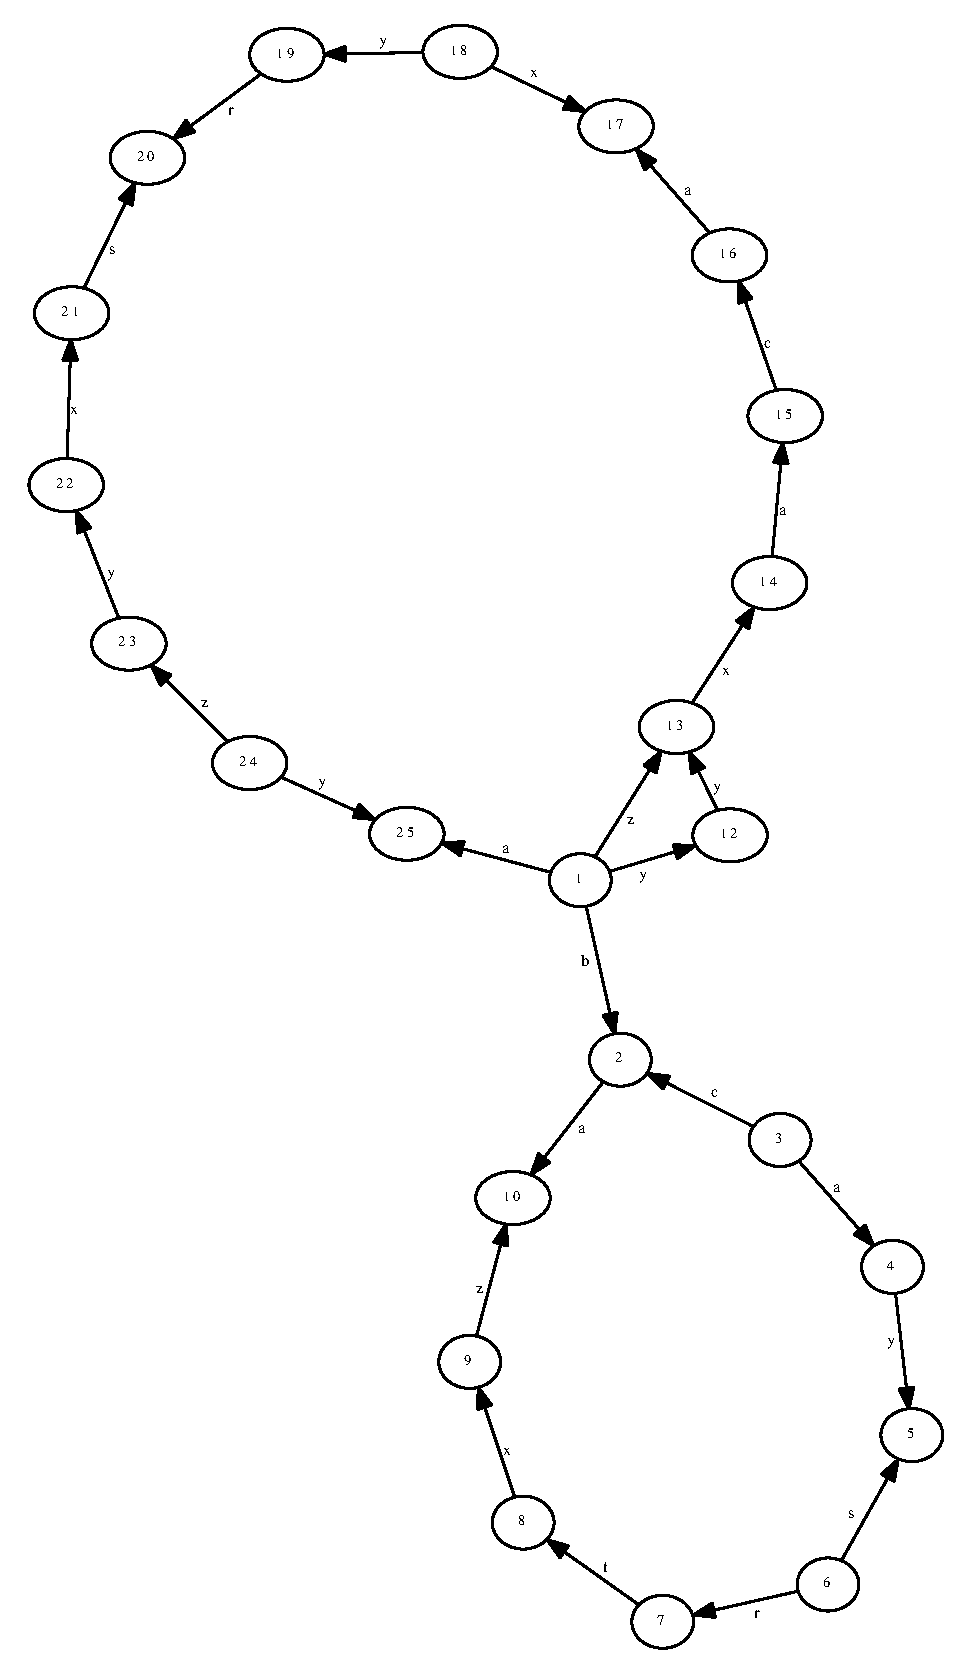
\includegraphics[scale=0.5,bb=0 0 820 720]{python/ex_K_folded.eps}
%\includegraphics[scale=0.4]{python/ex_K.eps}
\caption{The folded flower automaton of $K$}
\label{fig:Kflower}
\end{center}
\end{figure}

\begin{figure}
\begin{center}
\psfrag{a}{$x_1$}
\psfrag{b}{$x_2$}
\psfrag{c}{$x_3$}
\psfrag{r}{$y_1$}
\psfrag{s}{$y_2$}
\psfrag{t}{$y_3$}
\psfrag{x}{$z_1$}
\psfrag{y}{$z_2$}
\psfrag{z}{$z_3$}
\psfrag{u}{$y_4$}
\psfrag{1}{$1$}
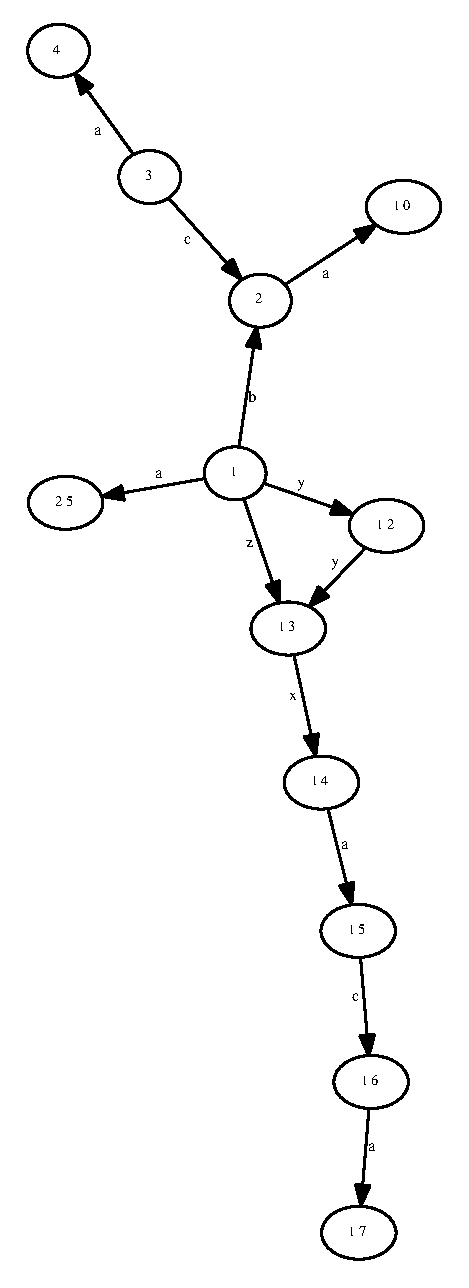
\includegraphics[scale=0.5, angle=90,bb=0 0 300 600]{python/ex_K_X.eps}
\caption{$X_1$ component $\Theta$}
\label{fig:KX}
\end{center}
\end{figure}

\begin{figure}
\begin{center}
\psfrag{a}{$x_1$}
\psfrag{b}{$x_2$}
\psfrag{c}{$x_3$}
\psfrag{r}{$y_1$}
\psfrag{s}{$y_2$}
\psfrag{t}{$y_3$}
\psfrag{x}{$z_1$}
\psfrag{y}{$z_2$}
\psfrag{z}{$z_3$}
\psfrag{u}{$y_4$}
\psfrag{1}{$1$}
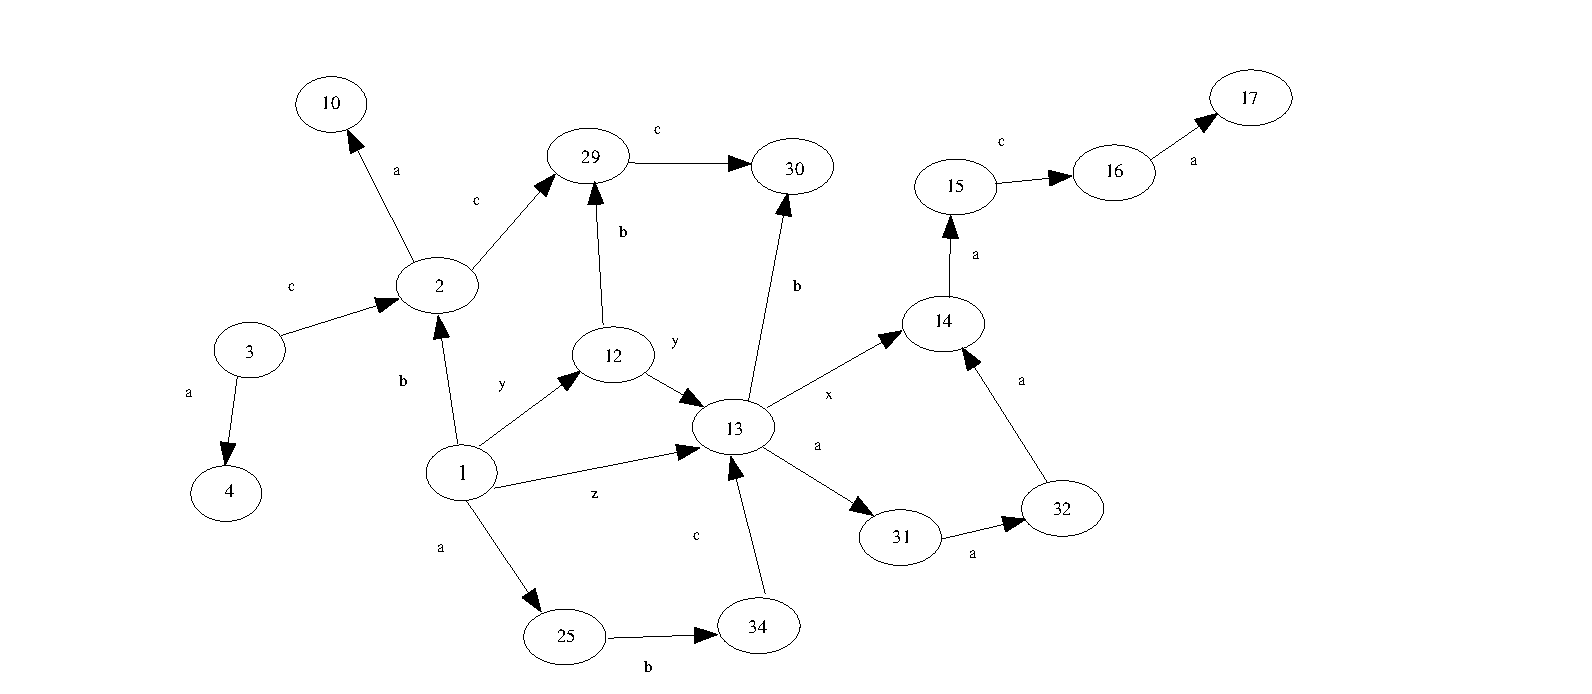
\includegraphics[scale=0.5, bb=0 0 680 480]{python/ex_K_f1.eps}
\caption{$X_1$ component $\Theta_1$}
\label{fig:K_f1}
\end{center}
\end{figure}

\begin{figure}
\begin{center}
\psfrag{a}{$x_1$}
\psfrag{b}{$x_2$}
\psfrag{c}{$x_3$}
\psfrag{r}{$y_1$}
\psfrag{s}{$y_2$}
\psfrag{t}{$y_3$}
\psfrag{x}{$z_1$}
\psfrag{y}{$z_2$}
\psfrag{z}{$z_3$}
\psfrag{u}{$y_4$}
\psfrag{1}{$1$}
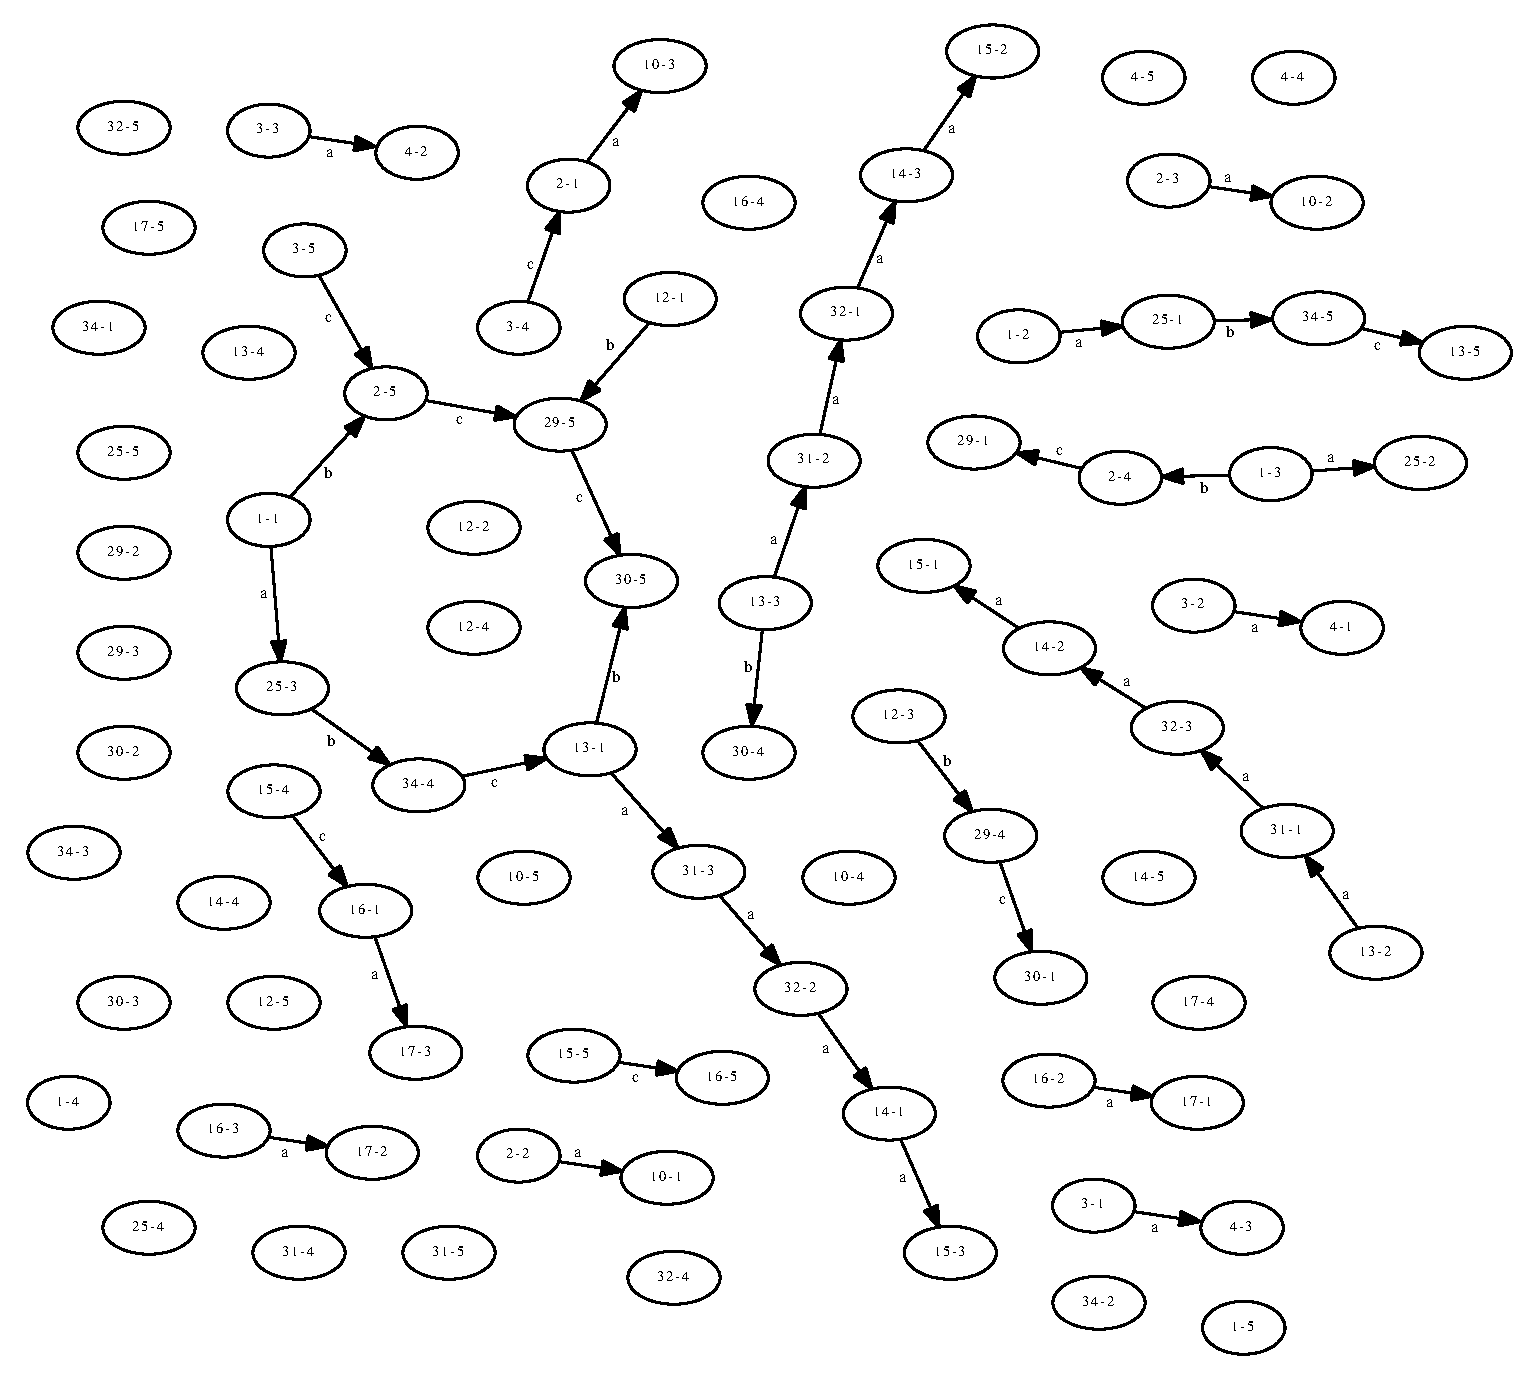
\includegraphics[scale=0.8, bb=0 0 500 480]{python/ex_K_f1-x-g.eps}
\caption{$\Theta_1\times \G_{A_1}$}
\label{fig:K_f1-x-g}
\end{center}
\end{figure}


\begin{figure}
\begin{center}
\psfrag{a}{$x_1$}
\psfrag{b}{$x_2$}
\psfrag{c}{$x_3$}
\psfrag{r}{$y_1$}
\psfrag{s}{$y_2$}
\psfrag{t}{$y_3$}
\psfrag{x}{$z_1$}
\psfrag{y}{$z_2$}
\psfrag{z}{$z_3$}
\psfrag{u}{$y_4$}
\psfrag{1}{$1$}
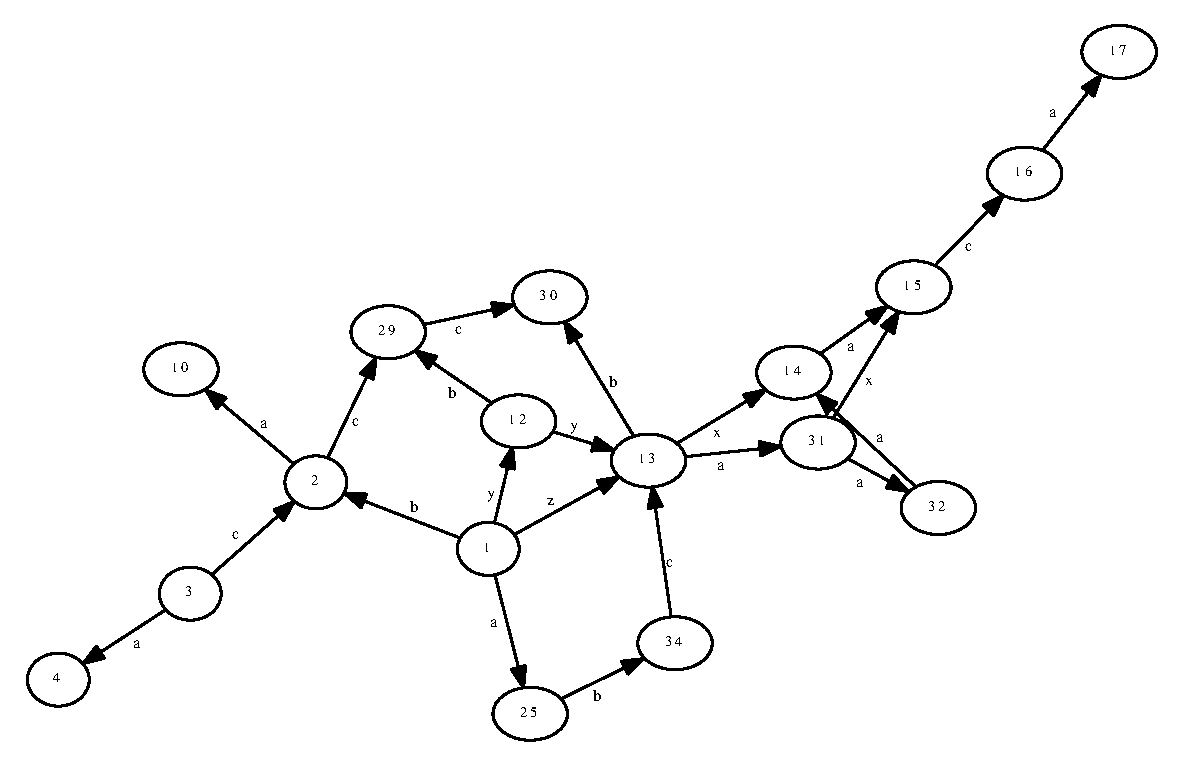
\includegraphics[scale=0.5, bb=50 200 580 580]{python/ex_K_f2.eps}
\caption{$X_1$ component $\Theta_2$}
\label{fig:K_f2}
\end{center}
\end{figure}

\begin{figure}
\begin{center}
\psfrag{a}{$x_1$}
\psfrag{b}{$x_2$}
\psfrag{c}{$x_3$}
\psfrag{r}{$y_1$}
\psfrag{s}{$y_2$}
\psfrag{t}{$y_3$}
\psfrag{x}{$z_1$}
\psfrag{y}{$z_2$}
\psfrag{z}{$z_3$}
\psfrag{u}{$y_4$}
\psfrag{1}{$1$}
\begin{subfigure}[b]{.3\columnwidth}
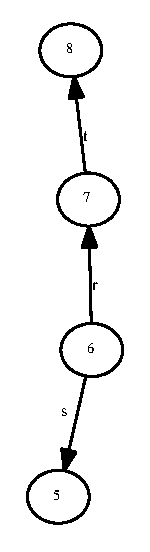
\includegraphics[scale=0.5, angle=90, bb=0 0  82 280]{python/ex_K_Y1.eps}
\caption{$\Theta^\prime$}
\label{fig:KY1}
\end{subfigure}
\hspace*{2cm}
\begin{subfigure}[b]{.3\columnwidth}
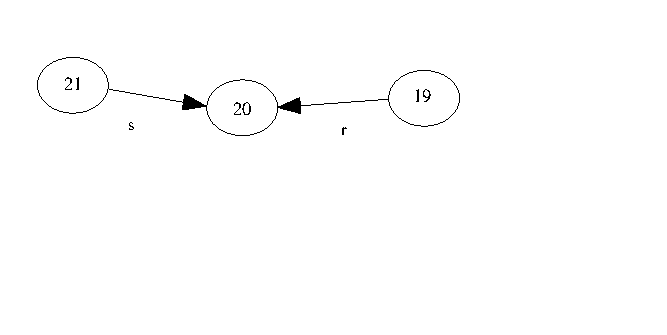
\includegraphics[scale=0.5, angle=90, bb=0 0 82 210]{python/ex_K_Y2.eps}
\caption{$\Theta^{\prime\prime}$}
\label{fig:KY2}
\end{subfigure}
\end{center}
\caption{$X_2$ components}
\label{fig:KY}
\end{figure}
\begin{figure}
\begin{center}
\psfrag{a}{$x_1$}
\psfrag{b}{$x_2$}
\psfrag{c}{$x_3$}
\psfrag{r}{$y_1$}
\psfrag{s}{$y_2$}
\psfrag{t}{$y_3$}
\psfrag{x}{$z_1$}
\psfrag{y}{$z_2$}
\psfrag{z}{$z_3$}
\psfrag{u}{$y_4$}
\psfrag{1}{$1$}
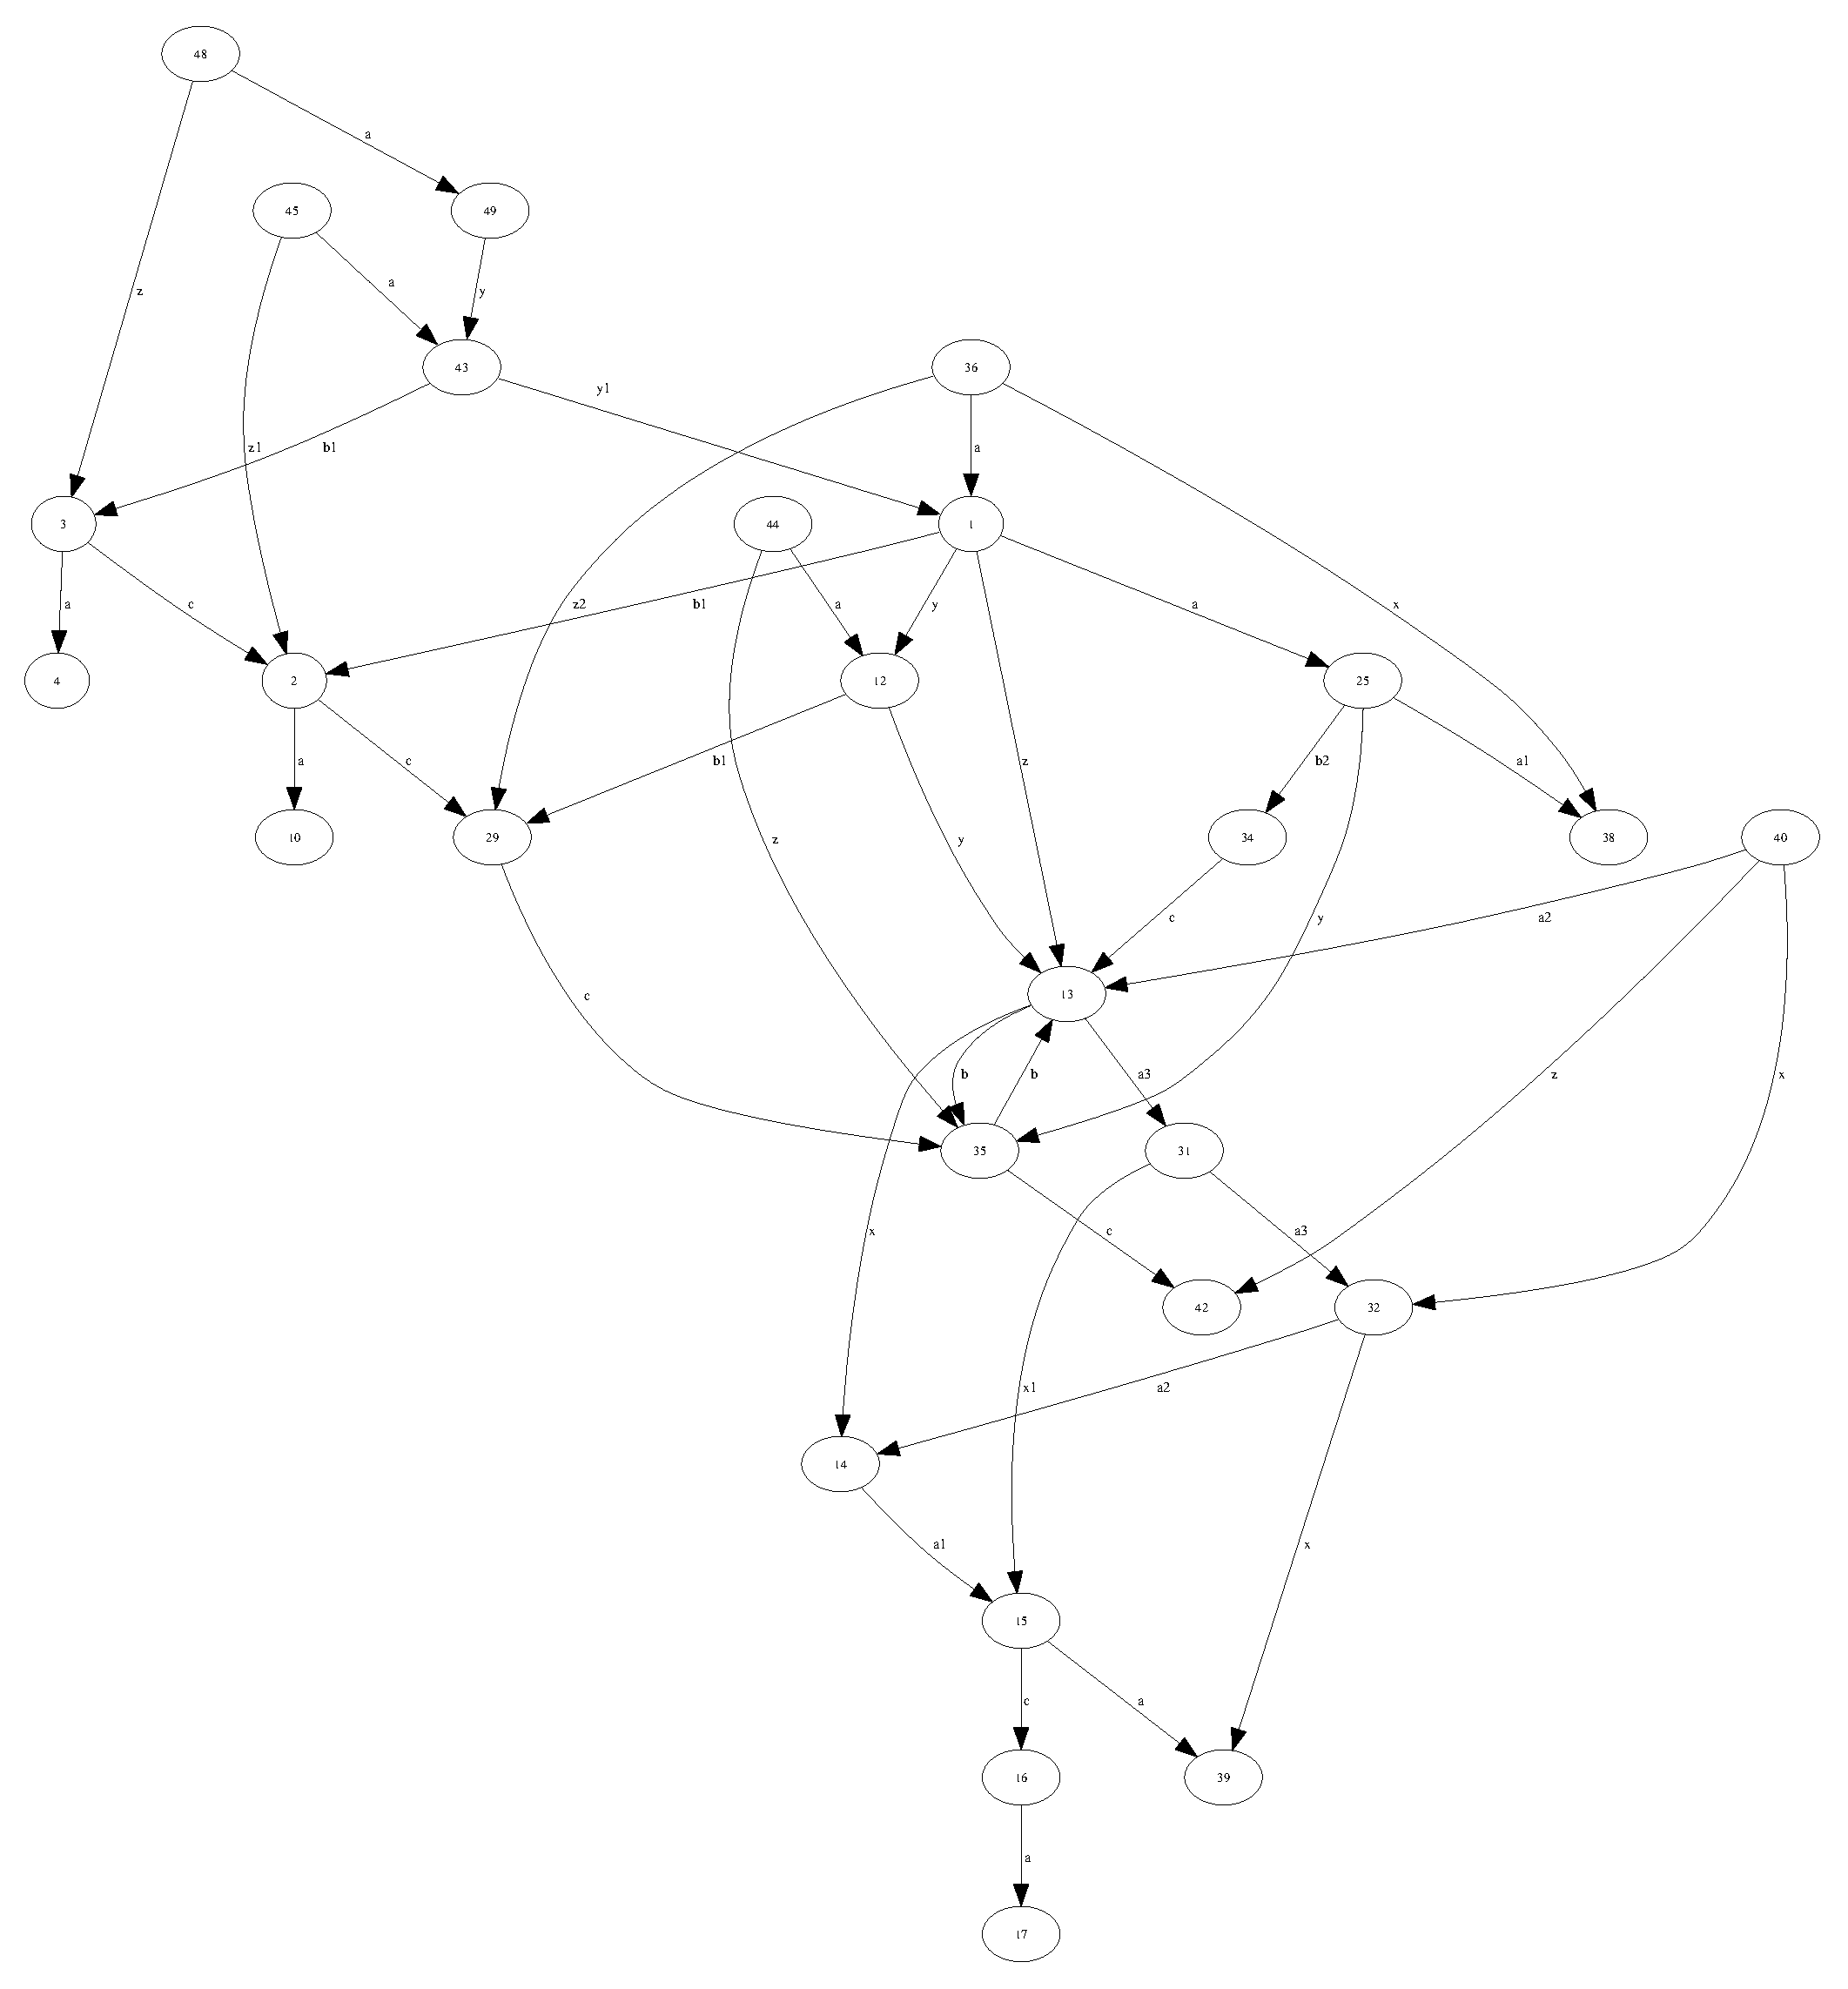
\includegraphics[scale=0.7,bb=0 0 820 720]{python/ex_K_f5.eps}
\caption{$\Theta_5$}
\label{fig:KX5}
\end{center}
\end{figure}
\begin{figure}
\begin{center}
\psfrag{a}{$x_1$}
\psfrag{b}{$x_2$}
\psfrag{c}{$x_3$}
\psfrag{r}{$y_1$}
\psfrag{s}{$y_2$}
\psfrag{t}{$y_3$}
\psfrag{x}{$z_1$}
\psfrag{y}{$z_2$}
\psfrag{z}{$z_3$}
\psfrag{u}{$y_4$}
\psfrag{1}{$1$}
\begin{subfigure}[b]{.3\columnwidth}
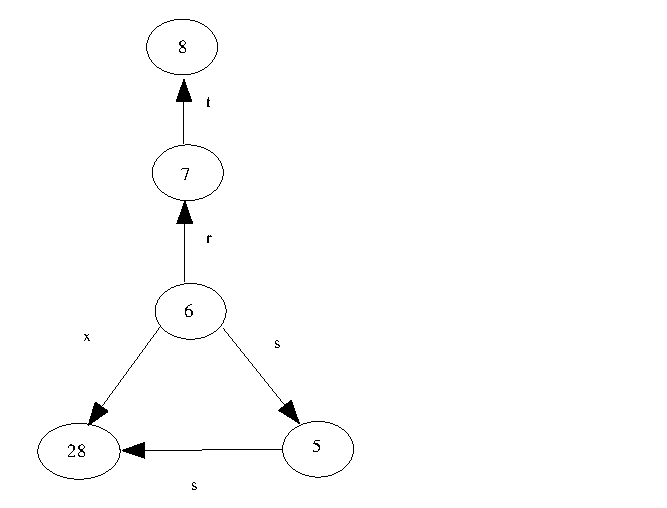
\includegraphics[scale=0.5, angle=90, bb=0 0  82 280]{python/ex_K_i4.eps}
\caption{$\Theta_5^\prime$}
\label{fig:KY15}
\end{subfigure}
\hspace*{2cm}
\begin{subfigure}[b]{.3\columnwidth}
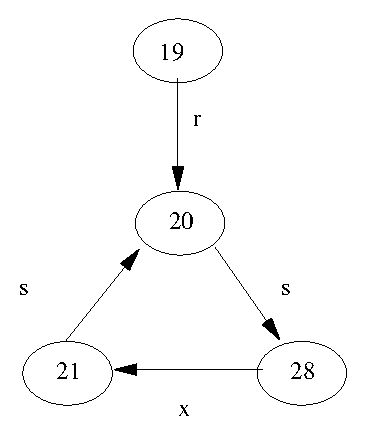
\includegraphics[scale=0.5, angle=90, bb=0 0 82 210]{python/ex_K_j4.eps}
\caption{$\Theta_5^{\prime\prime}$}
\label{fig:KY25}
\end{subfigure}
\end{center}
\caption{Modified $X_2$ components}
\label{fig:KY5}
\end{figure}
\begin{figure}
\begin{center}
\psfrag{a}{$x_1$}
\psfrag{b}{$x_2$}
\psfrag{c}{$x_3$}
\psfrag{r}{$y_1$}
\psfrag{s}{$y_2$}
\psfrag{t}{$y_3$}
\psfrag{x}{$z_1$}
\psfrag{y}{$z_2$}
\psfrag{z}{$z_3$}
\psfrag{u}{$y_4$}
\psfrag{1}{$1$}
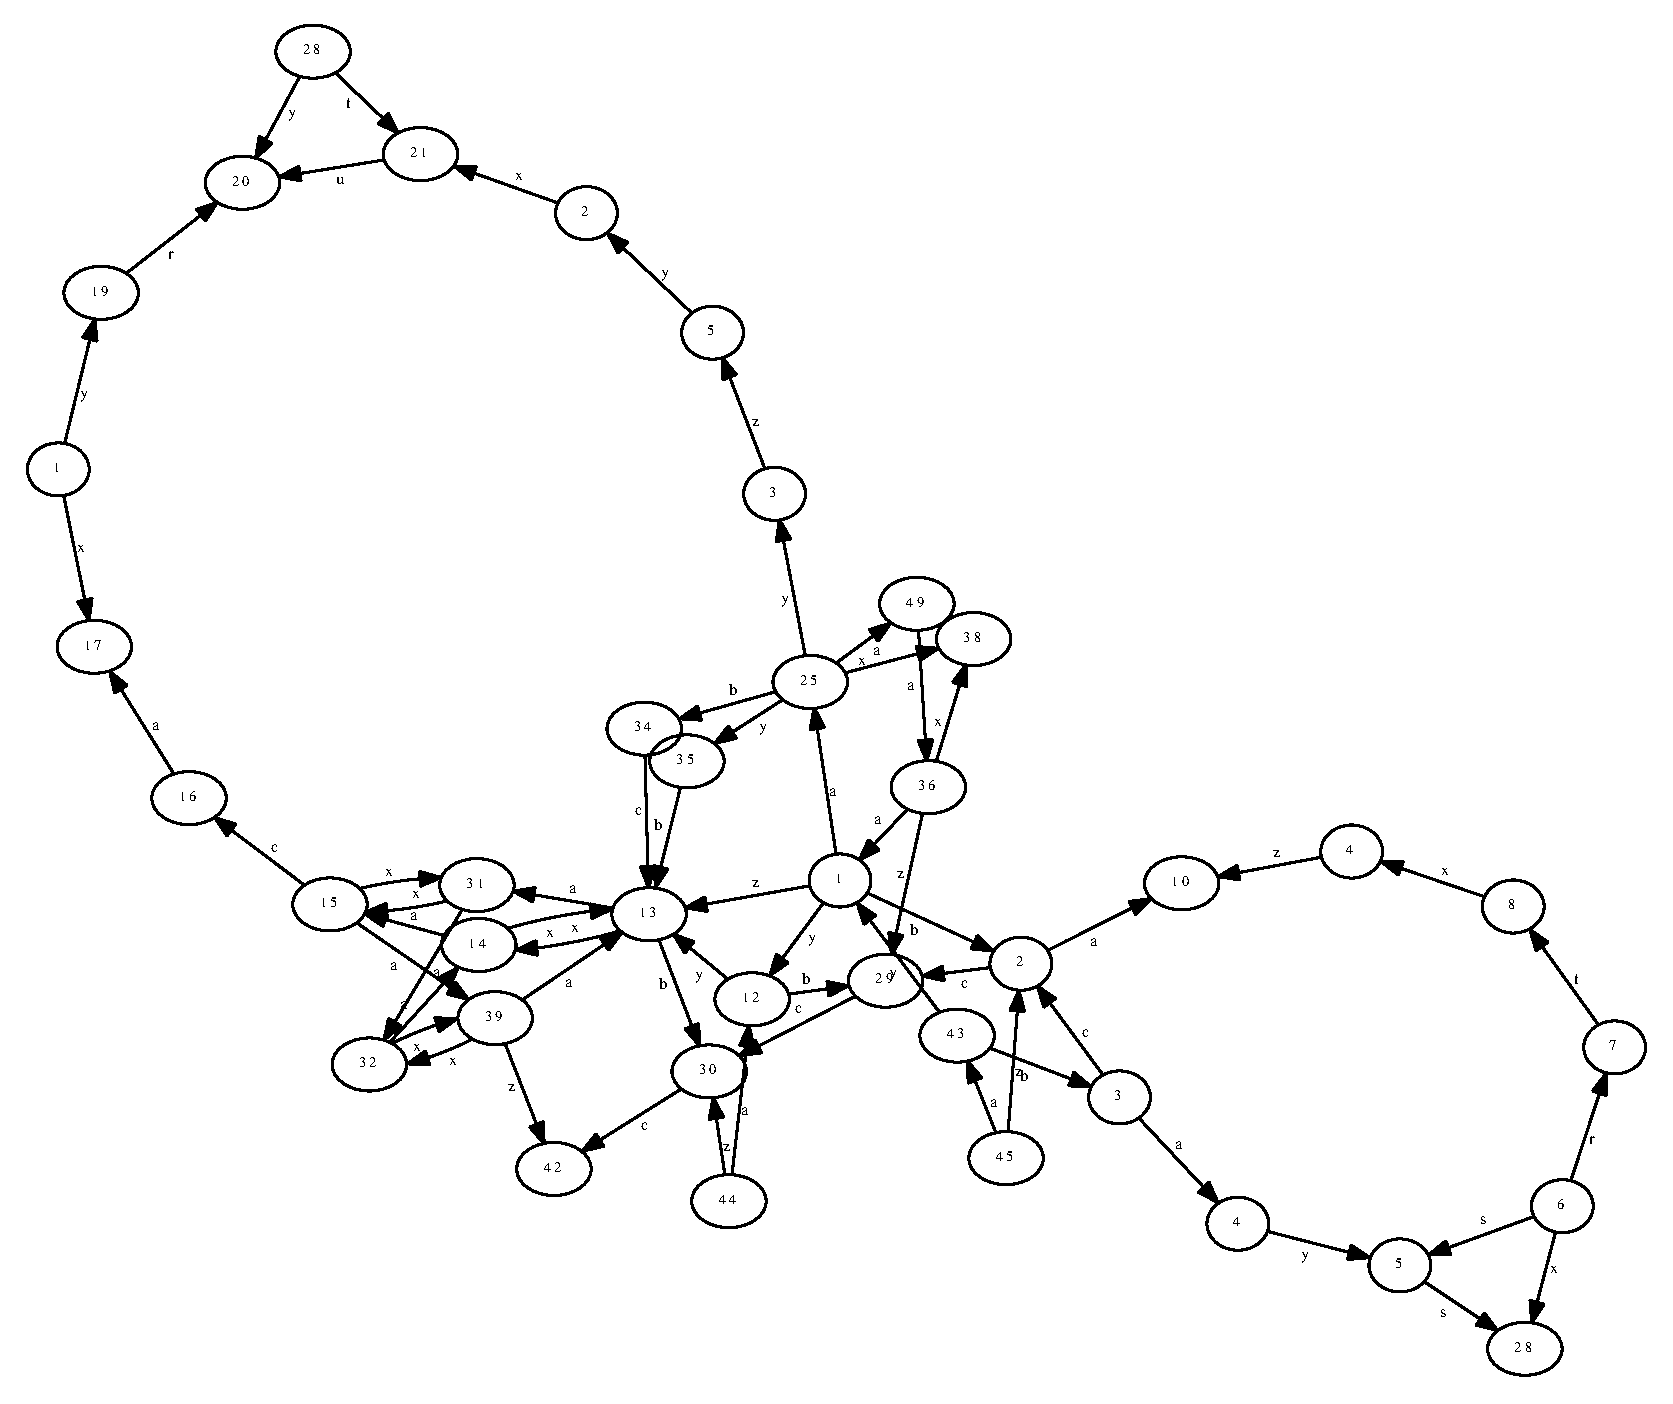
\includegraphics[scale=0.7,bb=0 0 820 720]{python/ex_K_reassembly.eps}
\caption{$\Psi$}
\label{fig:out}
\end{center}
\end{figure}
\begin{lemma}\label{lem:nfcomp}
Let $\a$ and $\b$ be boundary vertices of  an $X_k$ component $\T$ of
an inverse automaton $\D$, with alphabet $\S$. Then   the following hold.
\be
\item\label{it:nfcomp1}
  $\pi(L(\T,\a,\b))=\pi(L(\T_5,\theta(\a),\theta(\b)))$.
\item\label{it:nfcomp2} Let $w$ be a word
 which is accepted by the automaton $(\T, \a, \b)$. Then the
normal form of $w$ is accepted by $(\T_5, \theta(\a), \theta(\b))$.
\ee
\end{lemma}
\begin{proof}
\ref{it:nfcomp1}. 
At each stage of the modification process of Algorithm
II the image under $\pi$ of the language accepted by $(\T_i,\a,\b)$  was
preserved. 

\ref{it:nfcomp2}.
We may assume that $w\in \FF(X_k)$ (given the construction of $\T_1$).
Let $w$ have normal form $h_1s h_2^{-1}$, where $s\in S_k$ and $h_i\in \FF(Z)$.
There are two cases to consider, depending on whether $s$ is a
representative of type $1$ or type $2$.
 First consider the case where $s$ is of type $1$, say
 $s= a_1 e a_2^{-1}$, where
$a_1$ is a maximal $L_{Q_k}$-prefix and an $L_{T_k}$-prefix of $s$ and
 $a_2$  is a maximal $L_{Q_k}$-prefix and an $L_{T_k}$-prefix of $a_2\circ e^{-1}$.
 Then, as the normal form is the result of applying $\phi_k$ to the 
output of Algorithm I, 
 there are words
$g_1, g_2, b_1$ and $b_2\in \FF(X_k)$ such that
$w=g_1\circ b_1\circ e \circ b_2^{-1}\circ g_2^{-1}$,
$g_i\in H_k$, $b_1$ is a maximal $L_Q$-prefix of
$b_1\circ e \circ b_2^{-1}\circ g_2^{-1}$,
$b_2$ is a maximal $L_Q$-prefix of $b_2\circ e^{-1}$, $e\neq 1$,
$a_i=w(\t(b_i))$ and $\phi_k(h_i)=g_ib_ia_i^{-1}$, $i=1,2$.

Recall that we refer to the images of vertices of $\T$ in $\T_i$ as
 ``vertices of $\T$'', for $i=1,\ldots ,5$.
Since $g_i\in H_k$ and $w$ is accepted by $\T_1$ there is a path
labelled $g_1$ from $\a$ to a vertex $\a_1$ of $\T$ and a path
labelled $g_2$ from $\b$ to a vertex $\b_1$ of $\T$. Therefore, in $\cP$,
there are paths $p_1$ from $(\a,1)$ to $(\a_1,1)$ labelled $g_1$, and
$p_2$
from $(\b,1)$ to $(\b_1,1)$ labelled $g_2$.
(See Figure \ref{fig:nf-1}.)
\begin{figure}
\begin{center}
\psfrag{a}{$\a$}
\psfrag{b}{$\b$}
\psfrag{a1}{$\a_1$}
\psfrag{a2}{$\a_2$}
\psfrag{b1}{$\b_1$}
\psfrag{b2}{$\b_2$}
\psfrag{b_1}{$b_1$}
\psfrag{b_2}{$b_2$}
\psfrag{h1}{$h_1$}
\psfrag{c}{$e$}
\psfrag{w'1}{$w_1^\prime$}
\psfrag{w'2}{$w_2^\prime$}
\psfrag{s}{$s$}
\psfrag{h2}{$h_2$}
\psfrag{g1}{$\phi_k^{-1}(g_1)$}
\psfrag{g2}{$\phi_k^{-1}(g_2)$}
\psfrag{h'2a2}{$h_2^\prime a_2$}
\psfrag{h'1a1}{$h_1^\prime a_1$}
\psfrag{Th5}{$\T_4$}
\psfrag{cP}{$\cP_3$}
\psfrag{G_A}{$\G_{A_k}$}
\psfrag{(a,1)}{$(\a,1)$}
\psfrag{(a1,1)}{$(\a_1,1)$}
\psfrag{(a2,e1)}{$(\a_2,\e_1)$}
\psfrag{(b,1)}{$(\b,1)$}
\psfrag{(b1,1)}{$(\b_1,1)$}
\psfrag{(b2,e2)}{$(\b_2,\e_2)$}
\psfrag{g-1}{$g_1$}
\psfrag{g-2}{$g_2$}
\psfrag{b'_1}{$b_1^\prime$}
\psfrag{b'_2}{$b_2^\prime$}
\psfrag{a_1}{$a_1$}
\psfrag{a_2}{$a_2$}
\psfrag{e1}{$\e_1$}
\psfrag{e2}{$\e_2$}
\psfrag{r1}{$g_1$}
\psfrag{r2}{$g_2$}
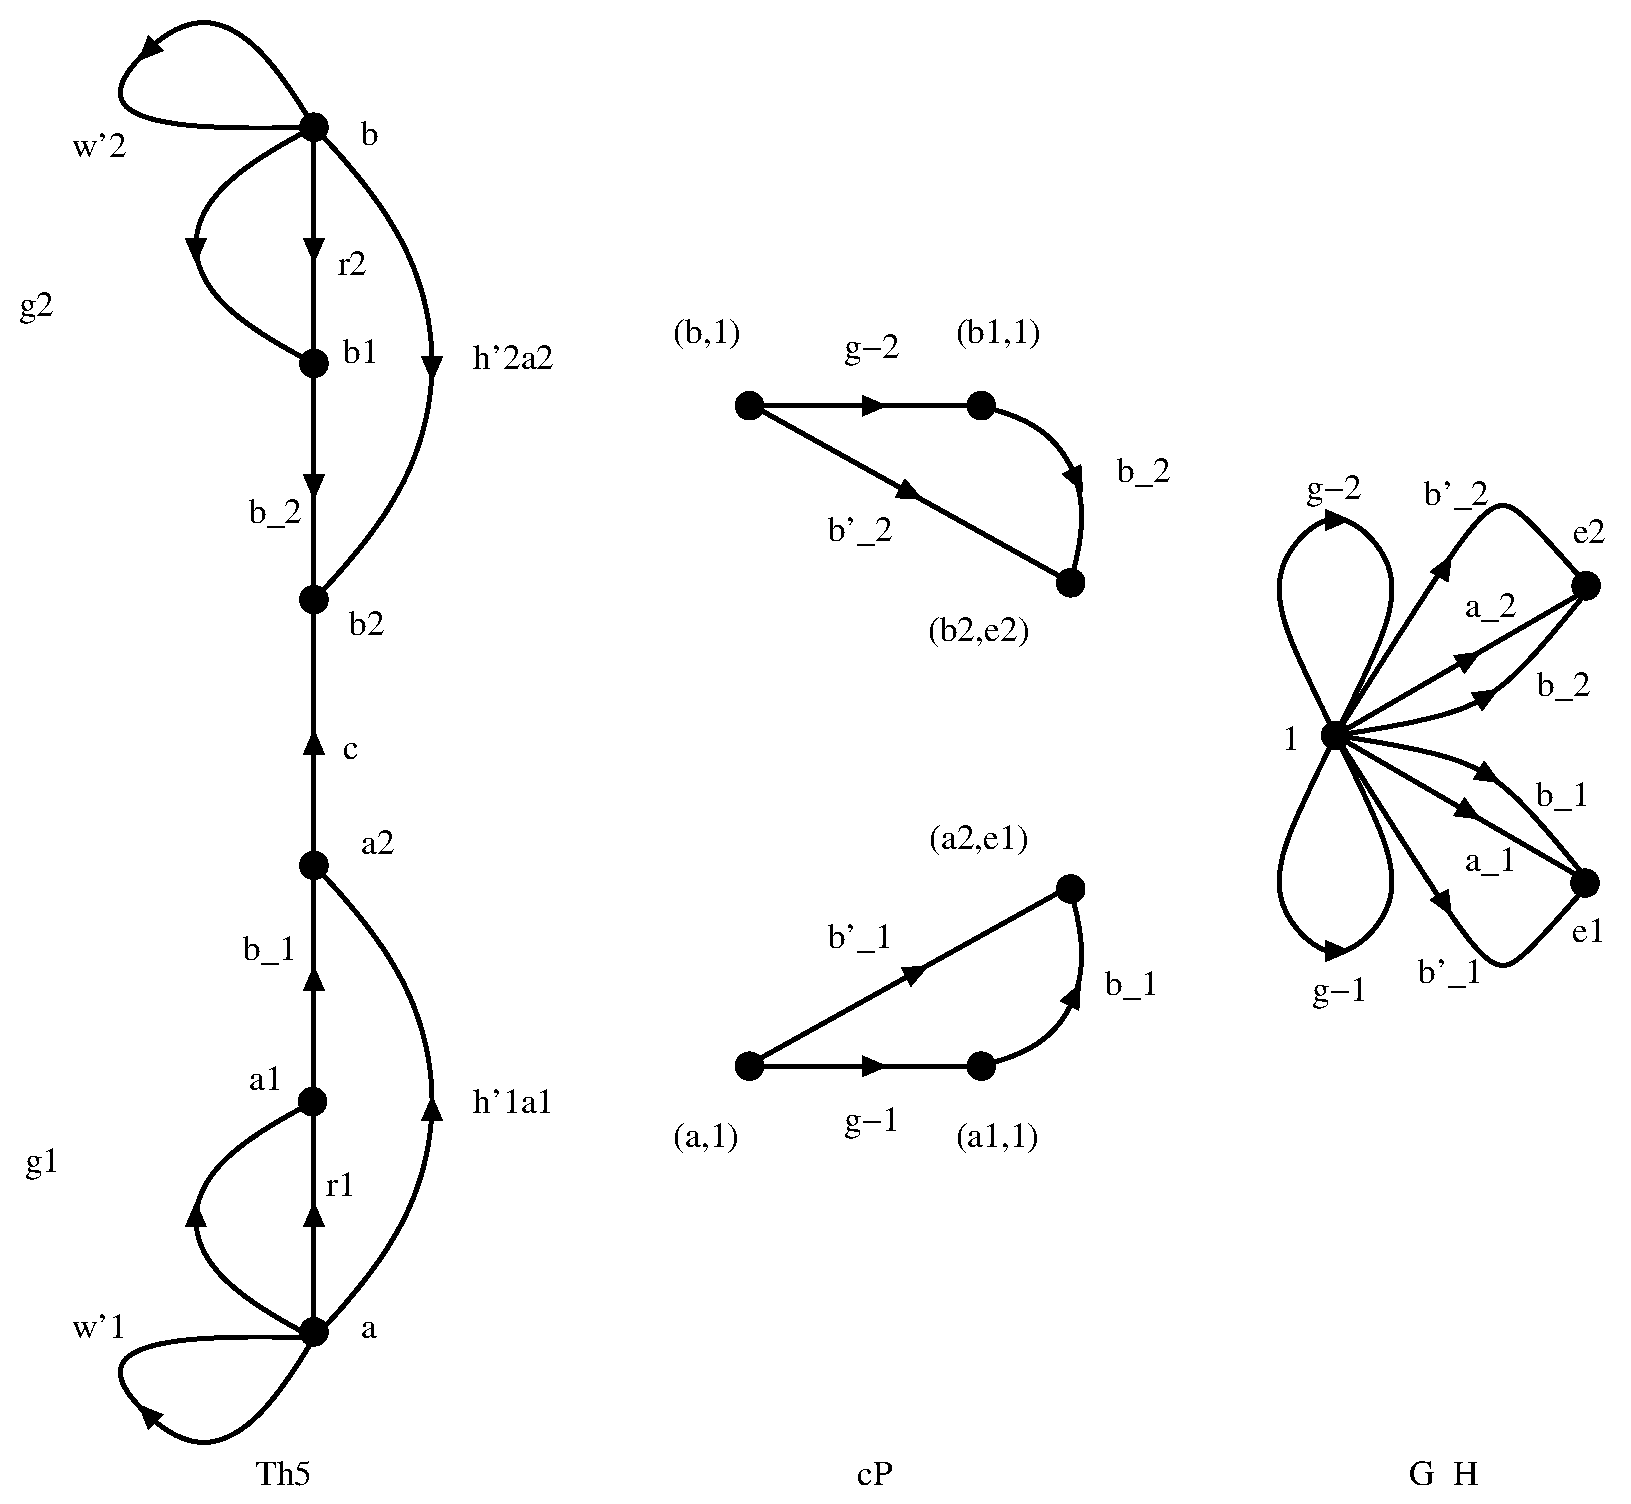
\includegraphics[scale=.5]{nf-1.eps}
\end{center}
\caption{Normal form: type 1.}
\label{fig:nf-1}
\end{figure}
Now $p_1$ may
be written as a concatenation of paths $p_1=o_0e_1\cdots e_l o_{l}$,
where $o_i$ is a simple path in $\U$ and $e_i$ is an edge of $\cP$ which does
not belong to $\U$.  Let $e_i$ have initial and terminal vertices
$\g_i$ and $\d_i$, and let $L_i$ and $R_i$ be the simple paths in $\U$ from
$(\a,1)$ to $\g_i$ and from $\d_i$ to $(\a,1)$, respectively.
In addition let $L_{l+1}$ be the path in $\U$ from $(\a,1)$ to
$(\a_1,1)$.
Then $L_1=o_0$ and, for $i=1,\ldots ,l$, $L_{i+1}=R_i^{-1}o_{i}$.
(See Figure \ref{fig:LeR}.)
\begin{figure}
\begin{center}
\psfrag{R1}{$R_1$}
\psfrag{L1}{$L_1$}
\psfrag{e1}{$e_1$}
\psfrag{o1}{$o_1$}
\psfrag{R2}{$R_2$}
\psfrag{L2}{$L_2$}
\psfrag{e2}{$e_2$}
\psfrag{o2}{$o_2$}
\psfrag{Rl}{$R_l$}
\psfrag{Ll}{$L_l$}
\psfrag{el}{$e_l$}
\psfrag{ol}{$o_l$}
\psfrag{o0}{$o_0$}
\psfrag{ol-}{$o_{l-1}$}
\psfrag{(a,1)}{$(\a,1)$}
\psfrag{(a1,1)}{$(\a_1,1)$}
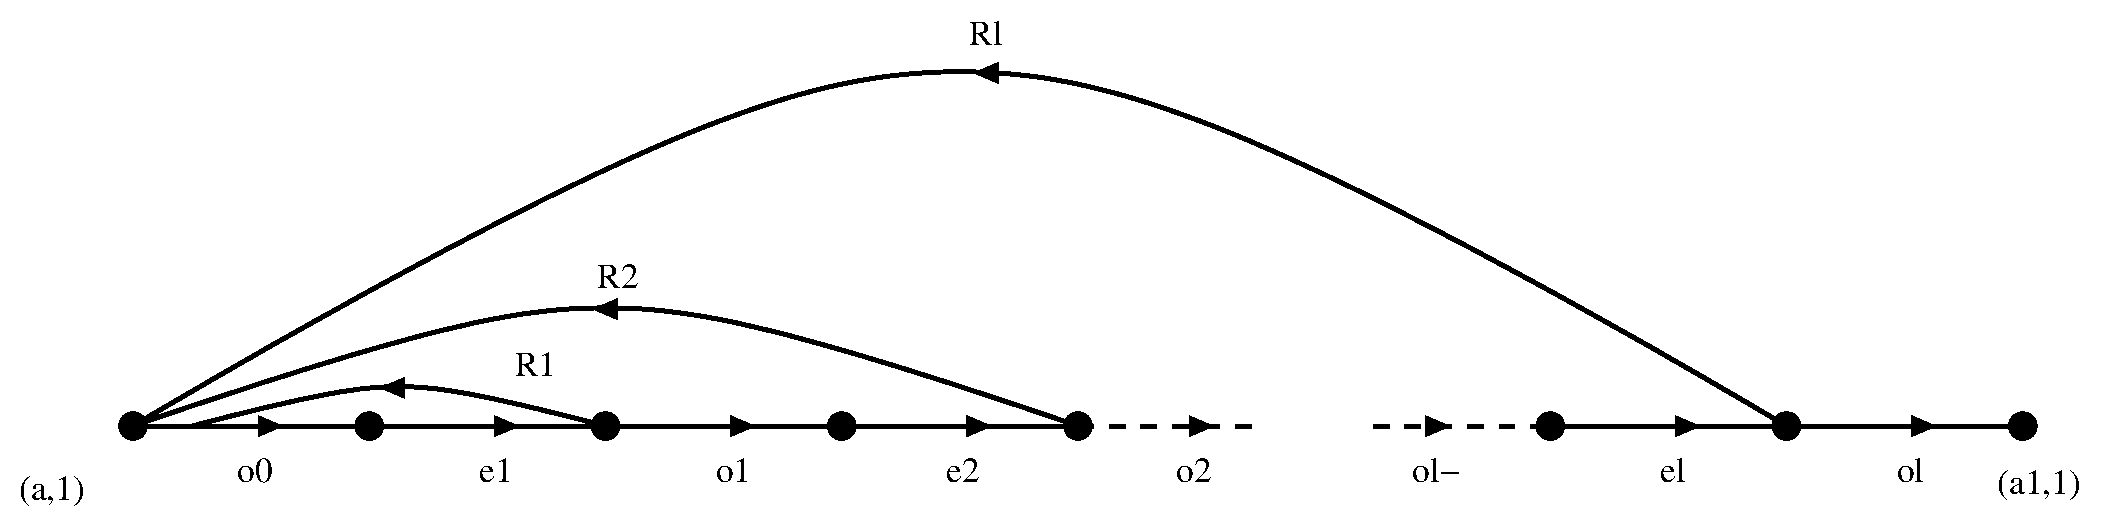
\includegraphics[scale=.4]{LeR.eps}
\end{center}
\caption{The path $p_1$.}
\label{fig:LeR}
\end{figure}
Moreover, for $i=1,\ldots ,l$,
the path $L_i e_i R_i$ is a closed path in $\cP$, based
at $(\a,1)$, containing exactly one edge, $e_i$, which is not in $\U$.
Thus the label of  $L_i e_i R_i$ is $v_i\in H_k$ and $\phi_k^{-1}(v_i)$ is the
label of a closed path in $\T_3$, based at  $\a$. (All such paths
were added in the construction of $\T_3$ from $\T_2$.)
Also, the path $L_{l+1}$, from $(\a,1)$ to $(\a_1,1)$, has
label $v_{l+1}\in H$,
and by construction of $\T_2$ there is a path from $\a$ to
$\a_1$ in $\T_2$ with label $\phi_k^{-1}(v_{l+1})$.
The path
$p_1$ is the result of reducing (deleting adjacent edges $e,e^{-1}$) the path
$o_0 e_1 (R_1 R_1^{-1}) o_1 \cdots e_{l}(R_l R_l^{-1}) o_{l}$, which
is equal to the path $L_1 e_1 R_1 \cdots L_l e_l R_l L_{l+1}$. Hence the label $g_1$
of $p_1$ is the result of
reducing the word $v_1\cdots v_l v_{l+1}$
 and $\phi_k^{-1}(g_1)$ is the result of
reducing $\phi_k^{-1}(v_1) \cdots \phi_k^{-1}(v_{l+1})$. As each $\phi_k^{-1}(v_i)$ is readable
in $\T_3$ and $\T_3$ is folded this means  that $\phi_k^{-1}(g_1)$ is the
label of a path, from $\a$ to   $\a_1$, in $\T_3$. Similarly,
$\phi_k^{-1}(g_2)$
is the label of a path from $\b$ to $\b_1$ in $\T_3$.

The word $b_1$ is readable by $\G_{A_k}$ and there
is a path with label $b_1$ in $\T_1$ from $\a_1$ to some vertex $\a_2$
of $\T$.
Hence $b_1$ is the label of a path in $\cP$ from $(\a_1,1)$ to
$(\a_2,\e_1)$, for some vertex $\e_1$ of $\G_{A_k}$.
By definition $a_1=w(\t(b_1))$ is the label of a path in $T_k$ from $1$ to $\e_1$.
Let $b_1^\prime$
 be the label of the simple path $p_1^\prime$ in $\U$ from
$(\a_1,1)$ to $(\a_2,\e_1)$ (see Figure \ref{fig:nf-1}). By construction $\T_4$ contains a path
from $\a_1$ to $\a_2$ with label $h_1^\prime a_1$, where
$h_1^\prime =\phi_k^{-1}(b_1^\prime a_1^{-1})\in \FF(Z)$.
(If $\cP$ covers the pair $(\a_1,1)$, $(\a_2,\e_1)$ then
$b_1^\prime=a_1$ and $h_1^\prime$ is the empty word, while there
exists a path with label $a_1$ from $\a_1$ to $\a_2$ in $\T_3$.)
%Furthermore we have
%$\pi(\phi_k(h_1^\prime)b_1^{\prime\prime})=\pi(b_1^\prime)$.
Now $b_1(b_1^\prime)^{-1}\in H_k$ and is the label of a closed
path  in $\cP$ based at $(\a_1,1)$; so by the
previous part of proof, $\T_3$ contains a closed path, based at $\a_1$,
 with label
$w_1^\prime=\phi_k^{-1}(b_1(b_1^\prime)^{-1})$. Hence, as it is folded,
$\T_4$ contains a path, from $\a$ to $\a_2$,
with label the reduced word obtained from the product
$\phi_k^{-1}(g_1)w_1^{\prime} h_1^\prime a_1$, that is
 $\phi_k^{-1}(g_1b_1a_1^{-1}) a_1=h_1a_1$.
 Similarly, $\T_1$ contains a path labelled $b_2$ from $\b_1$ to
some vertex $\b_2$ of $\T$, and $\T_4$ contains a path from
$\b$ to $\b_2$ with label $h_2a_2$.

As $w$ is the label of a path in $\T_1$ there is a path from $\a_2$ to
$\b_2$ in $\T_4$ with label $e$. Therefore, in this case, $\T_4$ contains
a path from $\a$ to $\b$ which has label the normal form of $w$.

In the second case,
let $w$ have normal form $h_1 a_1 a_2^{-1} h_2^{-1} $, where
$h_1$ and $h_2$ are in $\FF(Z)$,  $a_1$ and $a_2$ are labels
of simple paths in the subtree $T_k$ and $s=a_1a_2^{-1}$ is a double coset
representative of type $2$. Then there are words
$g_1, g_2, b_1, b_2, c$  in $\FF(X_k)$,  such that
$w=g_1\circ b_1 \circ b_2^{-1}\circ g_2^{-1}$,
$g_i\in H_k$, $b_1$ is a maximal $L_Q$-prefix of
$b_1 \circ b_2^{-1}\circ g_2^{-1}$, $b_2$ in
$L_Q$, $c=c(\t(b_1),\t(b_2))$ and $a_i=w(v_i)$, where
$(v_1,v_2)$ is the $\sim$ representative of $(\t(b_1),\t(b_2))$.



As in the first case there are paths in $\T_3$ labelled
$\phi_k^{-1}(g_1)$ and
$\phi_k^{-1}(g_2)$ from $\a$ to $\a_1$ and $\b$ to $\b_1$, respectively.
(See Figure \ref{fig:nf-2}.)
\begin{figure}
\begin{center}
\psfrag{a}{$\a$}
\psfrag{b}{$\b$}
\psfrag{a1}{$\a_1$}
\psfrag{a2}{$\a_2$}
\psfrag{b1}{$\b_1$}
\psfrag{b2}{$\b_2$}
\psfrag{g1}{$\phi_k^{-1}(g_1)$}
\psfrag{g2}{$\phi_k^{-1}(g_2)$}
\psfrag{Th5}{$\T_5$}
\psfrag{b_1}{$b_1$}
\psfrag{b_2}{$b_2$}
\psfrag{w}{$r$}
\psfrag{r1}{$g_1$}
\psfrag{r2}{$g_2$}
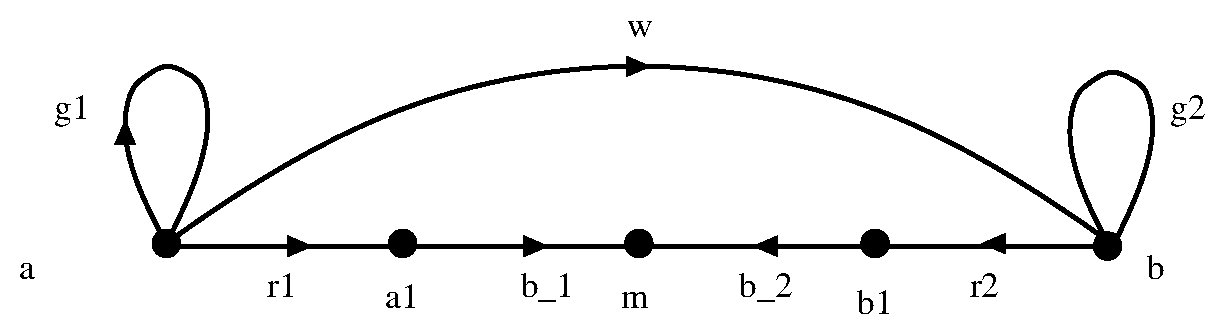
\includegraphics[scale=.5]{nf-2.eps}
\end{center}
\caption{Normal form: type 2, $r=\phi_k^{-1}(b_1ca_1^{-1})a_1a_2^{-1}\phi_k^{-1}(a_2c^{-1}b_2^{-1})$.}
\label{fig:nf-2}
\end{figure}
As $w$ is readable in $\T$ there is a path labelled $b_1b_2^{-1}$, from
$\a_1$ to $\b_1$, in $\T_3$.
By construction of $\T_5$ there is also a path labelled
$r=\phi_k^{-1}(b_1ca_1^{-1})a_1a_2^{-1}\phi_k^{-1}(a_2c^{-1}b_2^{-1})$
from $\a_1$ to $\b_1$. As $\T_5$ is folded
$
\phi_k^{-1}(g_1 b_1ca_1^{-1})a_1a_2^{-1}\phi_k^{-1}(a_2c^{-1}b_2^{-1}g_2)$
 is readable in
$\T_5$. Since the latter is in normal form we have
$h_1 = \phi_k^{-1}(g_1 b_1ca_1^{-1})$ and
$h_2= \phi_k^{-1}(g_2 b_2ca_2^{-1})$, as required.
\end{proof}

\begin{lemma}\label{lem:idverts}
Let $[\cdot]$ be the equivalence relation on $V(\D^\prime_5)$ above.
If $x$ and $y$ are vertices of $\D^\prime$, such that 
$[\theta(x)]=[\theta(y)]$ in $\D^{\prime\prime}$, then 
there exists a path in $\D$, from $\nu(x)$ to $\nu(y)$, with label $w$,
such that $\pi(w)=1$. 
\end{lemma}
\begin{proof}
Let $\a=\theta(x)$ and $\b=\theta(y)$. As $[\a]=[\b]$ there exists a
sequence of vertices $\g_0,\ldots ,\g_m$ of $\D^\prime_5$ such that 
$\a=\g_0$, $b=\g_m$ and 
\[\nu(\theta^{-1}(\g_i))\cap \nu(\theta^{-1}(\g_{i+1}))\neq \nul,\]
for $i=0,\ldots, m-1$. Suppose first that $m=0$. Then $\theta(x)=
\a=\b=\theta(y)$, so $x$ and $y$ both belong to some $X_k$ component
$\Theta$ of $\D^\prime$. As $\pi(L(\Theta,x,y))=\pi(L(\Theta_5, \a,\b)
=\pi(L(\Theta_5,\a,\a))$, there is a path in $\Theta$, from $x$ to $y$,
with label $w$, such that $\pi(w)=1$. $\Theta$ is embedded in $\D$ by the
map $\nu$, so the same holds for $\nu(x)$ and $\nu(y)$ in $\D$. 

Now assume that $m>0$ and that the result holds in all cases where the
sequence of $\g_i$'s above has length at most  $m$. Let 
$a\in  \nu(\theta^{-1}(\g_{m-1}))\cap \nu(\theta^{-1}(\g_{m}))$, and let 
$b,g$ be vertices of $\D^\prime$ such that $\nu(b)=\nu(g)=a$,   
$\theta(b)=g_m=\b$ and $\theta(g)=\g_{m-1}$. As $[\a]=[\g_1]=\cdots 
=[\g_{m-1}]=[\g_m]$, it follows from the inductive hypothesis that 
there is a path in $\D$, from $x$ to $a$, with label $w_1$, such
that $\pi(w_1)=1$. Moreover, $\theta(b)=\b=\theta(y)$, so it follows from
the case $m=0$, that there exists a path in $\D$, from $a$ to $y$,
with label $w_2$, such that $\pi(w_2)=1$. Concatenating these paths we
obtain the required result.
\end{proof}


\begin{lemma}\label{lem:dcfold}
Let $\D$ be  an inverse automaton, with alphabet $\S$ and start
state $s$, let $\D^{\prime\prime}$  and $\Psi$ be the
dc-resolution and dc-folding of $\D$, respectively, and 
let $\hat\rho:\D\maps \Psi$ be the dc-folding morphism. 
 
 Then the following hold. 
\be 
\item
\label{it:dcfold1} $\Psi$ is an inverse automaton, with unique
start and  final state $\s=\hat\rho(s)$, and has no more $X_1$ and
$X_2$ components than $\D$. 
\item \label{it:dcfold2}
$\pi(L(\Psi,\s))=\pi(L(\D,s))$. 
\ee
\end{lemma}
\begin{proof} ~
%\be
\ref{it:dcfold1}.
%\item
The automaton $\Psi$ is involutive and folded by definition.
 Its root is the image of the root $\rho(s)$ of $\D^{\prime\prime}$ under
 the folding morphism: that is $\hat\rho(s)$.
 As
$\D$ is connected  so is $\D^{\prime\prime}$ and therefore also
$\Psi$. Hence $\Psi$ is inverse. The graphs $\D$ and
$\D^{\prime\prime}$  have the same number of $X_k$ components.
Folding to form $\Psi$ cannot increase this number, so the final
statement of \ref{it:dcfold1} follows.
%\item
 \\[1em]
\ref{it:dcfold2}. Let $w$ be a word accepted by $\Psi=(\Psi,\s)$. Since
$\Psi$ is formed by a sequence of foldings of $\D^{\prime\prime}$,
there is a word $v$ such that $v$ is accepted by
$\D^{\prime\prime}$ (with root $\rho(s)$) and $\pi(v)=\pi(w)$. 
Thus $v$ is the label of a path $q_i$ in $\D^{\prime\prime}$, from  $\rho(s)$
to $\rho(s)$, and 
 $v=v_1\cdots v_n$,
where each factor $v_i$ is accepted by a connected component $\Xi_i$ of
$\D^\prime_5$;  and no two consecutive factors are accepted by the
same component. From Lemma \ref{lem:nfcomp}.\ref{it:nfcomp1} it
follows that there are paths $p_1,\ldots, p_n$, in $\D^\prime$,
with labels 
 $u_1,\ldots , u_n$, such that
$\pi(u_i)=\pi(v_i)$ and 
$p_i$ is a path in the component
$C_i=\theta^{-1}(\Xi_i)$ of $\D^\prime$.
Let the initial and terminal vertices of $p_i$ be $x_i$ and  $y_i$. 
As $\nu$ restricted to $C_i$ is an embedding, there is a path in $\D$,  from
$\nu(x_i)$ to $\nu(y_i)$ with label $u_i$, for $i=1,\ldots, n$.  

 Moreover, as $v$ is a path in $\D^{\prime\prime}$, based at $\rho(s)$, 
we have
\[[\theta(x_1)]=[\theta(y_n)]=\rho(s)\textrm{ and }[\theta(y_i)]=[\theta(x_{i+1})],\]
for $i=1,\ldots ,n-1$. From Lemma \ref{lem:idverts}, there exist paths in 
$\D$, 
\begin{itemize}
\item
from $s$ to $\nu(x_1)$, with label $w_0$;
\item  from $\nu(y_n)$ to $s$, with label $w_n$ and 
\item from $\nu(y_i)$ to $\nu(x_{i+1}$, with label $w_i$, for $i=1,\ldots,
n-1$,
\end{itemize}
such that $\pi(w_i)=1$, for $i=1,\ldots ,n$. Thus $l=w_0u_1\cdots w_{n-1}u_n
w_n$ is the label of a path in $\D$, based at $s$, such that
$\pi(l)=\pi(u_0\cdots u_n)=\pi(v)=\pi(w)$. 
 Therefore
$\pi(L(\Psi,\s))\subseteq \pi(L(\D,s))$. The reverse inclusion follows
from the existence of the morphism $\hat\rho$ from $\D$ to $\Psi$.
\begin{comment}
Let $\Phi=\L_0,\L_1,\ldots, \L_n$ be a sequence of graphs such that
$\L_{i+1}$ is obtained from $\L_i$ by and elementary folding.
Suppose that all these foldings except possibly the last involve only edges
of type $Z$. Assume $\L_n$ is formed from $\L_{n-1}$ by folding edges
$(\a,x,\b_1)$ and $(\a,x,\b_2)$ with label $x\in X_k$. Since the
first $n-1$ foldings involve only edges of type $Z$ it follows that
if $\g_1$ and $\g_2$ are vertices of $\Phi$ which map via these foldings
to $\b_1$ and $\b_2$, then there is a path $q$ in $\Phi$ from $\g_1$ to $\g_2$
which has label in $(Z^{\pm 1}\cup \{x^{\pm 1}\})^\ast$. Hence $\g_1$ and $\g_2$ both belong to
 the same $X_k$ component of $\Phi$, which also contains the path $q$.
Therefore all $n$ foldings can be carried out in this $X_k$
component. However the $X_k$ components of $\Phi$ are folded, since they
correspond to the graphs $\T_5$ constructed from $X_k$ components of $\D$.
Therefore no folding involving an edge of type $X_1$ or $X_2$ can occur
in such a sequence, and the result follows.
\end{comment}
%\ee
\end{proof}
If $w$ is a word in $\FF(X_1\cup X_2\cup Z)$ and $w=w_1\cdots w_n$,
where $w_i\in \FF(X_{k_i}\cup Z)$, with $k_i\neq k_{i+1}$ and $n$
minimal, then  say that each $w_i$ is a \emph {maximal} $X_{k_i}$
\emph{factor}
of $w$.
\begin{lemma}\label{lem:loopstop}
Let $\D_0$ be an inverse automaton with alphabet $\S$.
\be
\item\label{it:loopstop1}
If $\D_0$ is input  to  the loop then the loop halts after
finitely many iterations and outputs an inverse automaton  $\D_n$.
\item\label{it:loopstop2} Let $\D_n$ be the output from the loop and let $w$ be a word
accepted by $\D_0$. If $w=a\circ b \circ c$,
where $b$ is a maximal $X_k$ factor of $w$ then $\D_n$ accepts
the word $avc$, where $v$ is the normal form of $b$.
\ee
\end{lemma}
\begin{proof}
\ref{it:loopstop1}. The number of $X_k$ components is not
increased by Steps 1 and 2, so at some point the loop must halt.
\noindent \ref{it:loopstop2}. The word $b$ is accepted by an $X_k$
component of $\D_0$. By construction, the word $v$ is accepted by
$\D_1$, and hence by $\D_n$. It follows that $\D_n$ accepts $avc$.
\end{proof}
\begin{lemma}\label{lem:nfacc}
Let $\D_0$ be an inverse automaton with alphabet $\S$ and let
$\D_n$ be the output from the loop, with input $\D_0$. If $w$ is
accepted by $\D_0$ then the normal form of $w$ is accepted by $\D_n$.
\end{lemma}
\begin{proof}
Let $w$ be a word accepted by $\D_0$. Then $w$ factorises as  $w$
as $w=w_1\cdots w_n$, where $w_i$ is accepted by an $X_k$
component of $\D_0$. Thus $w_i\in \FF(X_{k_i}\cup Z)$, with $k_i\neq
k_{i+1}$. If $n=0$, then $w=1$ and the lemma holds. Suppose the
lemma holds for all $w$ such that $n\le k$, where $k\ge 0$ and now
suppose $n=k+1$. Let $v_i$ be the normal form of $w_i$. If $v_i\in
\FF(Z)$, for some $i$ then there is a factorisation of $w$ with at
most $k$ factors, and the result follows. Otherwise, from Lemma
\ref{lem:loopstop}.\ref{it:loopstop2},  $\D_n$ accepts $v_1\cdots
v_n$, which is the normal form of $w$.
\begin{comment}
Let $\g$ and $\d$ be vertices of $\Phi$ which map to $\a$ and $\b$ in the
folding of $\Phi$ to $\L$. As this folding involves only edges of type $Z$
it follows that $\g$ and $\d$ are in the same $X_k$ component of $\Phi$.
Moreover there is a path $p^\prime$ in $\Phi$ such that the image
of $p^\prime$ in $\L$ reduces to $p$. Then $\Phi$ contains a path
$q^\prime$ such that the label of $q^\prime$ is the normal form of
the label of $p^\prime$. Let $q$ be the reduced path in $\L$ obtained by
reduction of the image of $q^\prime$. Then the images of $l(q)$ and
$l(q^\prime)$ in $G$ are equal and both are equal to the image of $l(p)$ in
$G$. Moreover, since $l(q^\prime)$ is in normal form and $l(q)$ is obtained
from $l(q^\prime)$ by cancellation of letters of $Z$ it follows that
$l(q)$ is in normal form. Hence $l(q)$ is the normal form of $l(p)$,
as required.
\end{comment}
\end{proof}
\begin{comment}
\begin{theorem}
Let $\cA=(\L,\S)$, where $\L$ is defined in the previous
lemma and $\ast$ is the root of $\L$. Then $\pi(L(\cA))=K$ and if $w$ is the normal form of an element
of $K$ then $w\in L(\cA)$.
\end{theorem}
\begin{proof}
We have $\pi(L(\cA))=\pi(L(\cF(K))=K$, by construction. If $u$ is a word
accepted by $\cA$ then we may write $u=z_0t_1z_1\cdots z_rt_rz_{r+1}$, where
$z_i\in \FF(Z)$ and $t_i$ is the label of a path between two boundary
vertices of an $X_1$ or $X_2$ component of $\L$, for all $i$. If
$s_i$ is the normal form of $t_i$ then, from the previous lemma, it follows
that $\cA$ also accepts the word $z_0s_1z_1\cdots z_rs_rz_{r+1}$, which
is the normal form of $u$.
\end{proof}
\end{comment}
\begin{theorem}
$G$ has solvable membership problem.
\end{theorem}
\begin{proof}
Construct the flower automaton $\cF(K)$ of $K$ and then
its Stallings automaton $\G_K$,  as at the beginning of this Section. % \ref{sec:dca},
Let $\D_0=\G_K$ and input this to the loop to obtain output $\D_n$.
Given a word $w\in \FF(X_1\cup X_2\cup Z)$ write $w$ in normal form
using Algorithm I. If $w\in K$ then there is a word $v$ in the generators
 of $K$ with $\pi(v)=\pi(w)$, so $v$ is accepted by $\G_K$. From
Lemma \ref{lem:nfacc}, the word $w$ is accepted by $\D_n$. From
Lemma \ref{lem:dcfold}.\ref{it:dcfold2}, $L(\D_n)=L(\G_K)$,
so if $w\notin K$, then
$w\notin L(\D_n)$.
\end{proof}

\section{The computational complexity}\label{sec:TC}

{\ef{Some words on time complexity needed!}}


Let $H$ be a finitely generated subgroup of $F=\FF(X)$ and
$Y=\{h_1,\ldots ,h_m\}$ be a generating set for $H$, where $h_i\in
F$. Consider the Stallings automaton $\G = \G_Y(H)$ for $H$ with
vertices $V\G$, edge set $E\G$ and the root vertex $1$. Denote by
$N$ the total length of $Y$, i.e. $N = |h_1| + |h_2| + \ldots +
|h_m|$. Notice that by construction of $\G$ we have $|V\G| \le N,
|E\G| \le N$, and $|E \G| \ge |V \G|$.

Given a set of generators $Y$ for $H$, one can construct the
Stallings automaton $\G$ for $H$ in time at most $t_1(N)$, where
\begin{equation}\label{t1} t_1(n) = O (n \cdot log^{\ast}(n)),
\end{equation}
where the function $log^{\ast}: \NN \rightarrow \NN$ is such that
$log^{\ast}(2n) = log^{\ast}(n) + 1$ (we are using the base $2$
logarithm), see \cite{touikan} for more details. For most
practical purposes, $log^{\ast}$ can be considered a constant
since it grows very slowly.

Further, below we will use frequently the time complexity of a
spanning subtree construction and complexity of taking graph
products.

Observe, that one can find a spanning subtree of a graph $\G$ in
time at most $t_2(|E\G|)$ or $t^{\prime}_2(|V\G|)$, where
\begin{equation}\label{t2}
t_2(n) = O(n \cdot log(n)) {\textrm{ and }} t^{\prime}_2(n) =
O(n^2),
\end{equation}

with a help of Kruskal's ($\G$ is arbitrary, and if it is not
connected, then it founds spanning subforest of $\G$) or
Jarnik-Prim's (the graph $\G$ supposed to be connected) algorithm,
respectively.

Computation of $\G_1 \times \G_2$ takes time at most $t_3(|V\G_1|,
|V\G_2|)$

\begin{equation}\label{t3}
t_3(n_1, n_2) = O(n_1 \cdot n_2).
\end{equation}

We will use notations of complexity functions $t_1, t_2, t'_2$,
and $t_3$ in what follows.

We write $O(f(n_1)) \preceq O(f(n_2))$ if $n_1\le n_2$ and $f$ is
a nondecreasing function. Observe that if $O(f(n_1)) \preceq
O(f(n_2))$ and an algorithm solve the problem in time $O(f(n_1)$,
then it all the more solve this problem in time $O(f(n_2))$.

\subsection{The time complexity of double coset normal forms construction}\label{sub:doubleCo_nf}

Recall that $F_1$, $F_2$ are free groups, and subgroups $H_1 \leq
F_1$, $H_2 \leq F_2$ have finite bases $Y_1 = \{h_1, \ldots, h_m
\}$ and $Y_2=\{h_1', \ldots, h_m'\}$, respectively, and there are
maps $\phi_k$ such that $\phi_1(z_i)=h_i$ and
$\phi_2(z_i)=h^\prime_i$, $i=1,\ldots ,m$, where $Z=\{z_1, \ldots,
z_m\}$, $\FF(Z)$ is a free group and $H_1$ isomorphic to $H_2$ via
$\phi_2 \phi_1^{-1}$, and ${G = F_1 \underset{H_1=H_2}{\ast}
F_2}$. To distinguish the length of elements in alphabets $X_k$ or
$Z$, we write $|\cdot|_k$ or $|\cdot|_Z$, correspondingly. Set
$N_1 = |h_1|_1 + |h_2|_1 + \ldots + |h_m|_1$ and $N_2 = |h_1|_2 +
|h_2|_2 + \ldots + |h_m|_2$. Let $A_k$ be the Stallings automaton
for $H_k$ and let $T_k$ be a spanning tree for the associated
graph $\G_{A_k}$, as above. Define $E\G_{A_k}$ to be an edge set
of $\G_{A_k}$, and let $V\G_{A_k}$ be its vertex set; let $N_k$ be
the total length of $Y_k$ ; definitions of $L_{Q_k}$ and $L_{T_k}$
were given in \ref{sub:foldings}, $k=1,2$. Let $S_k$ be the set of
double coset representatives of $H_k\le F_k$, defined by $T_k$.
The following lemma estimates the complexity of $S_k$
construction.

\begin{lemma}\label{lem:dctransversal} Let $w \in F_k \smallsetminus H_k$. Given a finite basis $Y_k$ of $H_k$, one can rewrite $w$ in a double coset normal
 form in time at most $O(N_k^2 + |w|_k)$.
\end{lemma}

%we can't formulate another lemma about time necessary for $S_k$ construction because we actually do not construct $S^{(1)}_k$ at all.

\begin{proof}
To rewrite an element $w$ in a double coset normal form, it is
sufficient to compute $\G_{A_k}$, sets $\L_{T_k}$, $L_{Q_k}$ (or
its subset $L^{\prime}_{Q_k}$, as we are doing below), and
$S^{(2)}_k$. Given these structures, one can easily rewrite $w \in
F_k$ in normal form, using Algorithm I.

Construction of $\G_{A_k}$ takes at most $t_1(N_k)$ steps, whereas
computation of its square
 $\G_{A_k} \times \G_{A_k}$ can be proceeded in at most
 $t_3(|V\G_{A_k}|,|V\G_{A_k}|) \preceq t_3(N_k,N_k)$.
A spanning subtree $T_k$ can be found in
$t^{\prime}_2(|V\G_{A_k}|) \preceq t^{\prime}_2(N_k)$ or $t_2(|E
T_k|) \preceq t_2(E\G_{A_k}) \preceq t_2(N_k)$; here the best
estimate in terms of $N_k$ is $O(N_k^2)$. Further, the time
required for $L_{T_k}$ computation is linear on $|E T_k|$, while
$L^{\prime}_{Q_k}$ can be computed in time linear on
$|V\G_{A_k}|$, where $L^{\prime}_{Q_k} \subset L_{Q_k}$ is a
subset of words in $L_{Q_k}$ which have no nontrivial prefixes
accepted by $\G_{A_k}$. To construct the set $P_0$ of $\sim$
representatives (see definition \ref{def:repres_t2}), one should
analyze all vertex sets of connected components of $\G_{A_k}
\times \G_{A_k}$, and the required time for this procedure is at
most $O(V \G_{A_k} \times \G_{A_k}) \preceq O(N^2_k)$, which
coincide with a maximal time required for construction of double
coset representatives of type $2$ (i.e. $S^{(2)}_k$).

Given $\G_{A_k}$, $L_{T_k}$, $L^{\prime}_{Q_k}$ and $S^{(2)}_k$
(observe that we spent at most $O(N^2_k)$ time on their
construction), we apply Algorithm I to $w \in F_k$. The analysis
of Algorithm I show that it take at most $O(|w|_k)$ time to obtain
a double coset normal form of $w$. Gathering both estimates
together, obtain $O(N^2_k + |w|_k)$, as required.
\end{proof}

\begin{corollary}\label{cor:dcnf_time} Suppose $g \in G$ and $g=g_1 \cdots g_t$ is in reduced
form. Given $Y_1, Y_2$, one can rewrite $g$ in double coset normal
form in time at most $O(N^2_1+ N^2_2 + |g_1|_{\e_1}+|g_2|_{\e_2}+
\ldots +|g_t|_{\e_t})$, where $\e_i \in \{ 1, 2\}, i = 1, \ldots,
t$, and $\e_i = k$ if $g_i \in F_k$.
\end{corollary}

\begin{proof} Notice first, that if $g = g_1 \in H_k$, then we
only rewrite it in terms of alphabet $Z$ which takes time at most
$O(|g_1|_k)$, and the case $g \in F_k \smallsetminus H_k$ is
covered by lemma \ref{lem:dctransversal}, so suppose $g \notin
F_k$, $k=1,2$.

One can rewrite each syllable $g_i \in F_k$ of $g$ in normal form
$g_i=h_{i,1}d_ih_{i,2}$, where $d_i\in S$ and $h_{i,j}\in H_1\cup
H_2$, in time at most $O(N^2_k + |g_i|_k)$. Using $\phi_1^{-1}$ or
$\phi_2^{-1}$, we write $h_{i,1}$ and $h_{i,2}$ as reduced words
in $\FF(Z)$ (for $i=1, \ldots, t$) and find the reduced word
$h_{i,2}h_{(i+1),1}\in \FF(Z)$ (for $i=1, \ldots, t-1$) in time at
most $O(|g_i|_{\e_i}+|g_i|_{\e_{i+1}})$, so the resulting
complexity of the process is at most $O(N^2_1+ N^2_2 +
|g_1|_{\e_1}+|g_2|_{\e_2}+ \ldots +|g_t|_{\e_t})$. \end{proof}


\subsection{The complexity of Algorithm II}\label{sub:resolution}

Let $K=\la k_1, \ldots , k_s\ra$, where $k_i$ is an element of $G$
written in normal form (\ref{eq:k-form}): $k_i=
h_{i,0}t_{i,1}h_{i,1}\cdots t_{i,m_i}h_{i,m_i+1}$, with
$h_{i,j}\in \FF(Z)$ and $t_{i,j}\in S_1\cup S_2$ as in section
\ref{sec:dca}. Recall that $\G$ is the rooted graph, associated to
a flower automaton $\cF(K)$ of the subgroup $\hat K < \FF(X_1\cup
X_2 \cup Z)$ generated by $k_1, \ldots , k_s$.

Consider the Stallings folding $\G_K$ of $\G$. Clearly, one can
construct $\G_K$ in time at most $t_1(M)$, with $M = M_Z+M_1+M_2$,
 $M_Z =
\mathop{\sum}\limits_{i=1}^{s}
\mathop{\sum}\limits_{j=1}^{m_i}|h_{i,j}|_Z$, and $M_k$ is the
total length of $t_{i,j} \in S_k$ in terms of $X_k$ for all
appropriate $i,j$, i.e. $M_k = \mathop{\sum}\limits_{i,j:
t_{i,j}\in S_k} |t_{i,j}|_k$, and the function $t_1$ defined by
(\ref{t1}); $k=1,2$.

Let $\D=\D_{(0)} = \G_K$ and let $\T^{(1)}, \ldots, \T^{(p_1)}$ be
the set of all $X_1$ components of $\D$, $\Phi^{(1)}, \ldots,
\Phi^{(p_2)}$ be the set of all $X_2$ components.

We shall study first the complexity of modifications $1-5$ for an
arbitrary $X_k$ component $\T$ of $\D$, and then apply this result
to estimate the general complexity of the Algorithm II. Denote by
$E_k \T$ the set of edges of type $X_k$ in $\T$, and let $E_Z \T$
be the set of edges of type $Z$ in $\T$, while $V \T$ denote its
vertex set.


\begin{lemma}\label{lem:resolution} Suppose $\D = \G_K$, $\G_{A_k}$, $T_k$ and $S^{(2)}_k$ are given and
$\T$ is an $X_k$ component of $\D$. Then one can modify $\T$ into
$\T_5$ in time at most $O(|V \G_{A_k}|^6 \cdot
|V\T|^{10}+R_k^8|E_Z\T|^8|V\T|^2\cdot |X_k|^{4 (|V \T|+ R_k |E_Z
\T |)|V\G_{A_k}|})$, with constant $R_k$ depending on basis $Y_k$
for $H_k$ .
\end{lemma}

\begin{proof} Let $R_k = max \{ |\phi_k(z_1)|_k, \ldots,
|\phi_k(z_1)|_k\}$.

{\bf 1. $\T \leadsto \T_1$.} On this stage we add at most $R_k
\cdot |E_Z \T |$ edges of type $X_k$ and at most $(R_k-1)\cdot
|E_Z \T |$ new vertices to obtain $\T'$. It takes at most
$t_1(|E_k \T'|)$ time to fold $\T'$ and get $\T_1$. Clearly,
$|E_k\T_1 | \le |E_k\T' | \le |E_k\T | +  R_k \cdot |E_Z \T |$ and
$|V \T_1| \le |V \T' | \le |V \T|+ (R_k-1)\cdot |E_Z \T |$. The
time $t_{\T_1}$ required for $T_1$ construction is at most

\begin{equation}\label{theta1}
t_{\T_1} \preceq t_1(|E_k \T_1|) + O(R_k \cdot |E_Z \T |).
\end{equation}

{\bf 2. $\T_1 \leadsto \T_2$.} The time required for
$\cP_1=\T_1\times \G_{A_k}$ construction is at most $t_3(|V \T_1|,
|V \G_{A_k}|)$. Further, one can choose a spanning subforest
$\U_1$ of $\cP_1$ in at most $t_2(|V\cP_1|)$ steps. Without loss
of generality one can assume that $\cP_1$ has precisely one
connected component (which is the worst case from the algorithm's
complexity point of view).

Notice that $|V\cP_1| \le |V\T_1|\cdot |V \G_{A_k}|$.

Fix a pair $(i, j)$ such that $i \le j$. We check for this pair
whether $(\a_i,1)$ and $(\a_j,1)$ connected with some simple path
$l_p \in \FF(X_k)$  or not, $\a_i, \a_j \in \T$. Since $p$ is a
simple (reduced) path in $\cP_1$, it is no longer than $Q_k$,
where $Q_k$ is the maximal length of a simple path in $\cP_1$ in
terms of $X_k$, so $Q_k \le |V\cP_1|$. On this stage we are doing
at most $B_{Q_k}$ checks, where $B_n$ is the number of elements in
$H_k$ of length $\le n$; in turns, this number is bounded above by
the number of such elements in $F_k$. Thus $B_{Q_k} = 1+
\mathop{\sum}\limits_{i=0}^{Q_k} 2|X_k| \cdot (2|X_k|-1)^{i}$. In
the worst case we have $\frac{|V\T_1|\cdot(|V\T_1|+1)}{2}$
possible pairs $(i,j)$ to analyze. Let
$\overline{R}_k=\mathop{max}\limits_{l_p \in
B_{Q_k}}|\phi^{-1}_k(l_p)|_Z$.
 Therefore, one can spend at
most

\begin{equation}\label{theta'1}
\begin{split}
t_{\T'_1} &\preceq O(|V\T_1|\cdot(|V\T_1|+1)\cdot B_{Q_k}\cdot (
Q_k + \overline{R}_k))\\ &\preceq
O(|V\T_1|\cdot(|V\T_1|+1)|X_k|(2|X_k|-1)^{|V\T_1|\cdot |V
\G_{A_k}|}(|V \T_1|\cdot |V \G_{A_k}| + \overline{R}_k))\\
&\preceq O(|V\T_1|^2|X_k|^{|V\T_1|\cdot |V \G_{A_k}|+1}(|V
\T_1|\cdot |V \G_{A_k}| + \overline{R}_k))
\end{split}
\end{equation}
time constructing $\T'_1$. One can fold this graph in time
$t_1(E\T'_1)$. Now we want to evaluate the changes in edge set and
vertex set of $\T'_1$ and $\T_2$.


 We do not change the number of $X_k$
edges, and

\begin{equation}\label{eztheta2}
|E_Z\T_2| \le |E_Z\T'_1| \le |E_Z\T_1|+\overline{R}_k\cdot B_{Q_k}
\cdot \frac{|V\T_1|\cdot(|V\T_1|+1)}{2},
\end{equation}

\begin{equation}\label{vtheta2}
|V\T_2| \le |V \T'_1| \le |V\T_1|+(\overline{R}_k-1)\cdot B_{Q_k}
\cdot \frac{|V\T_1|\cdot(|V\T_1|+1)}{2},
\end{equation}

with constants $Q_k, B_{Q_k}, \overline{R}_k$ defined by $\T_1,
H_k$, and $F_k$.


The total complexity of this modification is

\begin{equation}\label{theta2}
t_{\T_2} = t_3(|V \T_1|, |V \G_{A_k}|) + t_2(|V\cP_1|)+
t_1(|E\T'_1|) + t_{\T'_1},
\end{equation}
where $t_{\T'_1}$ estimated in formula (\ref{theta'2}).


{\bf 3. $\T_2 \leadsto \T_3$.} The time required for
$\cP_2=\T_2\times \G_{A_k}$ construction is at most $t_3(|V \T_2|,
|V \G_{A_k}|)$. A spanning subforest $\U_2$ of $\cP_2$ can be
constructed in time $t_2(|V\cP_2|)$. Suppose again $\cP_2$ has
only one connected component.

Notice that $|V\cP_2| \le |V\T_2|\cdot |V \G_{A_k}|$, and
$|V\cP_2|$ without isolated vertices we denote by $|V'\cP_2|$;
evidently, $|V'\cP_2| \le |V\T_2|\cdot |V \G_{A_k}|$.

The number of all edges in $\cP_2$ can be bounded above in terms
of vertex set of $\T_2$ and $\G_{A_k}$:

$|E\cP_2| \le \frac{(|V\T_2|^2+|V\T_2|)\cdot
(|V\G_{A_k}|^2+|V\G_{A_k}|) \cdot |X_k|}{2}$,

and the number of edges of $\cP_2 \smallsetminus \U_2$ is known to
be equal to $|E\cP_2| - |V'\cP_2|+1$, i.e.

$|E\cP_2\smallsetminus \U_2| \le \frac{(|V\T_2|^2+|V\T_2|)\cdot
(|V\G_{A_k}|^2+|V\G_{A_k}|) \cdot |X_k| -2|V\T_2||V\G_{A_k}|+2
}{2}$,

while $|E \U_2| = |V'\cP_2| - 1 < |V\T_2|\cdot |V \G_{A_k}|.$

Every reduced path in $\U_2$ is simple, thus no longer than
$|E\U_2|$ (in terms of $X_k$).

Fix a vertex $\a \in V\T$. For this vertex we consider vertices
$(\a_i,\b_1)$ and $(\a_j,\b_2)$ of $\U_2$, which define the
$h_e=l_i x l_j$ of length at most $2 |E \U_2| +1$. Let
$\overline{Q}_k=\mathop{max}\limits_{h_e \in B_{2|E \U_2|
+1}}|\phi^{-1}_k(h_e)|_Z$.

Therefore, for all $\a \in V\T$ we check at most
$|E\cP_2\smallsetminus \U_2|$ edges in time $O(\overline{Q}_k+2 |E
\U_2| +1)$, i.e.


\begin{equation}\label{theta'2}
\begin{split}
t_{\T'_2} &\preceq O(|V\T|\cdot |E\cP_2\smallsetminus \U_2|\cdot
(\overline{Q}_k+2 |E \U_2| +1))\\ &\preceq O(|V\T|\cdot
(|V\T_2|^2+|V\T_2|)\cdot (|V\G_{A_k}|^2+|V\G_{A_k}|) \cdot |X_k|
\cdot (\overline{Q}_k+|V\T_2|\cdot |V \G_{A_k}|)).
\end{split}
\end{equation}
One can fold this graph in time $t_1(E\T'_2)$. The number of $X_k$
edges stays the same, and

\begin{equation}\label{eztheta3}
\begin{split}
|E_Z\T_3| &\le |E_Z\T'_2|\le |E_Z\T_2|+\\ &+|V\T|\cdot
\overline{Q}_k\cdot \frac{(|V\T_2|^2+|V\T_2|)\cdot
(|V\G_{A_k}|^2+|V\G_{A_k}|) \cdot |X_k|
-2|V\T_2||V\G_{A_k}|+2}{2},
\end{split}
\end{equation}

\begin{equation}\label{vtheta3}
\begin{split}
|V\T_3| &\le |V \T'_2|\le |V\T_2|+\\
&+|V\T|\cdot(\overline{Q}_k-1)\cdot \frac{(|V\T_2|^2+|V\T_2|)\cdot
(|V\G_{A_k}|^2+|V\G_{A_k}|) \cdot |X_k| -2|V\T_2||V\G_{A_k}|+2
}{2},
\end{split}
\end{equation}

with a constant $\overline{Q}_k$ defined by $\T_2, H_k$, and
$F_k$.


The total complexity of this modification is

\begin{equation}\label{theta3}
t_{\T_3} = t_3(|V \T_2|, |V \G_{A_k}|) + t_2(|V\cP_2|)+
t_1(|E\T'_2|) + t_{\T'_2},
\end{equation}
where $t_{\T'_2}$ given by (\ref{theta'2}).


{\bf 4. $\T_3 \leadsto \T_4$.} We construct $\cP_3=\T_3\times
\G_{A_k}$ in at most $t_3(|V \T_3|, |V \G_{A_k}|)$ steps. A
spanning subforest $\U_3$ of $\cP_3$ can be constructed in time
$t_2(|V\cP_3|)$. Suppose again $\cP_3$ has only one connected
component.

Observe that by construction $E\U_3 = E\U_2$ and $V\U_3$ coincide
with $V\U_2$ plus some new isolated vertices; we denote by
$V'\U_3$ the subset of $V\U_3$ which does not contain isolated
vertices.

Fix a pair $\g, \d$ in $\cP_3$; notice that the number of such
pairs not greater than $|V\T|^2 \cdot (|V \G_{A_k}|-1)$.

In the worst case $\g, \d$ is not covered, we find $h$ such that
$|h|_k = |ab^{-1}|_k \le R_k+ | E\U_2|$ and then add to $\T_3$ a
path of length at most $\overline{Q}'_k$, where
$\overline{Q}'_k=\mathop{max}\limits_{h \in B_{R_k+|
E\U_2|}}|\phi^{-1}_k(h)|_Z$.


Thus the complexity of Algorithm II for all $\g, \d$ is

\begin{equation}\label{theta'3}
\begin{split}
t_{\T'_3} &\preceq O(|V\T|^2 \cdot(|V \G_{A_k}|-1)(\overline{Q}'_k+R_k -1))\\
&\preceq O(|V\T|^2 \cdot |V \G_{A_k}|\cdot(\overline{Q}'_k+R_k))
\end{split}
\end{equation}
This new graph can be folded in time $t_1(E\T'_3)$. Here

\begin{equation}\label{eztheta4}
|E_Z\T_4| \le |E_Z\T'_3| \le |E_Z\T_3|+
\overline{Q}'_k\cdot|V\T|^2 \cdot(|V \G_{A_k}|-1),
\end{equation}

\begin{equation}\label{ektheta4}
|E_k\T_4| \le |E_k\T'_3| \le  |E_k\T_3|+ R_k\cdot|V\T|^2 \cdot(|V
\G_{A_k}|-1),
\end{equation}
and
\begin{equation}\label{vtheta4}
|V\T_4| \le |V \T'_3| \le |V \T_3|
+(\overline{Q}'_k+R_k-1)\cdot|V\T|^2 \cdot(|V \G_{A_k}|-1),
\end{equation}

with a constant $\overline{Q}'_k$ defined by $\U_2, H_k$, and
$F_k$.


Therefore,
\begin{equation}\label{theta2}
t_{\T_4} = t_3(|V \T_3|, |V \G_{A_k}|) + t_2(|V\cP_3|)+
t_1(|E\T'_3|) + t_{\T'_3},
\end{equation}
where $t_{\T'_3}$ given by (\ref{theta'2}).

{\bf 5. $\T_4 \leadsto \T_5$.} The complexity of $\cP_4=\T_4\times
\G_{A_k}$ construction is $t_3(|V \T_4|, |V \G_{A_k}|)$. Further,
 a spanning subforest $\U_4$ of $\cP_4$ can be constructed in time
$t_2(|V\cP_4|)$.

Suppose $T_k$ and $S^{(2)}_k$ are given, and fix a pair $(\e,\xi)
$ of vertices in non-diagonal component of in $\G_{A_k}\times
\G_{A_k}$; notice that the number of such pairs not greater than
$|V \G_{A_k}|^2-|V \G_{A_k}|)$. The length of connecting elements
$c=c(\e,\xi)$ less than $2R_k$, while $|a_1|_k,|a_2|_k, |b_1|_k,
|b_1|_k \le R_k$. Thus, $|h_i|_k = |b_ica_i^{-1}| < 4R_k$ for
$i=1,2$. Let $\overline{Q}''_k=\mathop{max}\limits_{h \in
B_{4R_k-1}}|\phi^{-1}_k(h)|_Z$. For every pair $(\e,\xi) $ we add
to $\T_4$ a path $q$ of bounded length $|l_q|= |w_1 a_1a_2^{-1}
w_2^{-1}| \le 2 \overline{Q}''_k +2 R_k$.

Thus we shall spend on these transformations at most

\begin{equation}\label{theta'4}
\begin{split}
t_{\T'_4} &\preceq O(|V \G_{A_k}|^2-|V \G_{A_k}|)\cdot(2\overline{Q}''_k+2R_k)\\
&\preceq O(|V \G_{A_k}|^2 \cdot (2\overline{Q}''_k+2R_k)),
\end{split}
\end{equation}
The graph $\T'_4$ can be folded in time $t_1(E\T'_4)$. Here we
have

\begin{equation}\label{eztheta4}
|E_Z\T_5| \le |E_Z\T'_4| \le |E_Z\T_4|+ 2\overline{Q}''_k\cdot(|V
\G_{A_k}|^2-|V \G_{A_k}|),
\end{equation}

\begin{equation}\label{eztheta4}
|E_k\T_5| \le |E_k\T'_4| \le  |E_k\T_4|+ 2R_k\cdot(|V
\G_{A_k}|^2-|V \G_{A_k}|),
\end{equation}
and
\begin{equation}\label{vtheta4}
|V\T_5| \le |V \T'_4| \le |V
\T'_4|+(2\overline{Q}''_k+2R_k)\cdot(|V \G_{A_k}|^2-|V \G_{A_k}|),
\end{equation}

with a constant $\overline{Q}''_k$ defined by $H_k$, and $F_k$.


Therefore,
\begin{equation}\label{theta2}
t_{\T_5} = t_3(|V \T_4|, |V \G_{A_k}|) + t_2(|V\cP_4|)+
t_1(|E\T'_4|) + t_{\T'_4},
\end{equation}
where $t_{\T'_4}$ given by (\ref{theta'2}) and $|V\cP_4| \le |V
\T_4|\cdot |V \G_{A_k}|$.


{\bf The total complexity of modifications of $\T$.} The number of
edges and vertices of graphs constructed is non-decreasing, so the
total complexity of all modifications can be estimated as

\begin{equation}\label{thetafin}
\begin{split}
t &\preceq t_3(|V \T_4|, |V \G_{A_k}|) + t_2(|V\cP_4|)+
t_1(E\T'_4)+t_{\T_1} + t_{\T'_1}+t_{\T'_2}+t_{\T'_3}+t_{\T'_4}\\
&\preceq O(|V \G_{A_k}|^6 \cdot
|V\T|^{10}+R_k^8|E_Z\T|^8|V\T|^2\cdot |X_k|^{4 (|V \T|+ R_k |E_Z
\T |)|V\G_{A_k}|}).
\end{split}
\end{equation}
\end{proof}

{\ef{Lemmas and theorems on reassembly of $\T_5$' and the
resulting complexity of the MP needed.}}


%\subsection{The membership problem complexity}\label{sub:mp_complexity}
%%%%%%%%%%%%%%%%%%%%%%%%%%%%%%%%%%%%%%%%%%%%%%%%%
\bibliographystyle{plain}
\bibliography{membership}

\medskip



\noindent \textsf{Andrew J. Duncan, School of Mathematics \&
Statistics, Newcastle University, Newcastle upon Tyne, NE1 7RU,
UK}

\noindent {\tt andrew.duncan@ncl.ac.uk}


\noindent \textsf{Elizaveta Frenkel, Moscow State University,
GSP-1, Leninskie gory, 119991, Moscow, Russia}

\noindent {\tt lizzy.frenkel@gmail.com}

\end{document}
